% !TeX root = ../sustechthesis-example.tex

\chapter{分子气体的简化动理论模型}

\section{分子气体的特性}\label{sec:model}

玻尔兹曼方程是仅针对单原子气体提出的. 为模拟具有两个或多个原子的分子结构的气体的动力学行为,则需要在气体动理论层面重新建模. 对于分子气体,两体碰撞保持动量守恒,但是能量却可以在各形式自由度和能级之间进行交换. 因此,相比于仅具有剪切粘性的单原子气体,分子气体还存在体积粘性. 另外,除了由分子平动引起的平动热导率外,还有由分子转动和振动引起的内部热导率. 复杂的物理过程和更多的输运参数都对分子气体动理论建模带来挑战. 

分子的内能可以表示为转动能量、振动能量、以及电离能之和,分子气体内部自由度导致了更加复杂的碰撞项. 王承书和乌伦贝克 从量子力学角度出发建立了WCU方程,定义 $f_i(t,\bm{x},\bm{v})$ 为 第$i$ 个能量为$e_i$的能级的速度分布函数. 并对每个能级的分布函数都写出一个玻尔兹曼方程,迁移项保持不变,而碰撞项 $Q_i$ 是玻尔兹曼碰撞项的唯象扩展
\begin{eqnarray}\label{chapter1_WCU_Boltzmann0}
\begin{aligned}[b]
Q_i=&\sum_{jkl}\iint
P_{ij}^{kl}B(\theta,{v_r})
d\Omega
d\bm{v}_\ast\\
&\times\left[\omega_{ij}^{kl}f_l(\bm{v}'_{\ast})f_k(\bm{v}')-f_j(\bm{v}_{\ast})f_i(\bm{v})\right].
\end{aligned}
\end{eqnarray}
其中,$g_i$表示第$ i $能级的简并度,而$\omega_{ij}^{kl}=g_kg_l/g_ig_j$. 此碰撞积分表征两个“粒子”之间的碰撞,第一个粒子在碰撞前处于 $ i $ 能级,平动速度为 $\bm{v}$,在碰撞后跃迁到 $ k $ 能级,平动速度变为 $\bm{v}'$; 第二个粒子在碰撞前处于 $j$ 能级,平动速度为 $\bm{v}_\ast$,在碰撞后跃迁到 $ l $ 能级,平动速度变为 $\bm{v}'_\ast$. 两粒子分别从 $(i,j)$ 能级跃迁至 $(k,l)$ 能级的概率为 $P_{ij}^{kl}$,由于二体碰撞的总能量守恒,上述跃迁只在以下条件发生
\begin{equation}
|\bm{v}'_r|^2=|\bm{v}_r|^2+\frac{4}{m}(e_{i}+e_{j}-e_{k}-e_{l})>0.
\end{equation}
碰撞后的分子速度为
%When the collision is admissible, the molecular velocity after collision is
\begin{equation}
\begin{aligned}[b]
\bm{v}'=\frac{\bm{v}+\bm{v}_\ast}{2}+\frac{v'_r}{2}\Omega,
\\
\bm{v}'_\ast=\frac{\bm{v}+\bm{v}_\ast}{2}-\frac{v'_r}{2}\Omega.
\end{aligned}
\end{equation}

碰撞核和跃迁概率的具体表达式是非常复杂的. 这里以氮气为例,考虑在只存在转动自由度的情况下,对WCU方程的计算复杂性进行说明. 在Lennard-Jones作用势下,转动能可表达为
\begin{equation*}
e_{i}=2.9i(i+1)~\text{K},
\end{equation*}
而转动能级的简并度为
\begin{equation*}
g_i=2i+1, \quad
i=0,1,\cdots,\infty.
\end{equation*}
对照分子动力学模拟数据\cite{Beylich2000,Tcheremissine2008AIP},将跃迁概率拟合为
\begin{equation*}
\begin{aligned}[b]
P_{ij}^{kl}=P_0\omega_{ij}^{kl}&\left[\frac{2e_{tot}}{5e_{tr0}}\exp(-\Delta_1-\Delta_2-\Delta_3-\Delta_4)\right.\\
&+\left.\frac{5e_{tr0}}{2e_{tot}}\exp(-\Delta_3-\Delta_4)\right],
\end{aligned}
\end{equation*}
其中,$P_0$为一常数,
\begin{equation*}
\begin{aligned}
\Delta_1=\frac{|e_{i}+e_{j}-e_{k}-e_{l}|}{e_{tr0}}, \\
\Delta_2=2\frac{|e_{i}+e_{l}-e_{k}-e_{j}|}{e_{tot}},\\
\Delta_3=4\frac{|e_{i}-e_{k}|}{e_{tr0}+e_{i}}, \quad 
\Delta_4=2\frac{|e_{j}-e_{l}|}{e_{tr0}+e_{j}},\\
e_{tr0}=\frac{m}{4}v_r^2, \quad
e_{tot}=\frac{m}{4}v_r^2+e_{i}+e_{j}.
\end{aligned}
\end{equation*}
显然,如果总能级数为 $N$,公式~\eqref{chapter1_WCU_Boltzmann0} 的计算量为单原子玻尔兹曼碰撞项~\eqref{chapter1_collision}的 $N^4$ 倍,时间成本巨大. 



根据碰撞过程中平动动能是否守恒, WCU方程中的碰撞项可以分为弹性碰撞与非弹性碰撞. 若处在
$ i $能级和$ j $能级的两个分子发生碰撞,碰撞后仍然能分别处在$ i $能级和$ j $能级,则为弹性碰撞, 否则为非弹性碰撞:
%\begin{widetext}
\begin{equation*}\label{Chapter1_inelastic_elastic}
\begin{aligned}[b]
Q_i=&\sum_{j}\iint
P_{ij}^{ij}B
\left[f_j(\bm{v}'_{\ast})f_i(\bm{v}')-f_j(\bm{v}_{\ast})f_i(\bm{v})\right]d\Omega
d\bm{v}_\ast\\
+&\sum_{jkl}(1-\delta_{jk}\delta_{il})\\
&\times\iint
P_{ij}^{kl}B
\left[f_k(\bm{v}'_{\ast})f_l(\bm{v}')-f_j(\bm{v}_{\ast})f_i(\bm{v})\right]d\Omega
d\bm{v}_\ast.
\end{aligned}
\end{equation*}
%\end{widetext}
对于弹性碰撞和非弹性碰撞,可以分别引入两个等效的弛豫时间\cite{Morse1964}
\begin{equation*}
\begin{aligned}[b]
\frac{1}{\tau_{el}}=&\sum_{j}\iint
P_{ij}^{ij}B
f_j(\bm{v}_{\ast})d\Omega
d\bm{v}_\ast, \\
\frac{1}{\tau_{in}}=&\sum_{jkl}(1-\delta_{jk}\delta_{il})\iint
P_{ij}^{kl}B
f_j(\bm{v}_{\ast})d\Omega
d\bm{v}_\ast,
\end{aligned}
\end{equation*}
而将WCU碰撞项形式地改写为
\begin{equation*}
\begin{aligned}[b]
Q_i=&\sum_{j}\iint
P_{ij}^{ij}B
f_j(\bm{v}'_{\ast})f_i(\bm{v}')d\Omega
d\bm{v}_\ast
\\
+&\sum_{jkl}(1-\delta_{jk}\delta_{il})\iint
P_{ij}^{kl}B f_k(\bm{v}'_{\ast})f_l(\bm{v}')d\Omega
d\bm{v}_\ast\\
-&\frac{f_i(\bm{v})}{\tau_{el}}-\frac{f_i(\bm{v})}{\tau_{in}}.
\end{aligned}
\end{equation*}


%%If the total number of energy levels is $N_i$, the computational cost of Eq.~\eqref{chapter1_quantum_Boltzmann} will be about $N_i^4$ times of that for the Boltzmann collision operator~\eqref{chapter1_collision}; the cost will be huge, as for nitrogen gas $N_i$ can be as high as 70 in strong shock waves~\cite{Tcheremissine2008AIP}. 
%

这两个等效的碰撞时间,表征着能量在各种自由度或能级间的弛豫速度,因而与下面将讨论的分子气体输运系数,体积粘性和平动、转动热导率等,有着直接的关联. 

\subsection{体积粘性}

%通常来说,输运系数由空间均匀系统中宏观流动参数的弛豫率决定,值得注意的是,在连续流极限下,剪切应力的弛豫过程满足如下方程
%\begin{equation}
%\frac{\partial P_{ij}}{\partial t}=-\frac{P_{ij}}{\tau},
%\end{equation}
%其对应的剪切粘性形式为
%\begin{equation}\label{shear_viscosity_original}
%\mu=p_t\tau.
%\end{equation}


体积粘性表征了气体无剪切膨胀或压缩时所受的阻力,对于稀疏气体,这种阻力来自于气体分子平动动能与内能的交换过程:在膨胀或者压缩过程中,压力做功会立刻改变平动动能,但在一定的延迟后才会通过非弹性碰撞而改变内能. 为方便起见,在下述推导中,假设只存在一个转动能级. 

引入非弹性碰撞所对应的平动能与转动能交换的弛豫时间$\tau_r$, 在空间均匀系统中,转动温度 $T_r$ 的弛豫过程由Jeans-Landau方程描述:
\begin{equation}\label{energy_relax_tr}
\frac{\partial{T_r}}{\partial t}=\frac{T_t-T_r}{\tau_r}, 
\end{equation} 
式中,$T_t$和 $T_r$分别 为平动和转动温度,而平衡态温度 $T$ 可表达为
\begin{equation}\label{TTrTt}
T=\frac{3T_t+d_rT_r}{3+d_r}.
\end{equation}

忽略剪切粘性和热传导的影响,通过膨胀压缩过程中能量守恒可得到
%Ignoring the effect of shear viscosity and heat conduction, from the energy conservation we have 
\begin{equation}
\begin{aligned}[b]
\frac{3nk_B}{2}\frac{DT_t}{Dt}=-p_t\nabla\cdot\bm{u}-\frac{d_r}{2}nk_B\frac{T_t-T_r}{\tau_r},\\
\frac{d_r}{2}nk_B\frac{DT_r}{Dt}=\frac{d_r}{2}nk_B\frac{T_t-T_r}{\tau_r},
\end{aligned}
\end{equation}
式中,$D/Dt$ 为物质导数,推导得到
\begin{equation}
\begin{aligned}[b]
\frac{D}{Dt}(T_t-T_r)=-\frac{2}{3}T_t\nabla\cdot\bm{u}-\frac{3+d_r}{3}\frac{T_t-T_r}{\tau_r}.
\end{aligned}
\end{equation}
将 $T_t-T_r$ 基于 小量$\tau_r$ 展开为 $T_t-T_r=T_1\tau_r+O(\tau^2_r)$,可知上式左侧的时间导数项较右侧为更高阶小量,于是得到
\begin{equation}\label{tau_r_smallness}
T_t-T_r\approx-\frac{2\tau_r}{3+d_r}{T_t\nabla\cdot\bm{u}}\approx-\frac{2\tau_r}{3+d_r}{T\nabla\cdot\bm{u}},
\end{equation}
这说明,内能弛豫的影响将压力从原始压力 $p_0=nk_BT$ 改变为平动压力$p_t=nk_BT_t$,结合公式\eqref{TTrTt}可得:
\begin{equation}
p_t=nk_BT_t=p_0\left[1-\frac{2d_r}{(3+d_r)^2}\tau_r\nabla\cdot\bm{u}\right].
\end{equation}
式中速度散度前的系数即为体积粘性${\mu_b}$. 在此,可以引入无量纲转动碰撞数 $Z$
\begin{equation}\label{rotational_collision_number}
Z=\frac{3}{d_r+3}\frac{\tau_r}{\tau},
\end{equation}
其中由分子平动引起的平均碰撞时间定义为 $\tau={\mu}/{n_0k_BT_t}$. 于是 体积粘性与剪切粘性的比值有如下关系
\begin{eqnarray}\label{bulk_viscosity}
\frac{\mu_b}{\mu}=\frac{2d_rZ}{3(d_r+3)}.
\end{eqnarray}

从公式~\eqref{rotational_collision_number} 和\eqref{bulk_viscosity}可知,体积粘性正比于能量交换时间.  对于单原子气体,若不考虑电离,不存在内部能量的交换,因此体积粘性为零. 而对于一些分子气体,例如二氧化碳,体积粘性可以是剪切粘性的上千倍\cite{jiangzongling2016}.  但是,需要强调的是,公式\eqref{tau_r_smallness}成立的条件是$\tau_r$很小,即能量弛豫的时间远远小于系统的特征时间.  如果系统特征频率$\varpi$过高,则等效的体积粘性一般跟系统频率有如下近似关系\cite{Bruno2015PoF,Meador1996PoF,CRBS_JCP,Jaeger2018JCP}: 
\begin{eqnarray}
\mu_b=2n_0k_BT_t\frac{d_r\tau_r/(1+\varpi^2\tau^2_r)}{[3+d_r/(1+\varpi^2\tau^2_r)]^2}. \label{bulk_frequency}
\end{eqnarray}
也就是说,在 $\varpi\tau_r\rightarrow\infty$极限下,体积粘性趋向零而不是无穷大,这是因为能量交换时间过长以至于系统无法感知, 此时可以认为内部自由度是冻结的. 因此,与公式\eqref{universal_relation}中提到的剪切粘性和热导率的弛豫速率是本质而剪切粘性和热导率是表象一样,这里Jeans-Landau方程里的能量交换也是本质,而体积粘性只是连续流下的一个表象. 


\subsection{热导率} 

分子气体的热流由两部分组成,一部分由分子的平动引起的动能传递,一部分由分子的扩散引起的内能的传递. 由于气体分子迁移过程中存在动能和内能交换,这一非弹性碰撞改变了能量在不同自由度下的分布,从而间接改变了动能传递与内能随扩散传递的结果. 因而,平动热流和转动热流的弛豫过程是相互耦合的.  于是,在空间均匀系统中,类似于公式\eqref{universal_relation},平动热流$\bm{q}_{t}$和转动热流$\bm{q}_{r}$的弛豫过程一般可以写成如下形式:
\begin{equation}\label{relax_flux}
\begin{aligned}[b]
\frac{\partial\bm{q}_{t}}{\partial{t}}&=-\frac{p}{\mu}( A_{tt}\bm{q}_{t}+A_{tr}\bm{q}_{r}),\\
\frac{\partial\bm{q}_{r}}{\partial{t}}&=-\frac{p}{\mu}( A_{rt}\bm{q}_{t}+A_{rr}\bm{q}_{r}),
\end{aligned}
\end{equation}
而通过Chapman-Enskog展开得到的连续流下的平动热导率 $\kappa_{tr}$ 和 转动热导率 $\kappa_{rot}$ 可 表示为
\begin{equation}\label{trans_coeff}
\begin{aligned}[b]
A_{tt}\kappa_{tr}+A_{tr}\kappa_{rot}&=\frac{5}{2}\frac{k_B\mu}{m},\\
A_{rt}\kappa_{tr}+A_{rr}\kappa_{rot}&=\frac{d_r}{2}\frac{k_B\mu}{m}.
\end{aligned}
\end{equation}
将方程~\eqref{trans_coeff}代入方程~\eqref{Enckenfactors},就可以通过热弛豫系数求解如下方程得到对应的Eucken系数:
\begin{equation}\label{f_trf_rot}
\begin{bmatrix}
f_{tr} \\ f_{rot}
\end{bmatrix}=
{\begin{bmatrix}
	3A_{tt} & d_rA_{tr} \\ 3A_{rt} & d_rA_{rr}
	\end{bmatrix}}^{-1}
\begin{bmatrix}
5 \\ d_r
\end{bmatrix}.
\end{equation}




%对于惰性气体,Eucken~\cite{Eucken1913}借助简单气体动理论(参见第section~\ref{simple_kinetic_theory}章节),给出了多原子气体的热导率表达式
%\begin{equation}\label{thermal_theory}
%\frac{{m}}{\mu{k_B}}\kappa=\frac{m}{\mu{k_B}}(\kappa_{tr}+\kappa_{rot})=\frac{3}{2}f_{tr}+\frac{d_r}{2}f_{rot}\equiv\frac{3+d}{2}{f_u},
%\end{equation}
%式中,平动Eucken因子 $f_{t}$ 与转动Eucken因子 $f_{rot}$ 可分别取为
%\begin{equation}\label{diffusion_thermalconductivity}
%f_{tr}=\frac{5}{2}, \quad f_{rot}=1.
%\end{equation}
%实际上,内能的弛豫过程取决于分子气体的扩散行为,设施密特数$\text{Sc}=\mu/\rho{}D$( $D$为自扩散系数、$\rho$为气体密度),可将转动Eucken因子 $f_{rot}$ 写为






%with $D'$ the average diffusion coefficient, which can be markedly different from the self-diffusion coefficient $D$ if strong resonant collision occurs. 

基于WCU方程~\eqref{chapter1_WCU_Boltzmann0},Manson和Manchick通过修正的Chapman-Enskog展开推导出四个无量纲热弛豫系数的具体形式:
\begin{equation}\label{Mason_rates}
\begin{aligned}[b]
A_{tt}=&\frac{2}{3}+\frac{5}{6Z}\frac{d_r}{3+d_r}, \\
A_{rr}=&\frac{\mu}{\rho{D'}}+\frac{3}{2(3+d_r)Z}, \\
A_{tr}=&-\frac{5}{2(3+d_r)Z},\\
A_{rt}=&-\frac{d_r}{2(3+d_r)Z},
\end{aligned}
\end{equation}
其中$D'$ 是有效扩散系数,如果极性分子发生强共振碰撞,该系数可能与自扩散系数 $D$ 有明显差异, 例如氯化氢的有效扩散系数满足$\rho{D}'/\mu=0.89$, 而$\rho{D}/\mu=1.33$. 根据公式\eqref{f_trf_rot}, 忽略$ 1/Z $的高阶项,
可将平动Eucken因子和转动Eucken因子写为~\cite{mason1962heat}
\begin{equation}\label{Eucken}
\begin{aligned}[b]
f_{tr}&=\frac{5}{2}\left[1-\frac{5d_r}{4(d_r+3)Z}\left(1-\frac{2\rho{D'}}{5\mu}\right)\right], \\
f_{rot}&=\frac{\rho{D'}}{\mu}\left[ 1+\frac{15}{4(d_r+3)Z}\left(1-\frac{2\rho{D'}}{5\mu}\right)
\right].
\end{aligned}
\end{equation}
注意到, $f_{tr}$ 随着转动碰撞数 $Z$ 的减小而减小,即内能交换越频繁,平动热导率降低. 这是因为在分子气体的碰撞过程中,部分平动动能转化为内能,当 $D'$ 增加, $Z$ 减小时,能量转化效率增强. 这在物理上是合理的.

%内能Eucken因子 $f_{rot}$ 相对于 $Z$ 以相反的方向变化. 


Mason 与 Monchick的解析解依然存在的一个问题,即无法保证通过公式~\eqref{Mason_rates}推导而来的无量纲热弛豫系数 $\bm{A}$与实际气体参数保持一致. 其原因在于,在粘性和扩散系数确定的条件下,转动碰撞数Z作为公式中唯一用来调节 Eucken因子的参数,只能使得总热导率可能达到与实验数据相近的数值,但无法分别独立调整平动与内能Eucken因子. 与此同时,由于Z也是决定分子气体体积粘性的唯一调节参数,参考公式\eqref{bulk_viscosity},则总热导率与体积粘性的准确性通常无法同时被满足. 




\subsection{DSMC中的热弛豫速率}\label{thermal_exp_DSMC}


对于单原子气体,在粒子数和空间网格足够多的情况下,DSMC已被证明收敛于玻尔兹曼方程的解~\cite{wagner_consist}. 实际上,由于DSMC中二体碰撞后粒子速度的更新方式与玻尔兹曼方程一致,公式\eqref{shear_CE_thermal0}在可接受的误差范围内恒成立,即 DSMC可确保平动Eucken因子 $f_{tr}$ 非常接近 $2.5$. 但对于分子气体,DSMC不一定能够准确恢复热导率. 在DSMC的碰撞模型中,可变软球模型的提出是为了获得准确的剪切粘性与自扩散系数;唯象的Larsen-Borgnakke模型~\cite{Borgnakke1975}可以通过恢复能量交换速率~\cite{Boyd1991PoFA,Haas1994,Lavin2002PoF}从而准确获取体积黏性. 然而迄今为止,尚无研究证明DSMC能够在分子气体模拟中正确恢复热导率. 

% ; 或者可以这样说,DSMC中并不存在可以控制 $f_{tr}$和$f_{rot}$的自由参数

%~\cite{Gallies2004}.

%在分子气体热蠕动~\cite{gupta1970analysis}与RBS等稀薄气体问题~\cite{Wu2020JFM}中,这些热导率参数非常重要.
% 实际上,




我们通过提取DSMC中的热弛豫速率 $\bm{A}$ 来分析其恢复热导率的能力. 具体而言,在Larsen-Borgnakke模型中选取不同的转动碰撞数,对非极性气体氮气与极性气体氯化氢进行研究. 参照Brid书中的公式(4.50)和(5.67),DSMC中非弹性碰撞概率 $\Lambda$ 与本文中定义的转动碰撞数 $Z$ 通过Jeans-Landau方程~\eqref{energy_relax_tr} 联系在一起 \cite{Bird1994}:
\begin{equation}\label{Z_DSMC}
Z=\frac{1}{\Lambda}\frac{\alpha(5-2\omega)(7-2\omega)}{5(\alpha+1)(\alpha+2)},
\end{equation} 
式中,$\omega$ 为粘性温度幂指数,见公式\eqref{temperature_dependence};$\alpha$ 是可变软球模型中与斯密特数 相关的参数:
%where $\alpha$ is the exponent in the variable-soft-sphere model that is related to the Schmidt number $\text{Sc}$:
\begin{equation}
\text{Sc}=\frac{\mu}{\rho{D}}=\frac{5(2+\alpha)}{3(7-2\omega)\alpha}.
\end{equation} 


我们使用开源软件SPARTA在空间均匀系统中提取DSMC方法中的热弛豫系数矩阵 $\bf{A}$. 将一百万个DSMC模拟粒子均匀地分布在边长为10纳米的立方体内,所有的边界设置为周期性边界条件. 气体数密度为 ${n_0=2.69\times10^{25}}$m$^{-3}$,温度为 $T_0=300$~K.  如图~\ref{fig:CalculateA}(a)所示,在模拟初始时刻,沿 $x$ 轴正方向运动的粒子的速度分布函数为 200~K 温度下的麦克斯韦分布,沿 $x$ 轴负方向运动的粒子速度分布函数为 400~K温度下的麦克斯韦分布. 类似地, 沿 $x$轴 正方向运动的粒子的转动能满足  200~K 温度下的的麦克斯韦分布,而沿反方向运动的粒子转动能满足 400~K 温度下的的麦克斯韦分布,见图~\ref{fig:CalculateA}(b). 这样的设置是为了建立初始平动和转动热流分布. 随后记录平动和转动热流随时间的演化,直至它们在系统中按照熵增原理达到热平衡后消失. 图~\ref{fig:CalculateA}(c)展示的是通过100次系综平均得到的平滑计算结果. 


\begin{figure}[t]
	\centering
	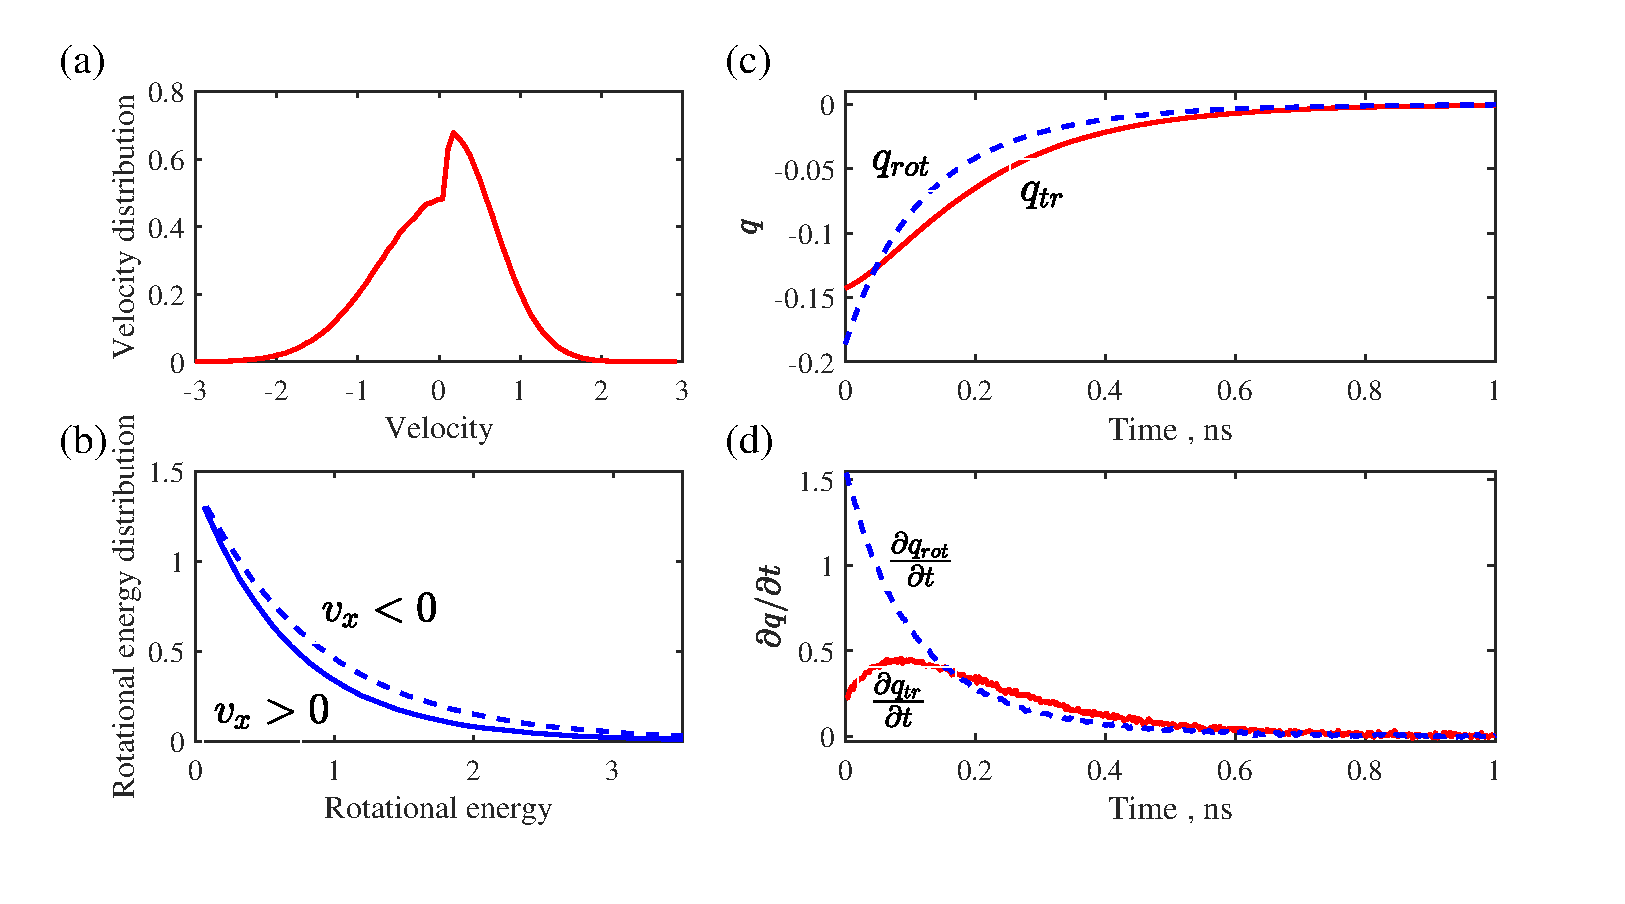
\includegraphics[scale=0.5,viewport=20 35 730 420,clip=true]{Fig/CalculateA.pdf}
	\caption{ (a) 初始状态用于激发平动热流的速度分布函数;横坐标由最概然速率 $v_m$ 归一化. (b) 初始状态用于转动热流的转动能分布函数; 横坐标由 $k_BT_0$归一化. (c, d) 氮气平动热流和转动热流的弛豫过程. 模拟参数为:公式\eqref{Z_DSMC}中的非弹性碰撞概率取$\Lambda=0.25$, 施密特数取$\text{Sc}=1/1.33$, 转动自由度取 $d_r=2$, 温度粘性指数取$\omega=0.74$. 图中数据来源于文献\cite{Li2021Uncertainty}.
	}
	\label{fig:CalculateA}
\end{figure}

图\ref{fig:CalculateA}(d)给出氮气的热流变化率的演化过程, 可以看出平动热流的时间导数随时间先增加后减小,这可以解释为平动热流与转动热流之间存在强耦合效应,即在平动热流衰减的同时得到了转动热流的补偿,且根据公式~\eqref{relax_flux} 可知,$A_{tr}$ 必定小于零. 



\begin{figure}[t]
	\centering
	\renewcommand{\figurename}{图}
	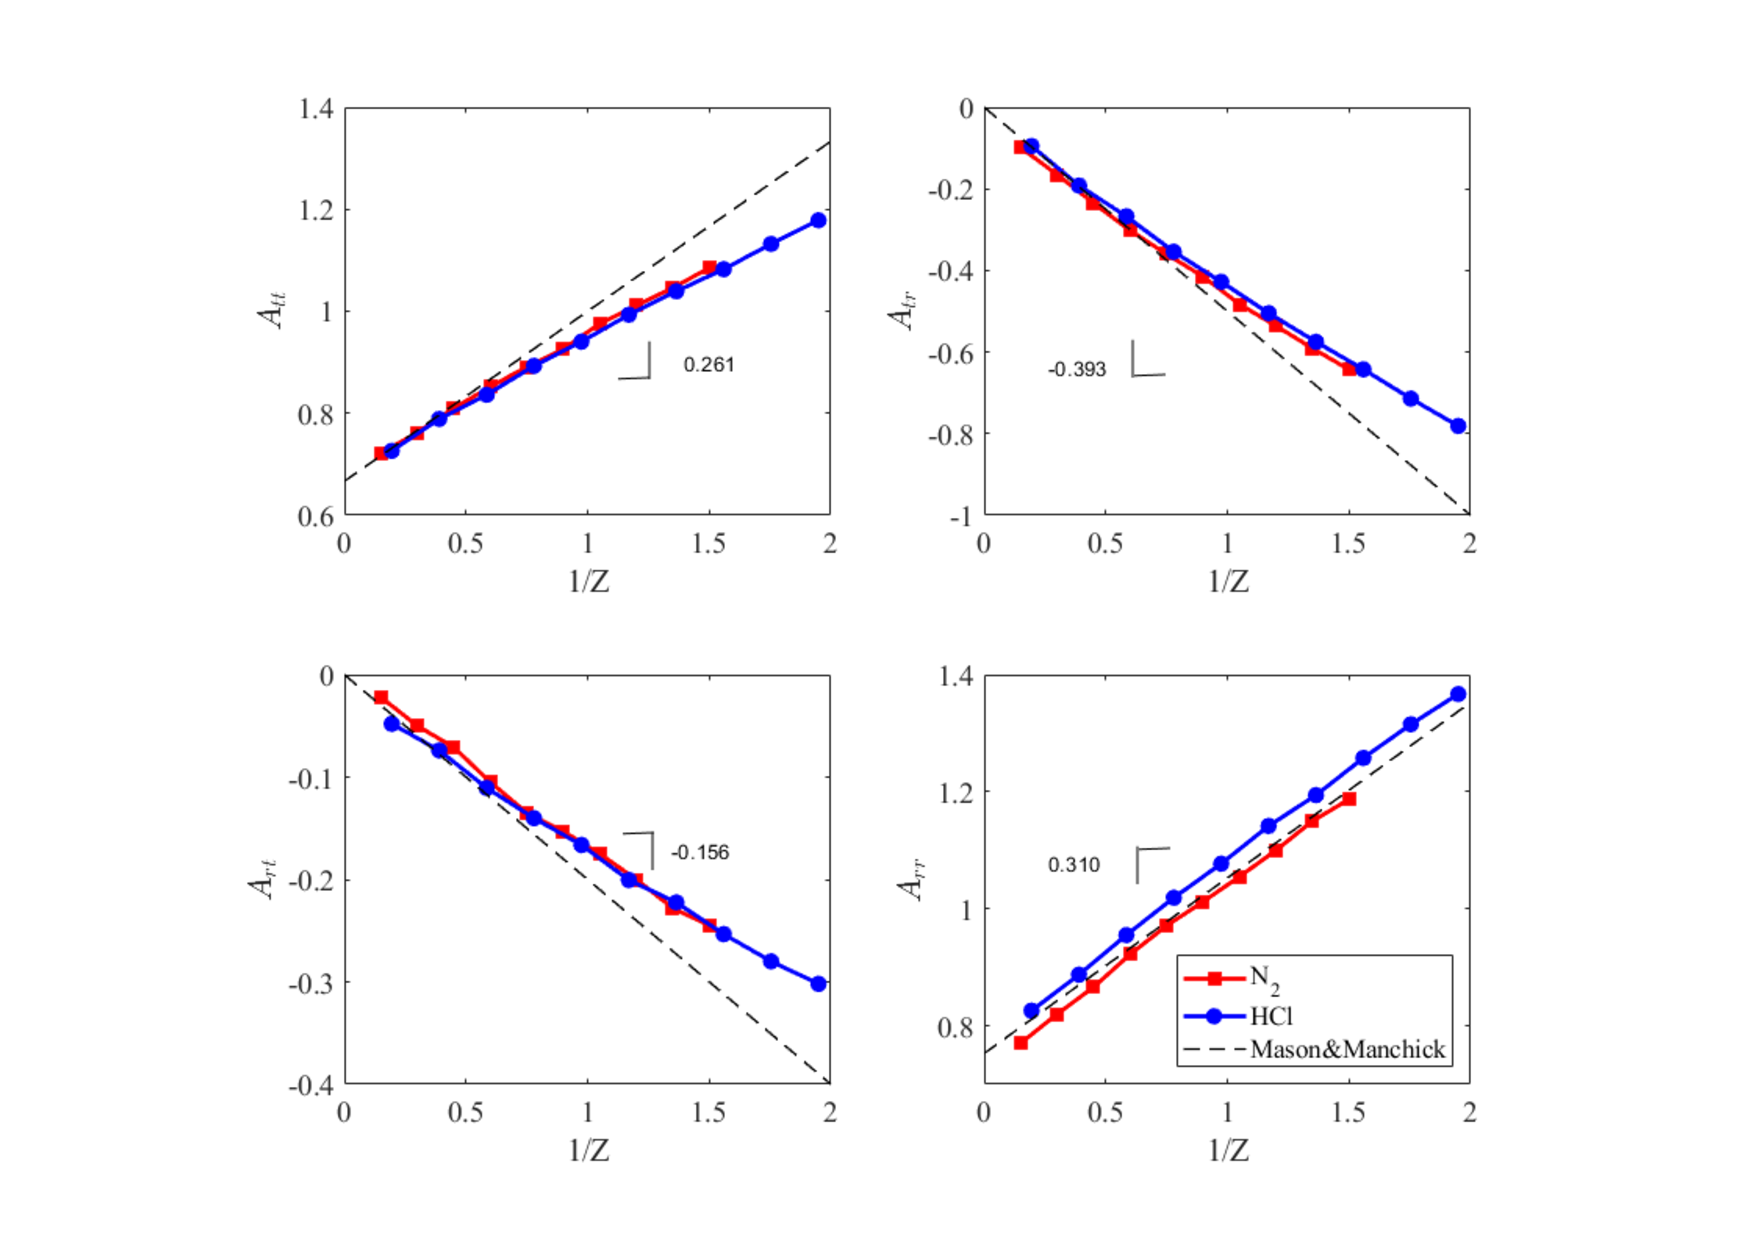
\includegraphics[scale=0.4,clip=true]{Fig/Matrix_A.pdf}
	\caption{
		根据理论公式\eqref{Mason_rates}从DSMC模拟中提取的热弛豫速率. 施密特数为$\text{Sc}=1/1.33$, 转动自由度为$d_r=2$; 对氮气和氯化氢,温度粘性指数$\omega$ 分别取0.74和1. 图中数据来源于文献\cite{Li2021Uncertainty}.\\
		The extracted rates $\bm{A}$ in the relaxation of heat fluxes from the DSMC simulation, as per Eq.~\eqref{Mason_rates}. The Schmidt number is $\text{Sc}=1/1.33$, and the rotational degree of freedom is $d_r=2$; the viscosity index for Nitrogen and hydrogen chloride is $\omega=0.74$ and 1, respectively. The figures are modified from figure 1 in reference \cite{Li2021Uncertainty}.
	}
	\label{fig:AZdsmc}
\end{figure}

图~\ref{fig:AZdsmc}显示通过最小二乘法求解线性回归问题~\eqref{relax_flux} 得到的热流弛豫速率 ${\mathbf{A}}$. 可以看出在相同的转动碰撞数$Z$和斯密特数下,氮气与氯化氢气体的热弛豫速率几乎相同. 另外,当 $Z\rightarrow\infty$ 时,有 $A_{tt}=2/3$, $A_{rr}=\text{Sc}$,$A_{tr}=A_{rt}=0$,可以得到与公式~\eqref{diffusion2}一致的结果. 图中虚线为Mason和Manchick的结果~\eqref{Mason_rates},由于忽略了$1/Z$的高阶项,其结果在$1/Z$较大时与DSMC的结果出现明显偏差.  %{\color{blue}这里需要指出的是,此处${\mathbf{A}}$的计算依赖于DSMC模拟中碰撞模型的选择,并不意味着在实际气体中一定具有相同的现象}. 


\begin{figure}[t]
	\centering
	\subfigure[氮气: $\frac{\rho{D'}}{\mu}=1.33$]{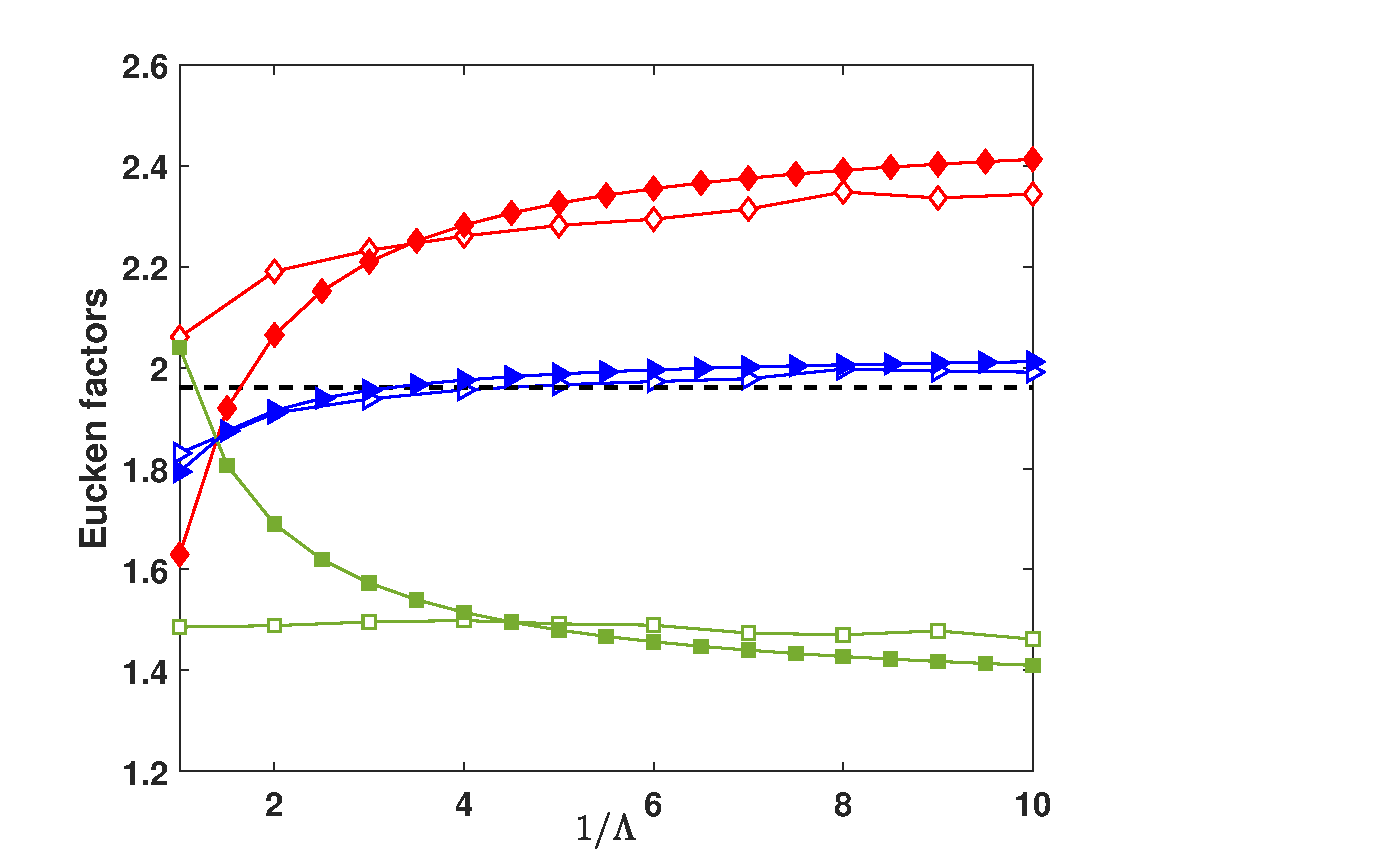
\includegraphics[scale=0.4]{Fig/Eucken_Nitrogen.pdf}}
	\subfigure[氯化氢: $\frac{\rho{D'}}{\mu}=0.89$]{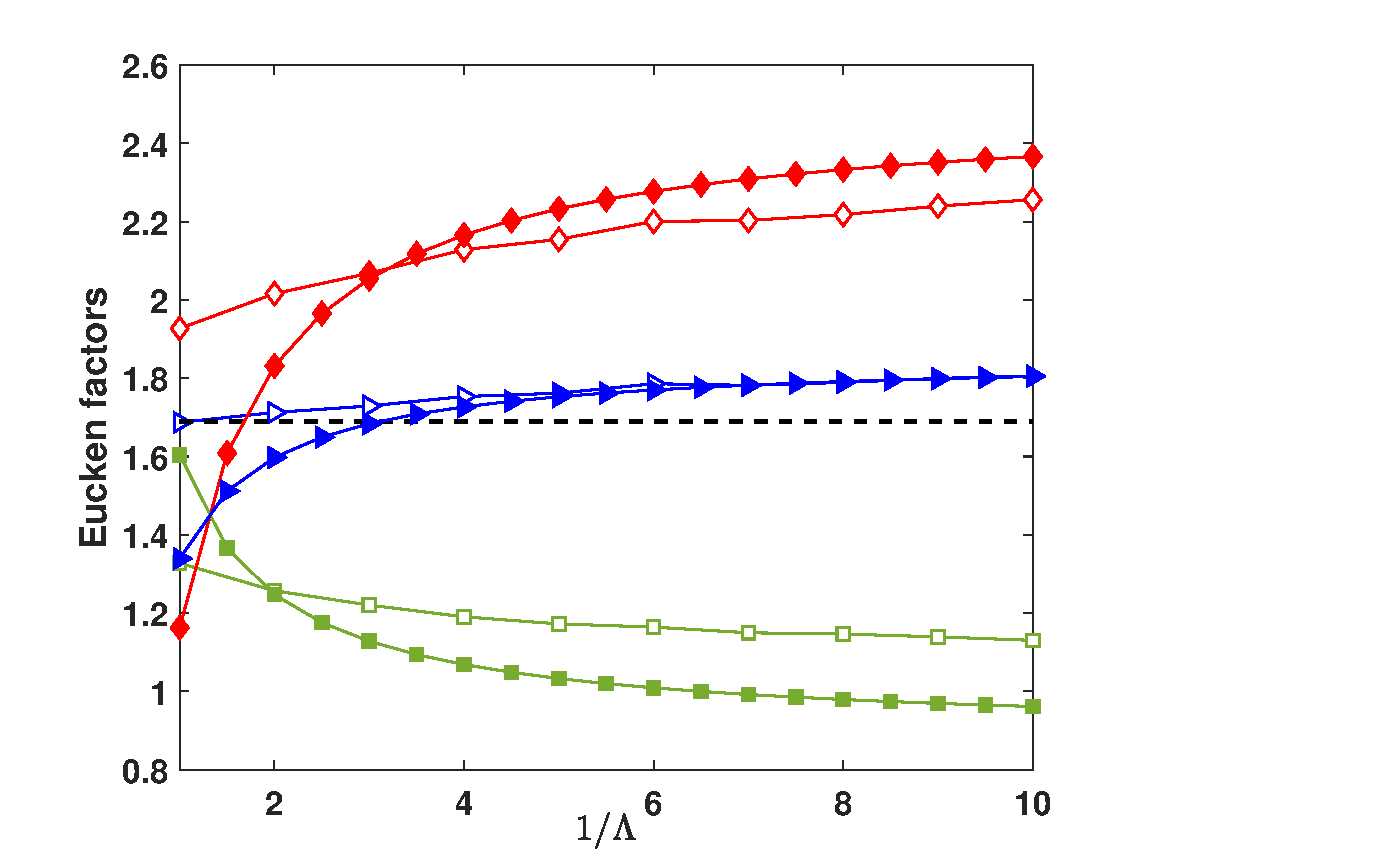
\includegraphics[scale=0.4]{Fig/Eucken_HCL.pdf}}
	\caption{ 
		室温下Eucken因子的解析解\eqref{Eucken}与DSMC数值解的对比. DSMC中使用可变软球模型,自扩散系数 $D$ 取值为 $D'$. 菱形、正方形、三角形分别表示平动、内能和总Eucken因子,实心点为解析解,空心点为DSMC结果,虚线表示 300~K 温度下实验测量的总Eucken因子. 图中数据来源于文献\cite{Wu2020JFM}\\
		The thermal conductivity obtained from the analytical solution~\eqref{Eucken} and the DSMC at room temperature, as a function of the inelastic collision probability $\Lambda$. The variable-soft-sphere model is used and the self-diffusion coefficient $D$ in DSMC takes the value of $D'$. Open diamonds, squares and triangles represent the translational, internal and total Eucken factors from Eq.~\eqref{Eucken}, respectively, while the filled symbols are the corresponding results from DSMC. Dashed lines show the total Eucken factor obtained from experiments at a temperature of 300~K. The figures are from reference \cite{Wu2020JFM}.
	}
	\label{fig:DSMC} 
\end{figure}

图~\ref{fig:DSMC}给出根据公式\eqref{trans_coeff}和\eqref{f_trf_rot}计算得到的Eucken因子,并与常温下的实验结果对比.  对于氮气,当施密特数取$1/1.33$时,通过选择特定的碰撞数$1/\Lambda\approx3.5$,DSMC可以恢复实验测量得到的总热导率,但由于缺少相应实验数据,我们无法分辨其是否能正确恢复平动与转动热导率分量. 若此温度下氮气的体积粘性要求 $1/\Lambda\not\approx3.5$,则DSMC给出的总热导率必然存在误差. 对于极性气体氯化氢,实验中常温下测得的总Eucken因子约为 $1.7$,但是从图~\ref{fig:DSMC}(a) 中,如果取施密特数为$1/1.33$,从DSMC中导出的总Eucken因子最小只能达到 $1.8$; 因此无论如何选择碰撞数,DSMC都不能恢复总热导率. 



从公式~\eqref{Eucken}可得,当气体种类确定时,转动碰撞数决定了体积粘性, 因此我们可以通过调整DSMC中的扩散系数  以恢复总热导率,见图~\ref{fig:DSMC}(b).  然而,即便在体积粘性与总热导率均与实验值相同的情况下,方程~\eqref{Eucken}的近似解与使用Larsen-Borgnakke模型的DSMC方法得到的平动热导率 $f_{tr}$ 并不一致,且两者的准确性都尚不确定. 对于氯化氢气体,极性分子的共振相互作用\cite{mason1962heat}导致 $\rho{}D'/\mu$ 从$ 1.33 $ 降低至 $ 0.89$,为了恢复实验测量的总热导率,从图~\ref{fig:DSMC}(b)可知,DSMC的非弹性碰撞概率约等于 $ 1 $,达到了平动能与内能交换的极限,因此并不是一个满足物理要求的值.  若选择合理的非弹性碰撞概率,则将要求DSMC中的有效扩散系数远小于自扩散系数. 这将带来另一个问题:对于多组分气体,扩散系数与热导率同等重要,而Larsen-Borgnakke模型难以同时正确恢复这两个输运系数,亟需改进. 




\section{分子气体的动理论模型及精度}\label{Kinetic_model_poly}



WCU方程的每一个内能能级都对应一个速度分布函数,因而计算代价巨大. 对于强激波问题,氮气的能级数可达到70,给数值求解带来了极大的困难\cite{Tcheremissine2008AIP}. 因此对WCU方程进行简化是非常必要的,而简化的基本原则与单原子气体相同,即需要满足必要的守恒律和平衡态分布,还需要尽量使各物理量的输运系数与WCU方程保持一致,例如,扩散系数、剪切粘性、体积粘性、热导率及其在各自由度下的分量等. 更接近本质的说法是,各输运系数对应的物理量的弛豫速率与实际气体保持一致. 学者们提出了许多描述分子气体稀薄效应的动理学模型方程,如Rykov模型和ES-BGK模型等. 如同在单原子气体中Gross-Jackson模型可以视为所有模型的源头,在分子气体中可以认为Hanson-Morse模型~\cite{Hanson1967PoF}是所有动理论模型的源头.

在小克努森数情况下,从简化模型方程和WCU方程推导出的纳维-斯托克斯方程必须是一致的. 事实上,这种一致性的根本要求是,模型方程中所对应的各个分子气体输运系数(例如:剪切粘性、体积粘性、热导率及其在各自由度下的分量等)需与原方程保持一致. 基于以上要求,

\subsection{Hanson-Morse线性化 模型} 

此模型在线性化情况下逼近WCU方程~\eqref{chapter1_WCU_Boltzmann0}的碰撞项. 这种构造方法类似于单原子气体的 Gross-Jackson模型\cite{GrossJackson1959},即通过对玻尔兹曼碰撞项进行正交多项式展开,并保证各多项式对应的宏观量的弛豫速率与WCU方程一致而获得. 对于分子气体,关于分子速度的多项式仍由麦克斯韦分子的本征函数\eqref{Wang_Chang}给出;关于内部能量的多项式的前两项取为1和$\epsilon=e_i-\bar{e}$,其中$\bar{e}$为平均内部能量\cite{WangCS}. 


分子气体的平衡态速度分布函数可表示为 $f_i=o_iF_{eq}$,其中
\begin{equation}
o_i=\frac{g_i\exp(-e_i/k_BT)}{\sum_j{}g_j\exp(-e_j/k_BT)}
\end{equation}
表征了内能为 $e_i$ 的分子比例. 在线性化问题中,通常考虑宏观速度为零的全局平衡态,并将速度分布函数写为如下形式:
\begin{equation}\label{polyatomic_lin_origin}
f_i(t,\bm{x},\bm{\xi})=o_if_{eq}(\bm{\xi})\left[1+\phi_i(t,\bm{x},\bm{\xi})\right],
\end{equation}
其中每个内部能级对应的扰动分布函数 $\phi_i$ 满足 $|\phi_i|\ll1$. 注意到为与上文的单原子线性化模型保持一致,这里的 速度 和 空间坐标分别通过最概然速率 $v_m$和特征尺寸 $\ell$ 进行无量纲化;时间通过$\ell/v_m$归一化,加速度通过 $v_m^2/\ell$无量纲化,内能$e_i$通过 $k_BT_0$ 无量纲化. 归一化后的扰动物理量可以通过对扰动分布函数求矩得到:
\begin{equation}
\begin{aligned}[b]
{n}_i=\int{f_{eq}}\phi_id\bm{\xi}, \quad
\bar{e} =\sum_io_ie_i,\\
[\bm{u},\sigma_{\alpha\beta}]=\sum_io_i\int{f_{eq}}\phi_i[\bm{\xi},\xi_{\langle \alpha}\xi_{\beta\rangle}]d\bm{\xi}, 
\quad\\
T_{t}=\sum_io_i\int{f_{eq}}\phi_i
\left(\frac{2}{3}\xi^2-1\right)d\bm{\xi}, \\
\bm{q}_{t}=\sum_io_i\int{f_{eq}}\phi_i
\left(\xi^2-\frac{5}{2}\right)\bm{\xi}d\bm{\xi}, \\
[T_{r},\bm{q}_{r}]=\sum_io_i\int{f_{eq}}\phi_i\epsilon_i
\left[\frac{2}{d_r},\bm{\xi}\right]d\bm{\xi}, 
\end{aligned}
\end{equation}
同时,总扰动密度为 ${n}=\sum_i{n}_io_i$.

若加速度为小量, WCU方程的线性化形式为
\begin{equation}\label{WCU_lin}
\frac{\partial \phi_i}{\partial{}t}
+{\bm{\xi}}\cdot\frac{\partial
	\phi_i}{\partial \bm{x}}
-2{\bm{a}}\cdot\bm{\xi}=\frac{\ell}{v_m}{J}_i,
\end{equation}
其中${J}_i$的形式与公式\eqref{Chapter1_Boltzmann_lin0}类似,不再赘述. 根据Hanson-Morse模型~\cite{Hanson1967PoF},
该线性化碰撞项可近似为\cite{Hanson1967PoF}
\begin{equation*}\label{HansonMorese_lin}
\begin{aligned}[b]
&{J}_i=-J_{030}(n_i+2\bm{\xi}\cdot\bm{u}-\phi_i)
+{2\sigma_{\alpha\beta}}(J_{020}-J_{030})
\xi_{\langle \alpha}\xi_{\beta\rangle}\\
&+T_{t}\left[ (-J_{030}+J_{100})\left(\xi^2-\frac{3}{2}\right)-\frac{3}{d_r}J_{100}{\epsilon} \right] \\
&+2\bm{\xi}\cdot\bm{q}_{t}\left[ (J_{110}-J_{030})\frac{2}{5}\left(\xi^2-\frac{5}{2}\right) -J_{011}^{110}\sqrt{\frac{4}{5d_r}}{\epsilon} \right]\\
&+T_{r}\left[ -J_{100}\left(\xi^2-\frac{3}{2}\right) +\left( \frac{3}{d_r}J_{100}-{J}_{030} \right){\epsilon} \right]\\
&+2\bm{\xi}\cdot\bm{q}_{r}\left[ -{J}_{011}^{110}\sqrt{\frac{4}{5d_r}}\left(\xi^2-\frac{5}{2}\right) +2(J_{011}-J_{030})\frac{{\epsilon}}{d_r} \right].
\end{aligned}
\end{equation*}
Hanson-Morse模型假设各内部能级的弛豫时间相同,则
与公式\eqref{Mason_rates}对应的弛豫率为
\begin{equation}\label{coefficient_Hason_Morse}
\begin{aligned}[b]
\tau=\frac{\mu}{p_t}, \\
J_{020}=-\tau^{-1}, \quad
J_{030}=-\frac{3}{2}\tau^{-1},\\
J_{100}=-\frac{1}{Z\tau}\frac{d_r}{3+d_r}, \quad
J_{110}=-\frac{2}{3\tau}-\frac{5}{6Z\tau}\frac{d_r}{3+d_r},\\
J_{011}^{110}=-\sqrt{\frac{5}{4d_r}}\frac{1}{Z\tau}\frac{d_r}{3+d_r}, \\
J_{011}=-\frac{\mu}{\rho{D'}}-\frac{3}{2(3+d_r)Z}.
\end{aligned}
\end{equation}


在自发瑞利-布里渊散射中,如果模型中包含应力偏量 $\sigma_{\alpha\beta}$,则该模型称为Tenti-S7模型~\cite{Boley1972CanJPhys,Tenti1974},其缺点在于不能得到实验散射光谱. Tenti-S6模型通过移除应力偏量 $\sigma_{\alpha\beta}$,即令模型中的$\sigma_{\alpha\beta}=0$,获得与实验一致的散射光谱. 实际上,如果不考虑内部能级,Tenti-S7和Tenti-S6模型分别退化为单原子ES-BGK模型和Shakhov模型,而在大多数情况下Shakhov模型的精度高于ES-BGK模型.

当在Hanson-Morse模型中移除应力偏量,为了复现应力偏量、能量弛豫、热流的弛豫过程,式~\eqref{coefficient_Hason_Morse}中的$J_{030}$应该改成$-1/\tau$. 同时,将系数 $J_{011}$ 修改为以下形式~\cite{Boley1972CanJPhys,Pan2004}:
\begin{equation}
J_{011}=-\frac{2d_r}{3(3+d_r)\tau}
\frac{\frac{1}{5}(3+d_r)+\frac{6+d_r}{4Z}+\frac{9}{16Z^2}f_u}
{\frac{2}{15}f_u\left(3+d_r\right)+\frac{d_r}{6Z}f_u-1},
\end{equation}
从而保证正确恢复热导率.
so that the thermal conductivity is exactly recovered.

Let's consider the Hanson-Morse model involving not the pressure tensor. 
\subsection{Hanson-Morse模型的约化及非线性化}\label{reduced_HM}
并定义 $\phi=\sum_io_i\phi_i$,
为了减小计算量,引入如下两个约化速度分布函数
\begin{equation}
\begin{aligned}[b]
&g=\sum_i{o_i}f_{eq}{\phi_i}, \\ 
&r=\sum_i{o_i}f_{eq}{\phi_i}(e_i-\bar{e}),
\end{aligned}
\end{equation}
消去内能自由度,则Hanson-Morse模型可以简化为
\begin{equation}
\begin{aligned}[b]
\frac{\partial g}{\partial{}t}
+{\bm{\xi}}\cdot\frac{\partial
	g}{\partial \bm{x}}
-2{\bm{a}}\cdot\bm{\xi}=\frac{\ell}{v_m}{J}_g,\\
\frac{\partial r}{\partial{}t}
+{\bm{\xi}}\cdot\frac{\partial
	r}{\partial \bm{x}}
-2{\bm{a}}\cdot\bm{\xi}=\frac{\ell}{v_m}{J}_r,
\end{aligned}
\end{equation}
其中
\begin{equation}\label{HansonMorse_JG}
\begin{aligned}[b]
&{J}_g=-J_{030}\left[ {n}+2\bm{\xi}\cdot\bm{u}+\bm{\xi}\cdot\bm{q}_{t} \frac{4}{15}\left(\xi^2-\frac{5}{2}\right)-g\right]\\
&-J_{030}T_{t}\left(\xi^2-\frac{3}{2}\right)+{2\sigma_{\alpha\beta}}(J_{020}-J_{030})
\xi_{\langle \alpha}\xi_{\beta\rangle} \\
&-(T_{r}-T_{t})J_{100}\left(\xi^2-\frac{3}{2}\right)\\
&-\bm{\xi}\cdot\left[\bm{q}_{t} \frac{2d_r}{3Z\tau(3+d_r)}
+2\bm{q}_{r} {J}_{011}^{110}\sqrt{\frac{4}{5d_{r}}} \right]\left(\xi^2-\frac{5}{2}\right),
\end{aligned}
\end{equation}
and
\begin{equation}\label{HansonMorse_JR}
\begin{aligned}[b]
{J}_r=& -{J}_{030}\left(\frac{d_r}{2}T_{r}+2\bm{\xi}\cdot\bm{q}_{r}-r\right)\\
&-\frac{3}{2}J_{100}(T_{t}-T_{r})\\
& 
-2\bm{\xi}\cdot\bm{q}_{t}J_{011}^{110}\sqrt{\frac{d_{r}}{5}} +2\bm{\xi}\cdot\bm{q}_{r} J_{011}.
\end{aligned}
\end{equation}
很明显,带下括号的项为能量与热流的弛豫项,因此,Hanson-Morse模型也可以改写为公式~\eqref{general_model}的通用形式.

至此,注意到单原子气体中Gross-Jackson模型与BGK、ES-BGK、Shakhov等模型的关系,我们可以通过类似于公式\eqref{nonlinearization}中展示的非线性化程序构造出分子气体的动理学模型. 即首先写出扰动量$g$ 和$r$对应的速度分布函数:
\begin{equation}
\begin{aligned}[b]
&G(t,\bm{x},\bm{v})=\sum_i{o_i}{f_i},\\
&R(t,\bm{x},\bm{v})=\sum_i{o_i}{f_i}e_i,
\end{aligned}
\end{equation}
并定义宏观量如下
\begin{equation}\label{macro_molecular}
\begin{aligned}[b]
&[n,\bm{u},T_t]=\int{}\left[1,\frac{\bm{v}}{n}, \frac{mc^2}{3nk_B}\right]Gd\bm{v},
\\
&[p_{ij},\bm{q}_{t}]=\int{}\left[mc_i{c_j},\frac{{mc^2}\bm{c}}{2}\right]Gd\bm{v},
\\
&[T_r,\bm{q}_{r}]=\int{}\left[\frac{2}{d_rnk_B},\bm{c}\right]R d\bm{v}.
\end{aligned}
\end{equation}
总热流定义为 $\bm{q}=\bm{q}_{t}+\bm{q}_{r}$,平动压力、转动压力和总压力分别定义为 $p_t=nkT_t, p_r=nkT_r$ and $p=nkT$.   注意此处$G$可以线性化为$G=f_{eq}(1+g)$, 而$R$应该线性化为$R=(d_rk_BT/2)f_{eq}(1+g+r)$.
其次,把速度分布函数的演化过程形式地写为
\begin{equation}\label{general_model}
\begin{aligned}[b]
\frac{\partial G}{\partial t}+\bm{v}\cdot \frac{\partial G}{\partial \bm{x}} +\bm{a}\cdot \frac{\partial G}{\partial \bm{v}}&
=\underbrace{\frac{G_t-G}{ \tau  }}_{\text{弹性}}+\underbrace{\frac{G_r-G_t}{ Z\tau}}_{\text{非弹性}},\\
\frac{\partial R}{\partial t}+\bm{v}\cdot \frac{\partial R}{\partial \bm{x}} +\bm{a}\cdot \frac{\partial R}{\partial \bm{v}}&
=\underbrace{\frac{R_t-R}{ \tau  }}_{\text{弹性}}+\underbrace{\frac{R_r-R_t}{ Z\tau}}_{\text{非弹性}}.
\end{aligned}
\end{equation}
最后,根据公式\eqref{HansonMorse_JG}和 \eqref{HansonMorse_JR}中的碰撞项,类比公式\eqref{nonlinearization},写出四个参考分布函数
$G_t$,$G_r$, $R_t$和 $R_r$的形式. 

例如,考虑Hanson-Morse模型中不出现应力偏量. 公式\eqref{HansonMorse_JG}中的第一行和第二行即为线性化Shakhov模型的碰撞项,可以非线性化为
\begin{equation}
\begin{aligned}[b]
&\frac{p_t}{\mu} \left\{ F_{eq}(T_t)\left[1+\frac{2m\bm{q}_{t} \cdot \bm{c}}{15k_BT_tp_t}\left(\frac{mc^2}{2k_BT_t}-\frac{5}{2}\right)\right]-G \right\}\\
&=\frac{p_t}{\mu} (G_t-G).
\end{aligned}
\end{equation}
结合非线性模型\eqref{general_model}中的非弹性碰撞项$(G_r-G_t)/Z\tau$, 可以选取
\begin{equation}
\begin{aligned}[b]
G_r&=F_{eq}(T)\left[1+\frac{2m\bm{q}' \cdot \bm{c}} {15k_BTp}\left(\frac{mc^2}{2k_BT}-\frac{5}{2}\right)\right],\\
\bm{q}'&=\left[1-\frac{5d_r}{2(3+d_r)}\right]\bm{q}_{t} +\frac{15}{2(3+d_r)}\bm{q}_{r},
\end{aligned}
\end{equation}
以在线性化情况下退化为公式\eqref{HansonMorse_JG}中的后两项,其中能量交换由$F_{eq}(T)$和$F_{eq}(T_t)$的差距而来,热流松弛由$\bm{q}'$决定.


\subsection{非线性模型}

然而,历史并没有选择这条非线性化路线, 而是由许多学者各自提出了非线性动理学模型~\cite{rykov1978macroscopic,holway1966new,andries2000gaussian, Gorji2011, wu2015kinetic,wang2017unified,Lizhihui2017,Titarev2018,Mathiaud2020}. 下面我们将先介绍主要的Rykov模型和ES-BGK模型,并揭示与Hanson-Morse模型的内在联系. 最后我们介绍吴模型.

\subsubsection{Rykov 模型}

原始的Rykov模型~\cite{rykov1978macroscopic}仅适用于无振动模态的双原子气体,但是构造思想可以直接拓展至多原子分子气体建模~\cite{wu2015kinetic}. 在该模型中,四个参考速度分布函数定义为:
\begin{equation}
\begin{aligned}[b]
G_t&=F_{eq}(T_t)\left[1+\frac{2m\bm{q}_{t} \cdot \bm{c}}{15k_BT_tp_t}\left(\frac{mc^2}{2k_BT_t}-\frac{5}{2}\right)\right],\\
G_r&=F_{eq}(T)\left[1+\omega_0\frac{2m\bm{q}_{t} \cdot \bm{c}} {15k_BTp}\left(\frac{mc^2}{2k_BT}-\frac{5}{2}\right)\right],\\
R_t&=\frac{d_rk_BT_r}{2}G_t+F_{eq}(T_t)(1-\text{Sc})\frac{m\bm{q}_{r} \cdot \bm{c}}{p_t},\\
R_r&=\frac{d_rk_BT}{2}G_r+F_{eq}(T)\omega_1(1-\text{Sc})\frac{m\bm{q}_{r} \cdot \bm{c}}{p}.
\end{aligned}
\end{equation}

选取弹性碰撞弛豫时间$\tau={\mu}/{p_t}$以及适当的转动碰撞数$Z$, 可保证恢复正确的剪切粘性和体积粘性.
四个热流弛豫系数为
\begin{equation}
\begin{aligned}[b]
&A_{tt}=\frac{2}{3}\left(1+\frac{1-\omega_0}{2Z}\right),\\ &A_{rr}=\text{Sc}+\frac{(1-\text{Sc})(1-\omega_1)}{Z},\\
&A_{tr}=A_{rt}=0.
\end{aligned}
\end{equation}
因此通过公式~\eqref{f_trf_rot}可以得到Eucken因子的表达式如下:
\begin{equation}\label{Rykov_f}
\begin{aligned}[b]
f_{tr}&=\frac{5}{2}\left(1+\frac{1-\omega_0}{2Z}\right)^{-1},\\
f_{rot}&=\left(\text{Sc}+\frac{(1-\text{Sc})(1-\omega_1)}{Z}\right)^{-1}.
\end{aligned}
\end{equation}
这说明,在Rykov模型中,可通过调整自由参数 $ \omega_0 $ 和 $ \omega_1 $ 修改Eucken系数.

当$Z\rightarrow\infty$,该模型退化为单原子气体的Shakhov模型. 如果将其线性化,可以得到类似于\ref{reduced_HM}中的约化Hanson-Morse模型. 不同之处在于空间均匀系统中,Rykov模型中平动和转动热流的弛豫不会相互干扰,这是因为公式\eqref{trans_coeff}中$A_{tr}=A_{rt}=0$.


\subsubsection{ES-BGK 模型}

Holway通过最大熵原理提出了ES-BGK模型,该模型保留了标准BGK模型的数学简便性,并且能够恢复正确的普朗特数,同时满足熵增定理~\cite{holway1966new,andries2000gaussian}. 速度分布函数的演化方程为:
\begin{equation}
\begin{aligned}[b]
\frac{\partial G}{\partial t}+\bm{v}\cdot \frac{\partial G}{\partial x} +\bm{a}\cdot \frac{\partial G}{\partial \bm{v}}&=\frac{1}{ \tau  }\left(f_r^{ES}-G\right),\\
\frac{\partial R}{\partial t}+\bm{v}\cdot \frac{\partial R}{\partial x}+\bm{a}\cdot \frac{\partial R}{\partial \bm{v}}&=\frac{1}{ \tau }\left(\frac{d_r}{2}k_BT_{rel}f_r^{ES}-R\right),
\end{aligned}
\end{equation}
其中,弛豫温度 $T_{rel}$ 定义为转动温度与总温度的加权平均值 
\begin{equation}
T_{rel}=\left(1-\frac{1}{Z}\right){T_r}+\frac{T}{Z},
\end{equation}
参考分布函数$f_r^{ES}$由公式\eqref{ellipsoidal_model}给出,但是此处
\begin{equation}\label{Gaussian}
\begin{aligned}[b]
\lambda_{ij}=\left(1-\frac{1}{Z}\right)
\left[(1-b)\frac{k_BT_t}{m}\delta_{ij}+b\frac{p_{ij}}{nm}\right]
+\frac{k_BT}{Zm}\delta_{ij}.
\end{aligned}
\end{equation}
当$Z\rightarrow\infty$,转动和平动能量交换消失,因此模型方程退化为单原子气体的ES-BGK方程.

	with $\bm{I} $ being the unit tensor and $ \nu $ the other adjustable parameter in the range of $ -1/2\leq \nu \le 1 $. In~\eqref{Gaussian}, $B^{-1}$ and $\det(B)$ are the inverse and determinant of $B$, respectively.
取弹性碰撞弛豫时间$\tau=\mu/p_t\Pr$及适当的转动碰撞数$Z$, 则分子气体的剪切和体积粘性自动满足要求. 
其中普朗特数可以通过调整$b$的取值得到:
\begin{equation}\label{Pr}
\Pr=\frac{1}{1-b+b/Z}.
\end{equation}
为使参考分布函数有界且在物理上有意义,要求$ -1/2\leq {b} \le 1 $ 和 $ Z\ge 1 $. 因此,普朗特数范围为 $ 2/3 \leq \Pr \le +\infty$. 对于大部分双原子分子来说,普朗特数大约为$5/7$, 因此可以保证要求. 

与Rykov模型一样,ES-BGK模型的平动热流和转动热流的弛豫过程互不干涉;从它们的弛豫率可知,
Eucken因子可以表达为
\begin{equation}\label{eq:ES_ftr_frot}
\begin{aligned}[b]
&f_{tr}=\frac{5}{3\Pr},\\
&f_{rot}=\frac{1}{\Pr}=\frac{3+d_r}{5+d_r}f_{eu}.
\end{aligned}
\end{equation}
注意到,对于多原子ES-BGK模型,平动Eucken因子与转动Eucken因子的比值始终为$ 5/3 $,并且Eucken因子完全由普朗特数决定. 



\subsubsection{吴模型}

上述气体动理学模型的弛豫时间 $ \tau $ 都与分子速度无关,与玻尔兹曼方程的弛豫时间不相符. 因此,在正激波问题中,Rykov模型计算得到的结果可能会出现波前温升的误差,且随着马赫数的增加,这一偏离显著增长. 由此,为了提高模型方程准确性,吴雷等人首先将Rykov模型中的弹性碰撞项 $ ({G_t}-G)/\tau $ 替换为单原子玻尔兹曼方程的碰撞项 $ Q(G) $,以使弹性碰撞弛豫时间是分子速度的函数~\cite{wu2015kinetic};其后,又考虑引入更为准确的热流弛豫过程~\cite{Li2021Uncertainty},从而在相同参数条件下,得到更为符合DSMC的模拟结果. 

吴模型的演化方程为:
\begin{equation}\label{Wu_model}
\begin{aligned}[b]
\frac{\partial G}{\partial t}+\bm{v}\cdot \frac{\partial G}{\partial x}+\bm{a}\cdot \frac{\partial G}{\partial \bm{v}}&=Q(G)+\frac{G_r-G_t}{ Z\tau  },\\
\frac{\partial R}{\partial t}+\bm{v}\cdot \frac{\partial R}{\partial x} +\bm{a}\cdot \frac{\partial R}{\partial \bm{v}}&=\frac{R_t'-R}{ \tau  }+\frac{R_r-R_t}{ Z\tau  }.
\end{aligned}
\end{equation}
式中,$ R_t'=(d_r/2)k_BT_r(\tau Q+G) $, 弛豫时间为 $\tau=\mu/p_t$,对应的参考速度分布函数为:
\begin{equation}
\begin{aligned}[b]
G_t&=F_{eq}(T_t)\left[1+\frac{2m{\bm{q}_{t}} \cdot \bm{c}}{15k_BT_tp_t}\left(\frac{mc^2}{2k_BT_t}-\frac{5}{2}\right)\right],\\
G_r&=F_{eq}(T)\left[1+\frac{2m\bm{q}' \cdot \bm{c}} {15k_BTp}\left(\frac{mc^2}{2k_BT}-\frac{5}{2}\right)\right],\\
R_t&=\frac{d_rk_BT_r}{2}G_t, \\
R_r&=\frac{d_rk_BT}{2}G_r+F_{eq}(T)\frac{m\bm{q}'' \cdot \bm{c}}{p}.
\end{aligned}
\end{equation}

为了恢复热流弛豫过程~\eqref{relax_flux},选取 ${\bm{q}'}$ 和 ${\bm{q}''}$ 如下:
\begin{equation}
\begin{aligned}[b]
\bm{q}'&=\left[-3Z( A_{tt}-\frac{2}{3})+1\right]\bm{q}_{t}-3ZA_{tr}\bm{q}_{r},\\
\bm{q}''&=-Z\left[A_{rt} q_t+(A_{rr}-1)\bm{q}_{r}\right].
\end{aligned}
\end{equation}


当$Z\rightarrow\infty$,吴模型完全退化为单原子玻尔兹曼方程. 另一方面,如果将玻尔兹曼碰撞项换回Shakhov碰撞模型,在线性化的情况下,吴模型则完全与\ref{reduced_HM}中的约化Hanson-Morse模型一致.


Eucken因子同样可以通过公式~\eqref{f_trf_rot}计算,此模型提供了两个调整Eucken因子的自由度,因此能够保证恢复全部输运系数.


\subsection{模型方程精度比较}\label{sec:results}




\begin{figure*}[t]
	\centering
	{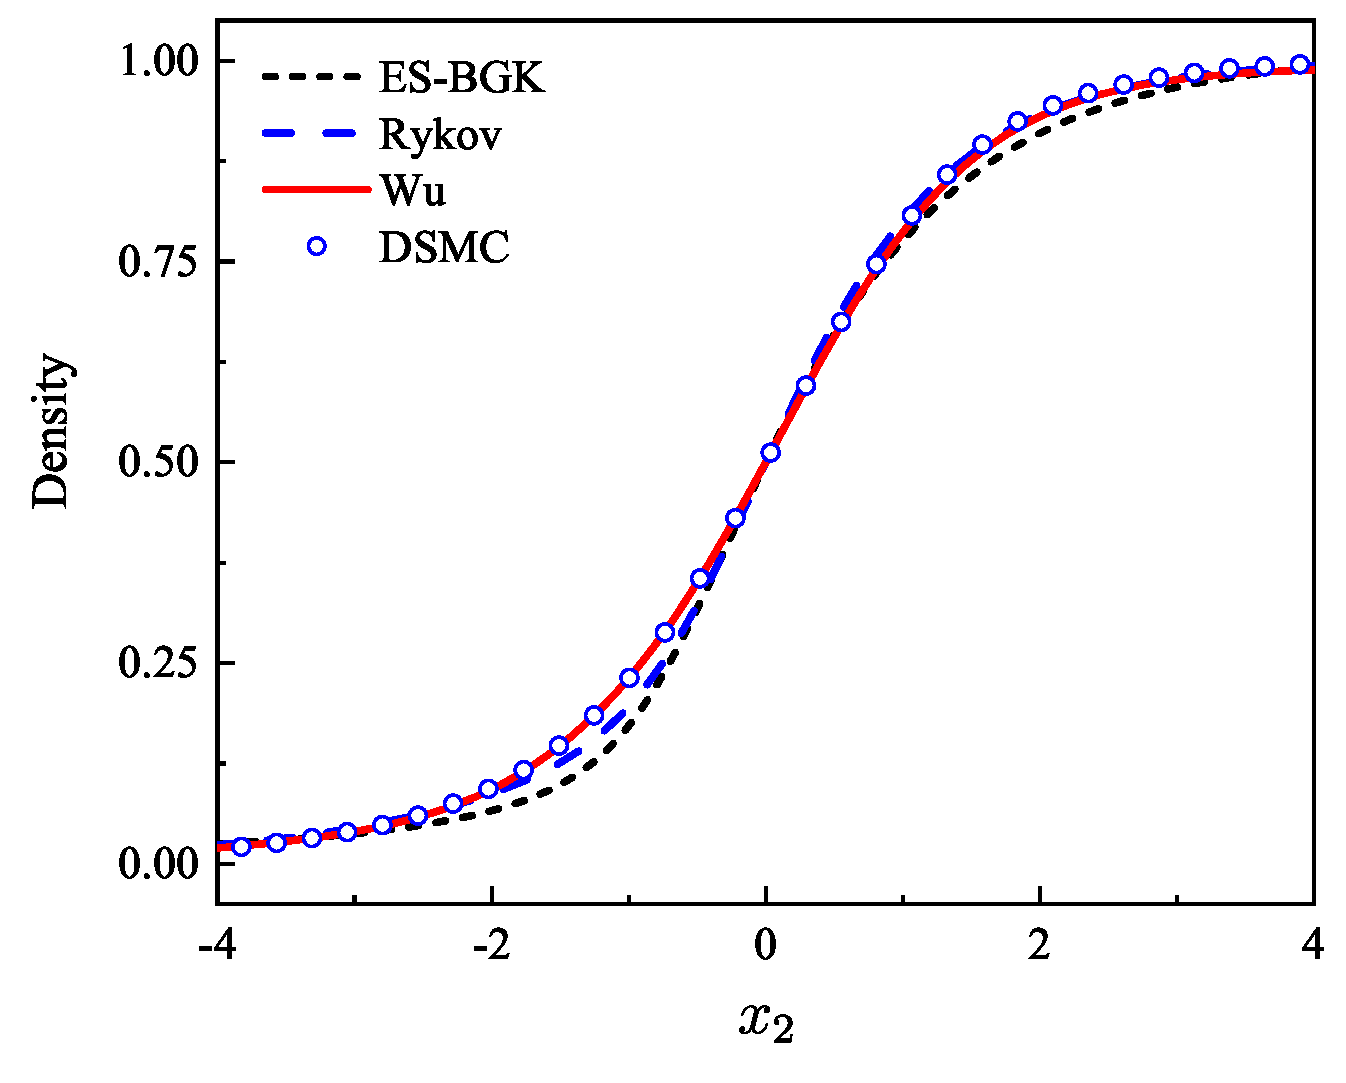
\includegraphics[scale=0.3,clip=true]{Fig/01NSW1.eps}} \quad
	{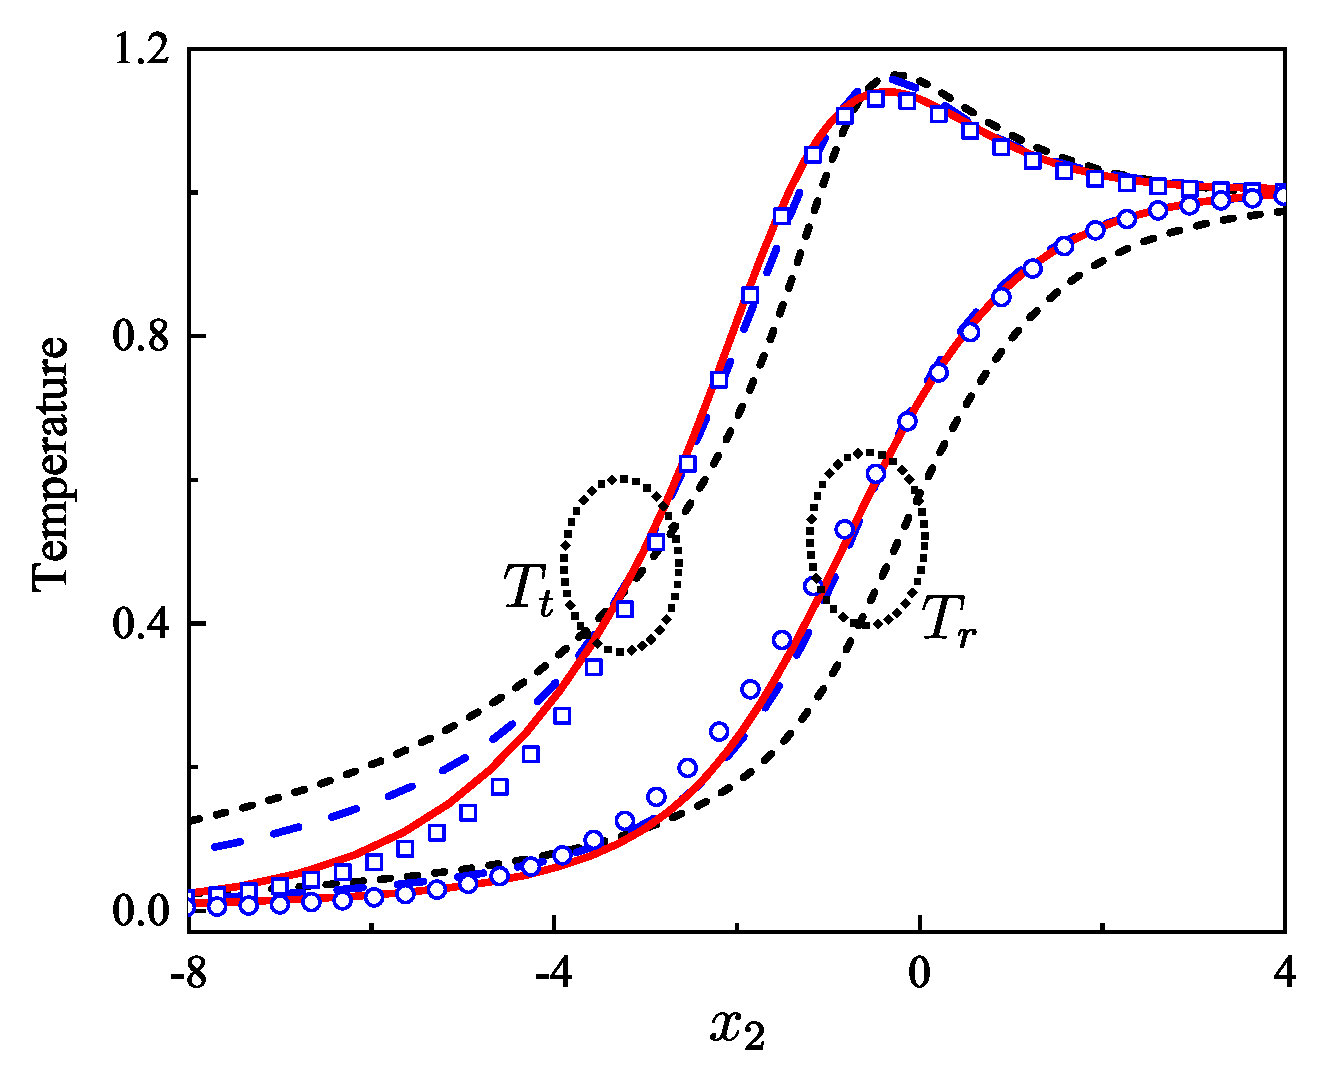
\includegraphics[scale=0.3,clip=true]{Fig/01NSW2.eps}} \\
	\vskip 0.5cm
	{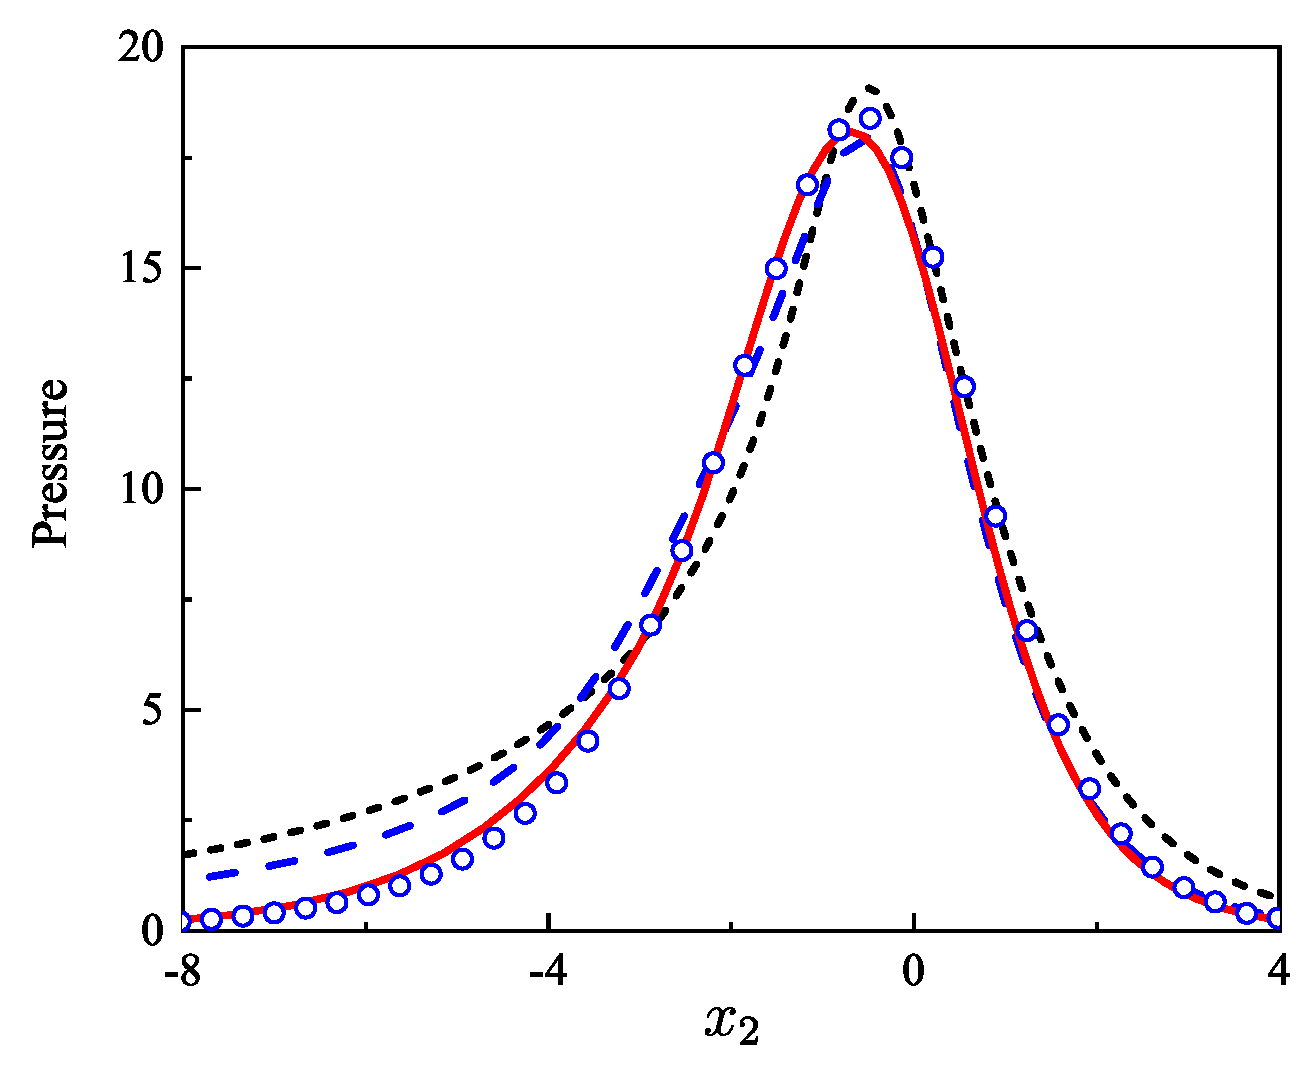
\includegraphics[scale=0.3,clip=true]{Fig/01NSW3.eps}} \quad
	{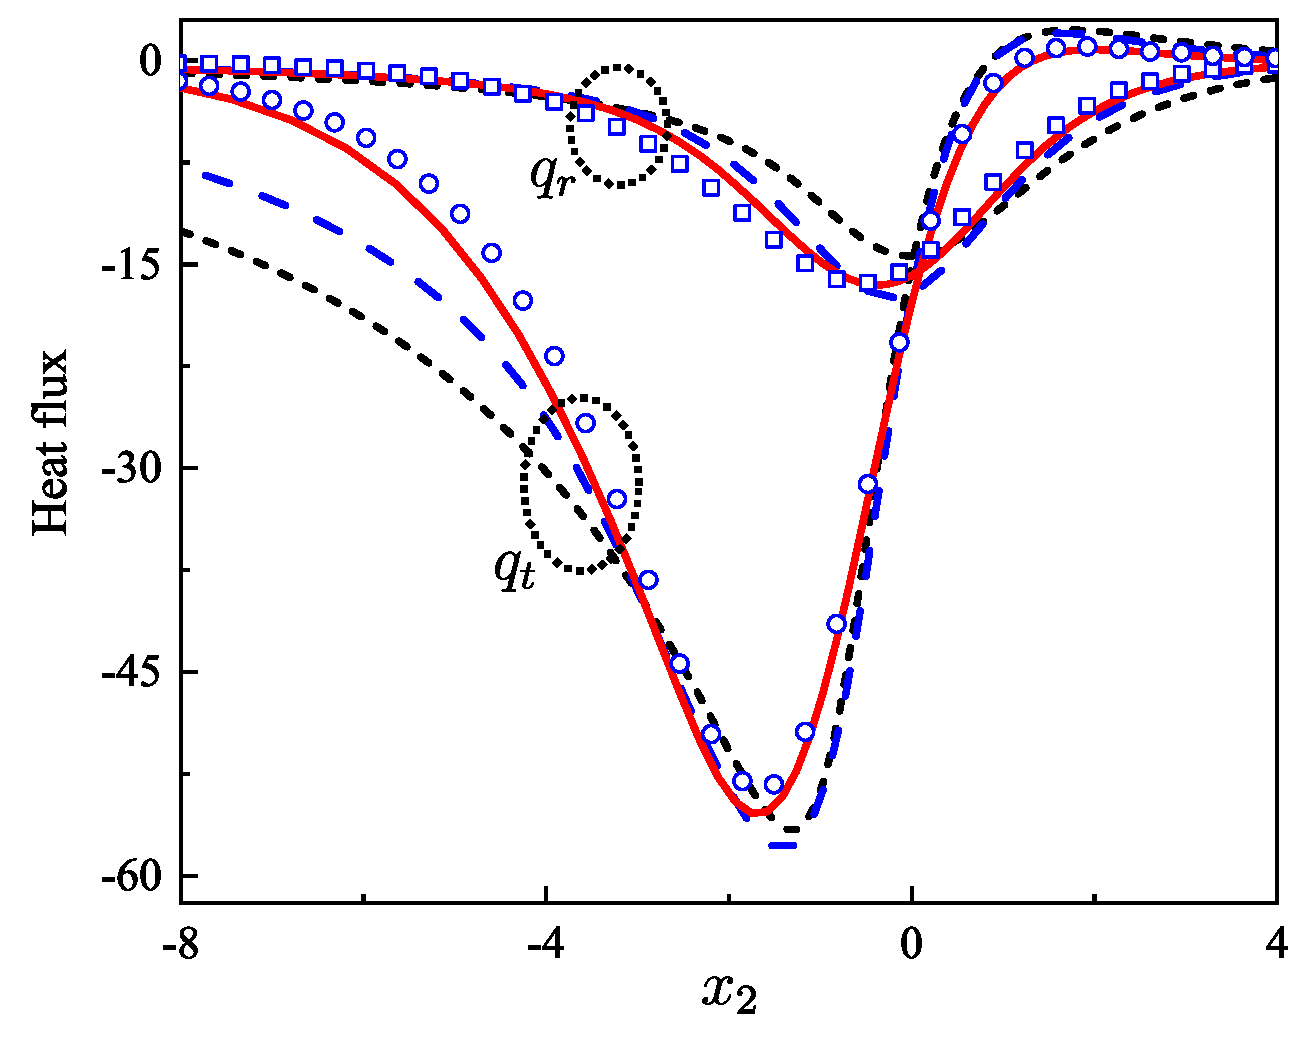
\includegraphics[scale=0.3,clip=true]{Fig/01NSW4.eps}}
	\caption{ 不同动理学模型预测的马赫数为7的氮气正激波的密度、温度,应力偏量$\sigma_{22}$和热流的对比. \\
		Comparisons in the density, temperature, stress, and heat flux between different kinetic models for a normal shock in Nitrogen gas with Mach number 7. 
	}
	\label{fig:nsw_n2_Ma7}
\end{figure*}




\begin{table}[t]
	\centering
	\caption{不同动理学模型和DSMC模拟中所使用的Eucken因子与热弛豫速率. 氮气的Eucken因子为$f_{eu}=1.993$. \\
		Eucken factors and heat flux relaxation rates used in different gas kinetic models and DSMC. The total Eucken factor of the Nitrogen at room temperature is $f_{eu}=1.993$. }
	\begin{tabular}{ccccc}
		\specialrule{0.0em}{2pt}{2pt}
		\hline \hline
		\specialrule{0.0em}{2pt}{2pt}
		& ES-BGK & Rykov & Wu & DSMC \\
		\specialrule{0.0em}{2pt}{2pt}
		\hline
		\specialrule{0em}{2pt}{1pt}
		$f_{tr}$    & 2.373   & 2.365 & 2.365 & 2.365  \\ \specialrule{0em}{2pt}{1pt}
		$f_{rot}$   & 1.424   & 1.436 & 1.436 & 1.436  \\ \specialrule{0em}{2pt}{1pt}
		$A_{tt}$    & 0.702   & 0.705 & 0.786 &  0.786   \\ \specialrule{0em}{2pt}{1pt}
		$A_{tr}$    &  0      &   0   & -0.201 &   -0.201  \\ \specialrule{0em}{2pt}{1pt}
		$A_{rt}$    &  0      &   0   & -0.059 &  -0.059 \\ \specialrule{0em}{2pt}{1pt}
		$A_{rr}$    & 0.702   & 0.696 & 0.842 &  0.842 \\ \specialrule{0em}{2pt}{1pt}
		\hline \hline
		\label{Eucken_Calculate}
	\end{tabular}
\end{table}


以下,以正激波结构,库特流、热蠕动、以及二维热驱动问题为例,比较不同模型描述稀薄气体流动的精度. 模拟中,分子气体为氮气,转动自由度 $ d_r=2$,模型中的相关参数选为 $Z=2.6671,\omega=0.74$, 施密特数$\text{Sc}=1/1.33$. 吴模型中的热弛豫系数矩阵$\bm{A}$来自\ref{thermal_exp_DSMC}中的DSMC模拟,从而保证吴模型的Eucken因子为$f_{eu}=1.993$, $f_{tr}=2.365$, 和$f_{rot}=1.436$,与DSMC保持一致;此外,我们进一步假设这些参数不随温度变化. Rykov模型可以通过公式~\eqref{Rykov_f} 调整$\omega_0$ 和 $\omega_1$ 恢复正确的Eucken系数. 从公式~\eqref{eq:ES_ftr_frot} 可知,ES-BGK模型只有一个自由度来恢复总Eucken系数,即ES-BGK模型没有分辨平动Eucken系数和转动Eucken系数的机制. 幸运的是,对于氮气,ES-BGK模型给出的平动和转动热导率与DSMC非常接近,见表~\ref{Eucken_Calculate}中关于Eucken参数的汇总. 再次强调,ES-BGK和Rykov模型中平动和转动热流的弛豫过程是相互独立的.


引入参考密度 $n_0$、参考温度 $T_0$、最概然速率 $v_m=\sqrt{2k_BT_0/m}$、参考压力 $n_0k_BT_0$、参考热流 $n_0k_BT_0v_m$. 宏观量通过参考值进行无量纲化,且无量纲克努森数定义为:
\begin{equation}
\text{Kn}=\frac{\mu(T_0)}{n_0\ell}\sqrt{\frac{\pi}{2mk_BT_0}},
\end{equation}
用于表征流动的稀薄程度, 其中$\ell$ 为流动特征长度. 

在以下各研究问题中,气体在固体表面的反射均用完全漫反射作为边界条件,即气体反射速度分布为满足固体表面宏观量的麦克斯韦分布。在数值解法上,使用离散速度法求解动理学模型,快速谱方法求解玻尔兹曼碰撞项\cite{Wu2017Physica},开源软件SPARTA进行DSMC模拟. 




\begin{figure*}[t]
	\centering
	{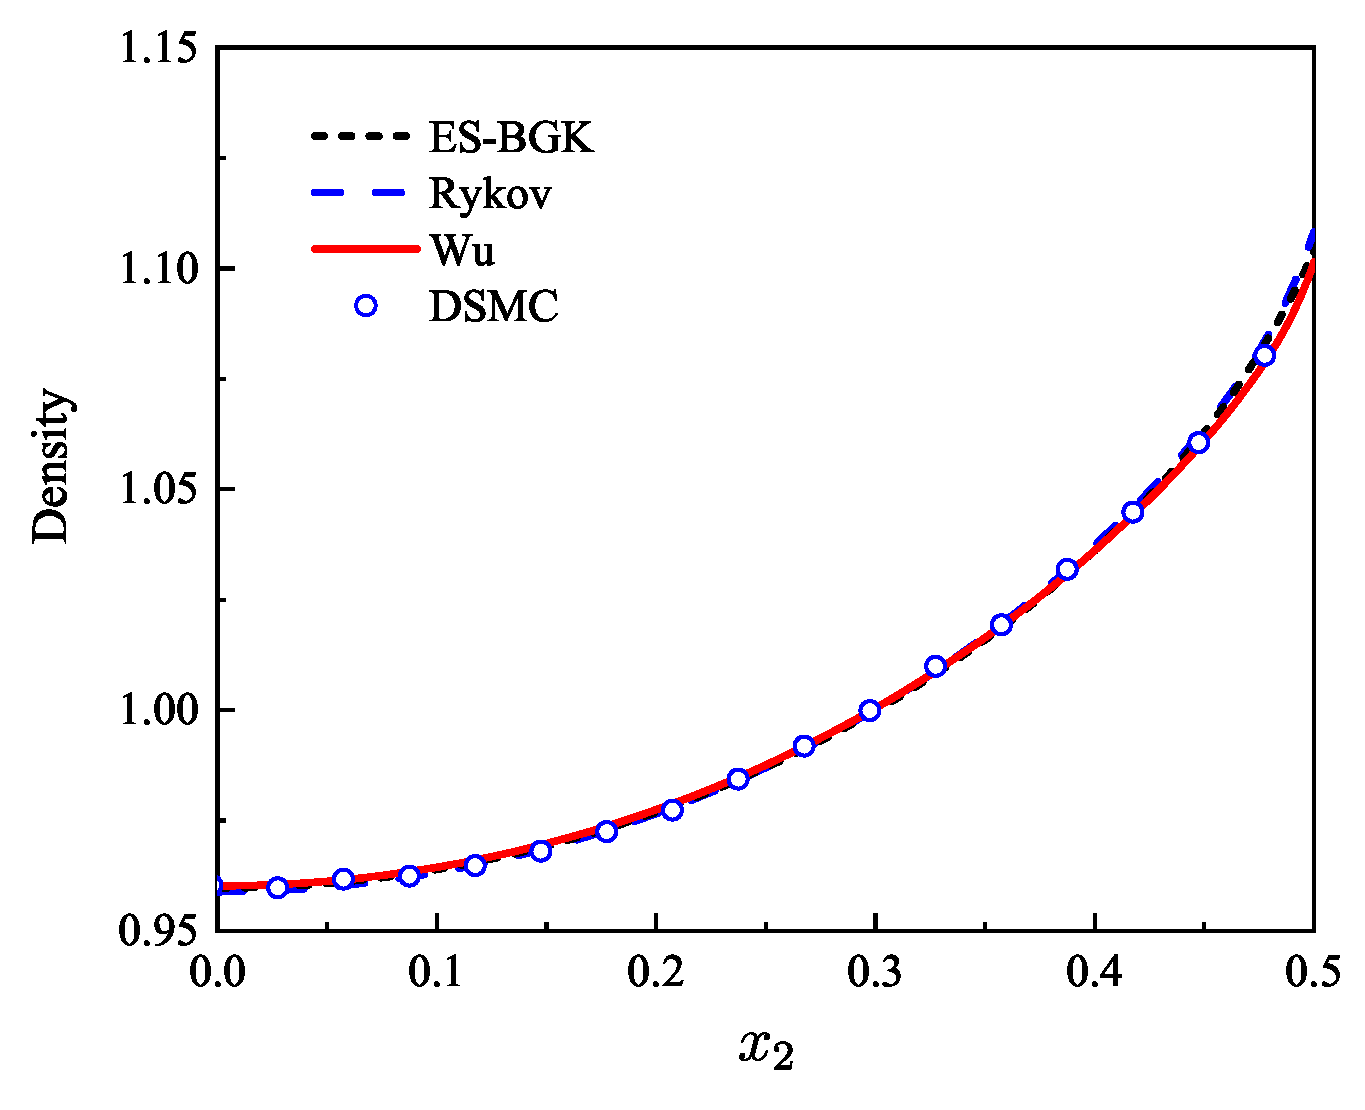
\includegraphics[scale=0.25,clip=true]{Fig/04CF1.eps}} \quad
	{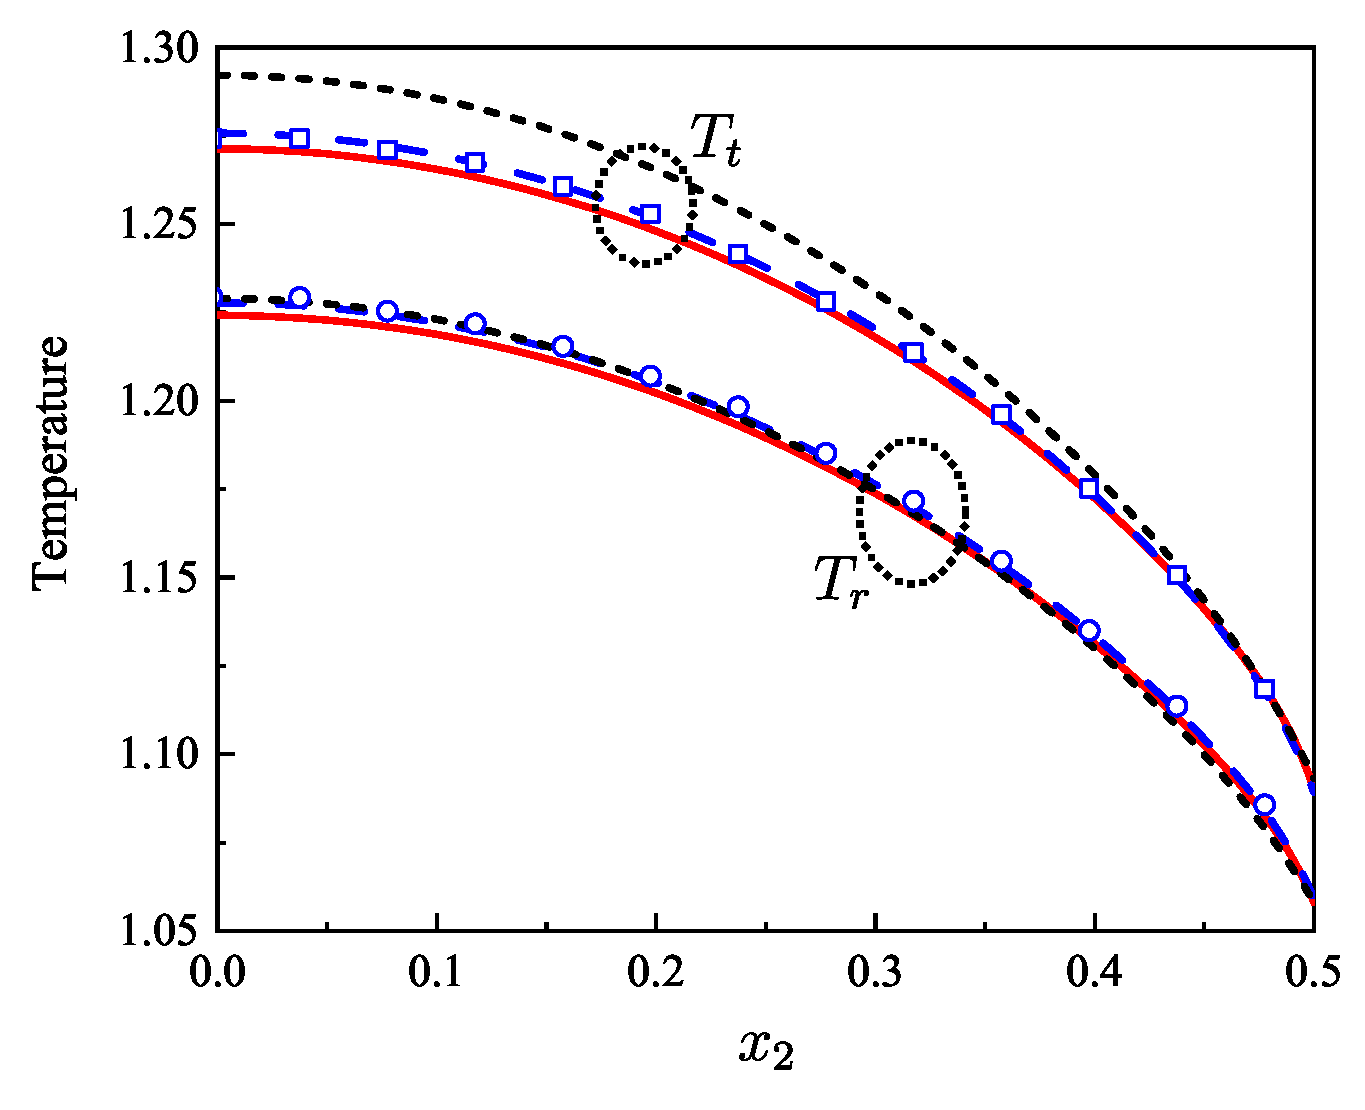
\includegraphics[scale=0.25,clip=true]{Fig/04CF2.eps}}\quad
	{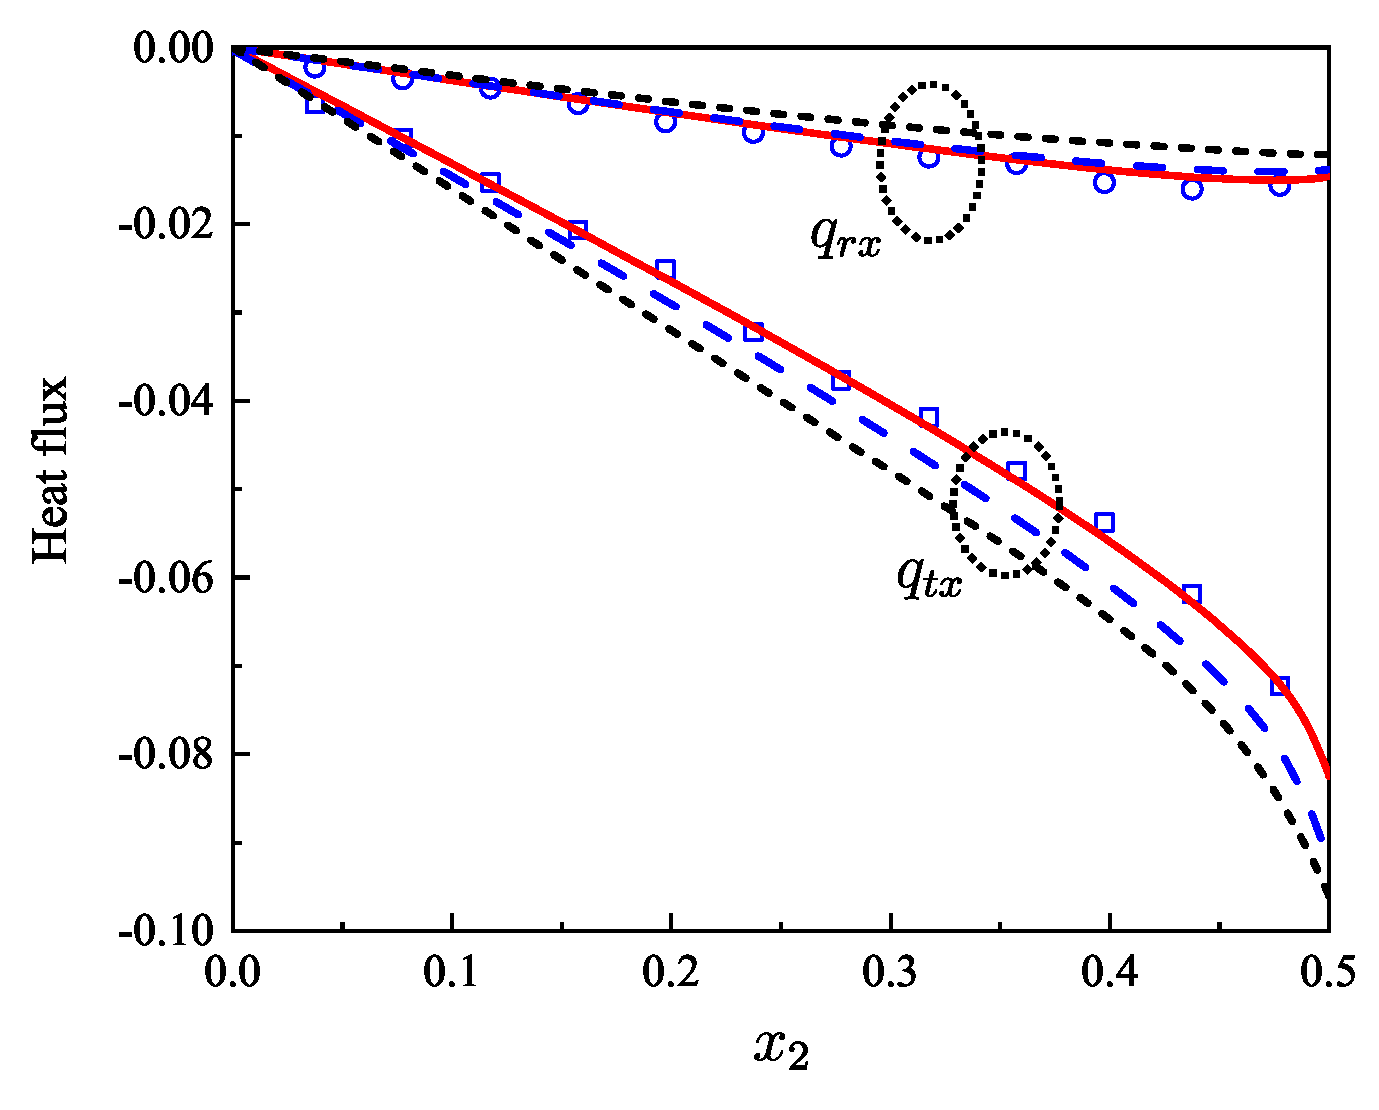
\includegraphics[scale=0.25,clip=true]{Fig/04CF3.eps}} \\
	\vskip 0.5cm
	{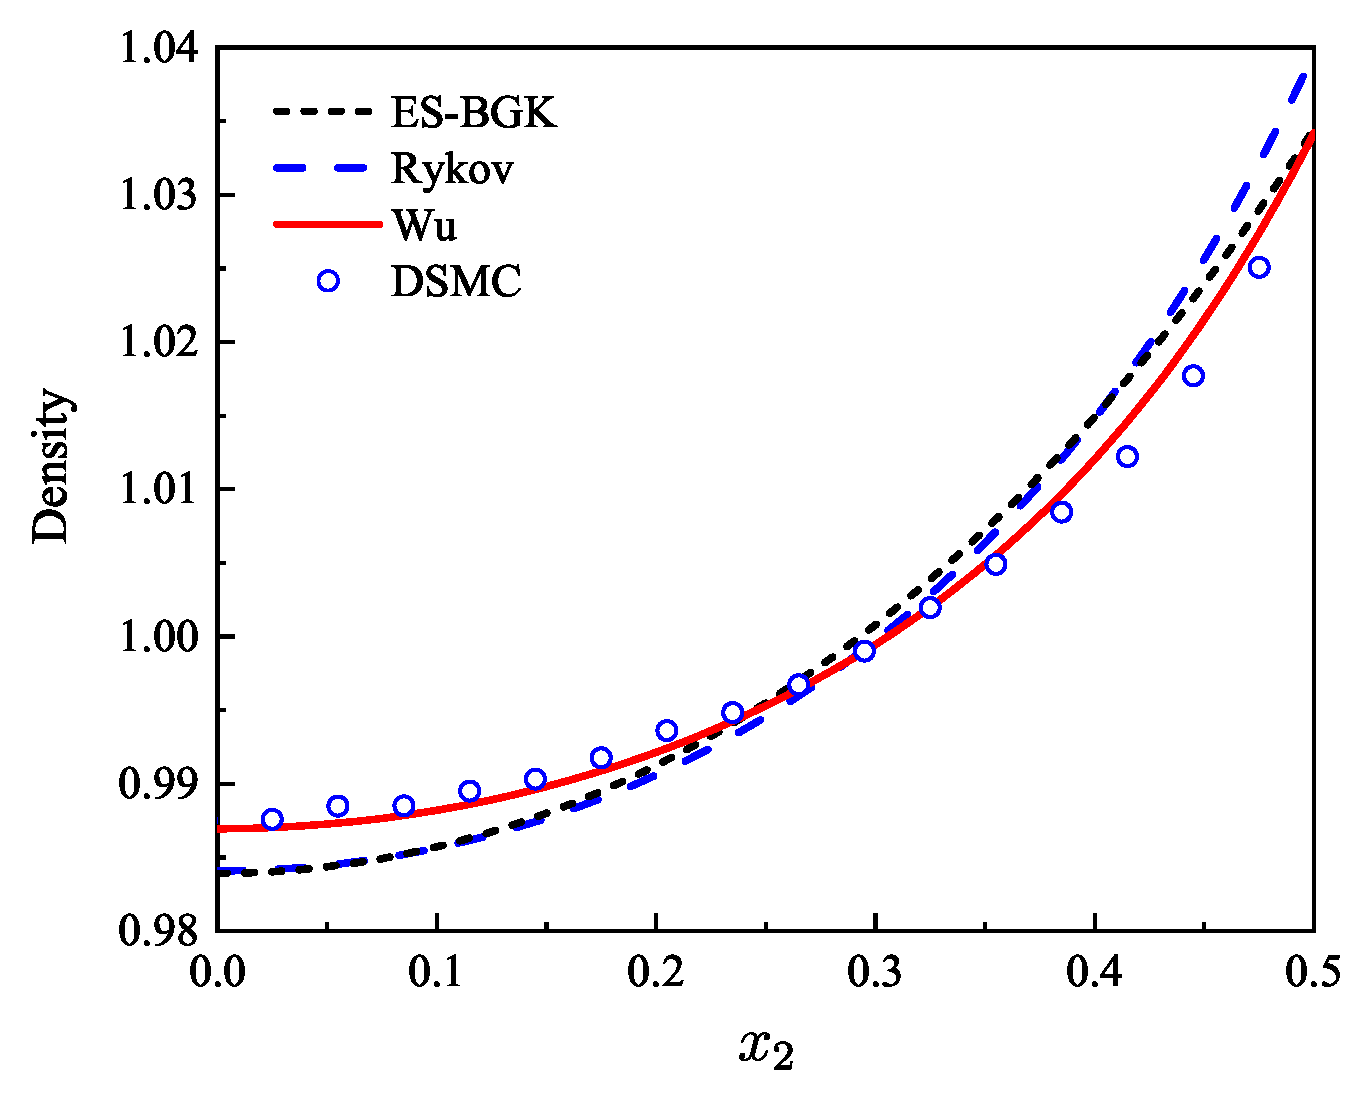
\includegraphics[scale=0.25,clip=true]{Fig/04CF4.eps}}\quad
	{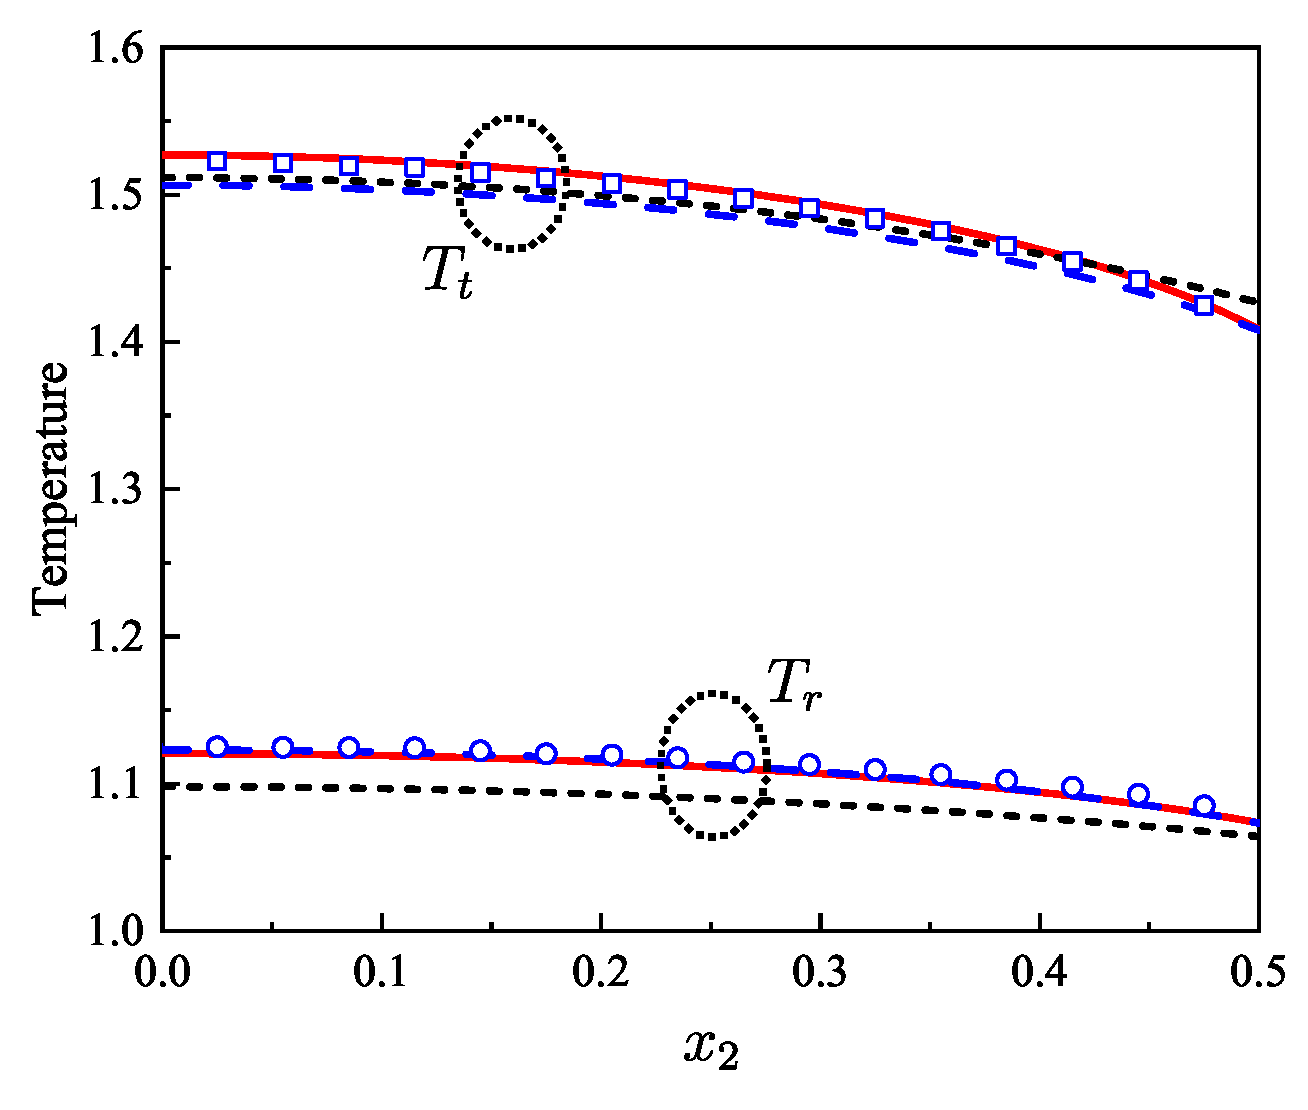
\includegraphics[scale=0.25,clip=true]{Fig/04CF5.eps}}\quad
	{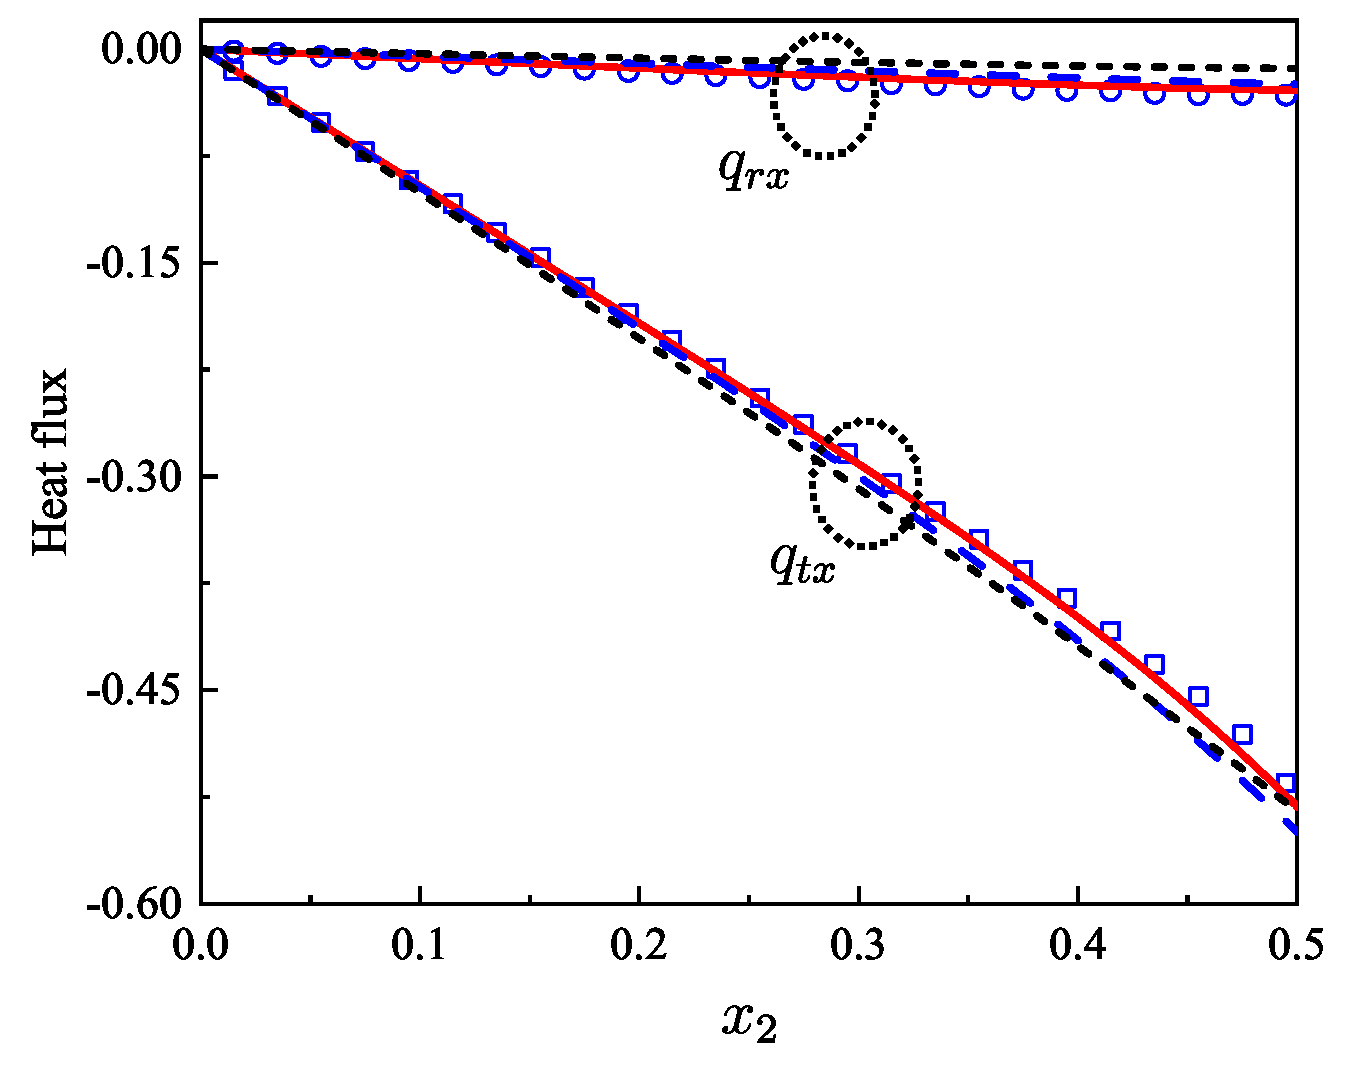
\includegraphics[scale=0.25,clip=true]{Fig/04CF6.eps}}
	\caption{ 
		平板库特流动中的密度、温度和垂直于流动方向的热流分布. 第一行和第二行的克努森数分别为 $\text{Kn}=0.1$ 和1. 基于对称性,另一半区域$-0.5\le{}x_1\le0$没有显示. 
	}
	\label{fig:Couette}
\end{figure*}



\subsubsection{正激波}






图~\ref{fig:nsw_n2_Ma7}给出马赫数为7的一维氮气正激波的结构. 空间坐标用激波上游的分子平均自由程$L=16\mu/5n\sqrt{2\pi{m}k_BT}$对其进行无量纲化,密度与温度通过 $ (Q-Q_u)/(Q_d-Q_u) $ 归一化,其中 $Q=n, T_t, T_r$, 下标$u$和$d$分别代表上游和下游的物理量. 所有动理学模型的密度分布均与DSMC计算结果大体上相符,只有ES-BGK模型给出的密度在波前稍低一些. Shakhov模型和ES-BGK模型的平动温度在波前存在“过早温升”现象,其中ES-BGK的平动与转动温度分布偏离最大,这是因为这两个模型方程的碰撞时间与分子速度无关. 而吴模型和DSMC中的碰撞时间都是分子速度的单调递增函数,因而得到最为接近的结果. 图~\ref{fig:nsw_n2_Ma7}(c,d)给出了压力与热流分布的计算结果, 可见吴模型与DSMC符合得非常好,而其它模型均存在显著误差,尤其是对比热流的分布.






\subsubsection{库特 流动}\label{sec:planar-couette-flow}

平板库特流动的上下两板温度相同,处在$x_2=L/2$的上板速度是$ v_w=v_m $,处在$x_2=-L/2$的下板速度相反. 图~\ref{fig:Couette} 给出各模型和DSMC的对比结果. 当$\text{Kn}=0.1$,所有动理学模型都给出了良好的密度分布. ES-BGK模型高估了平动温度和平动热流,却低估了转动热流. Rykov模型给出良好的温度和转动热流,却高估了平动热流. 吴模型跟DSMC的对比结果非常好. 当$ \text{Kn}=1 $,吴模型同样能给出与DSMC较为一致的结果. Rykov模型方程的密度分布与DSMC的结果稍有差别,在两板中心区域略低. ES-BGK模型的转动温度也略低于其他模型. 

\begin{figure*}[t]
	\centering
	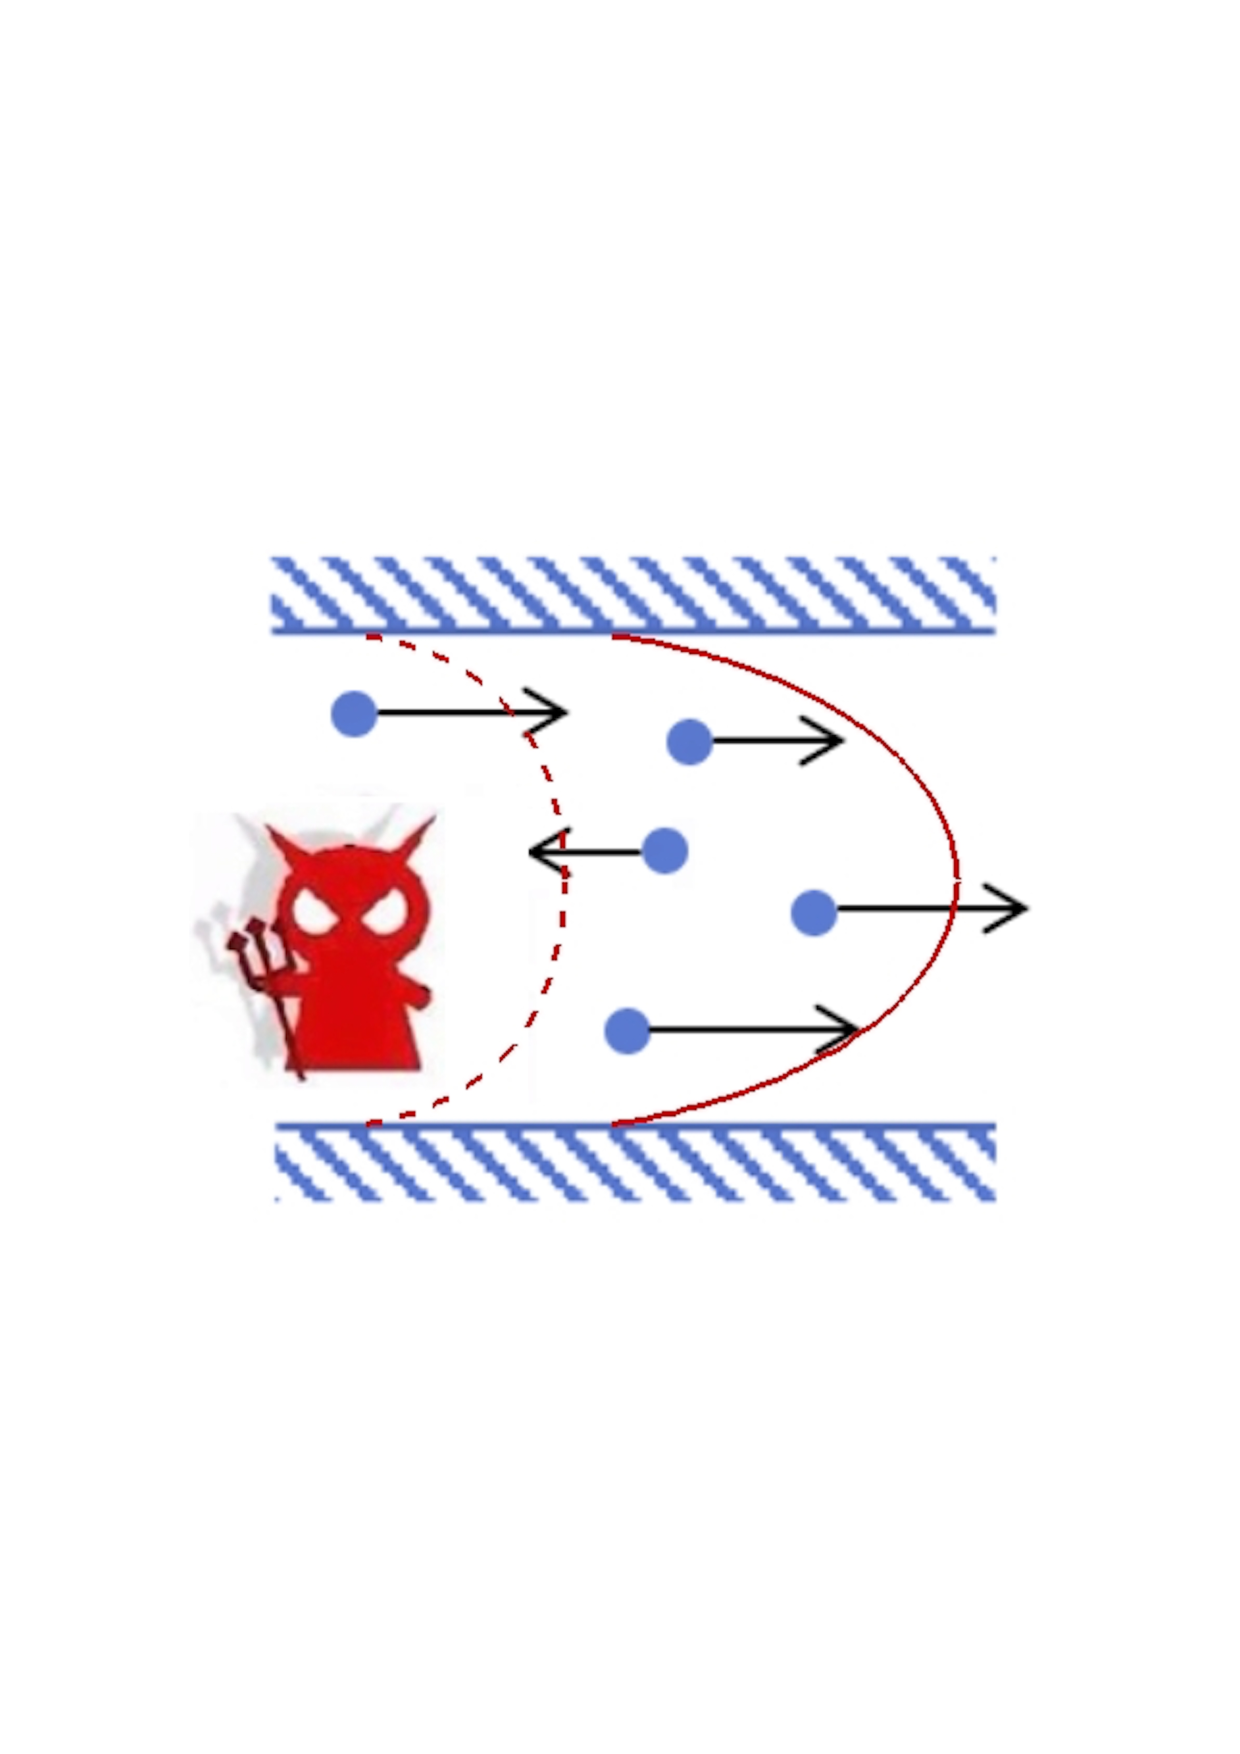
\includegraphics[scale=0.3,clip=true]{Fig/ThermalCreepDemon}\\
	\vskip 0.2cm
	{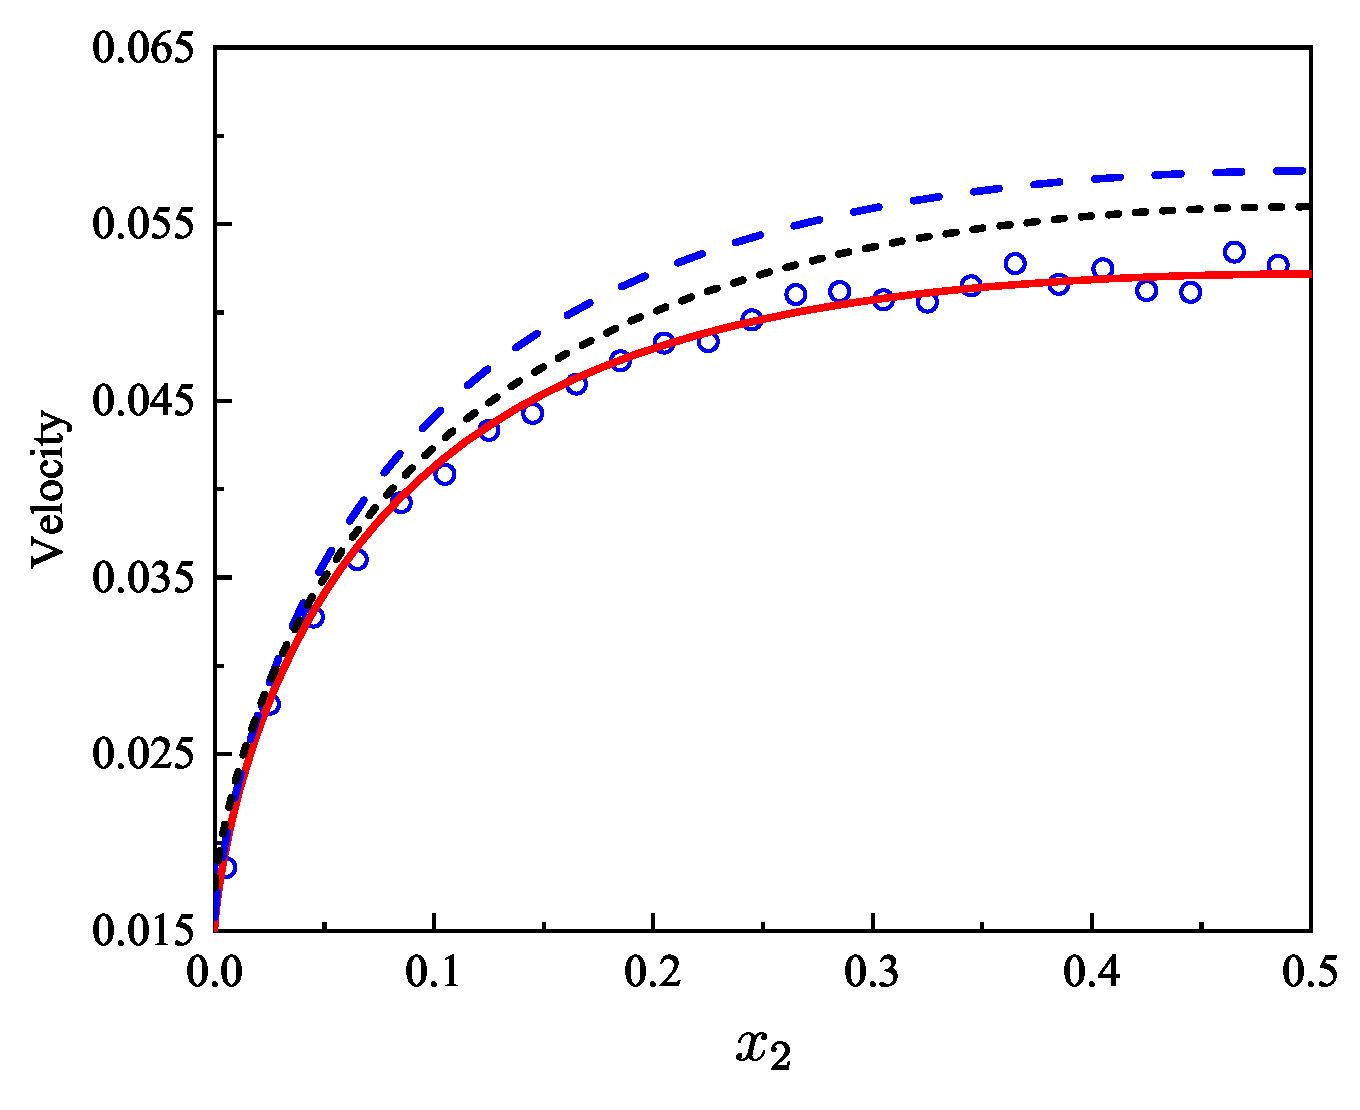
\includegraphics[scale=0.28,clip=true]{Fig/05TC1D1.eps}}\quad
	{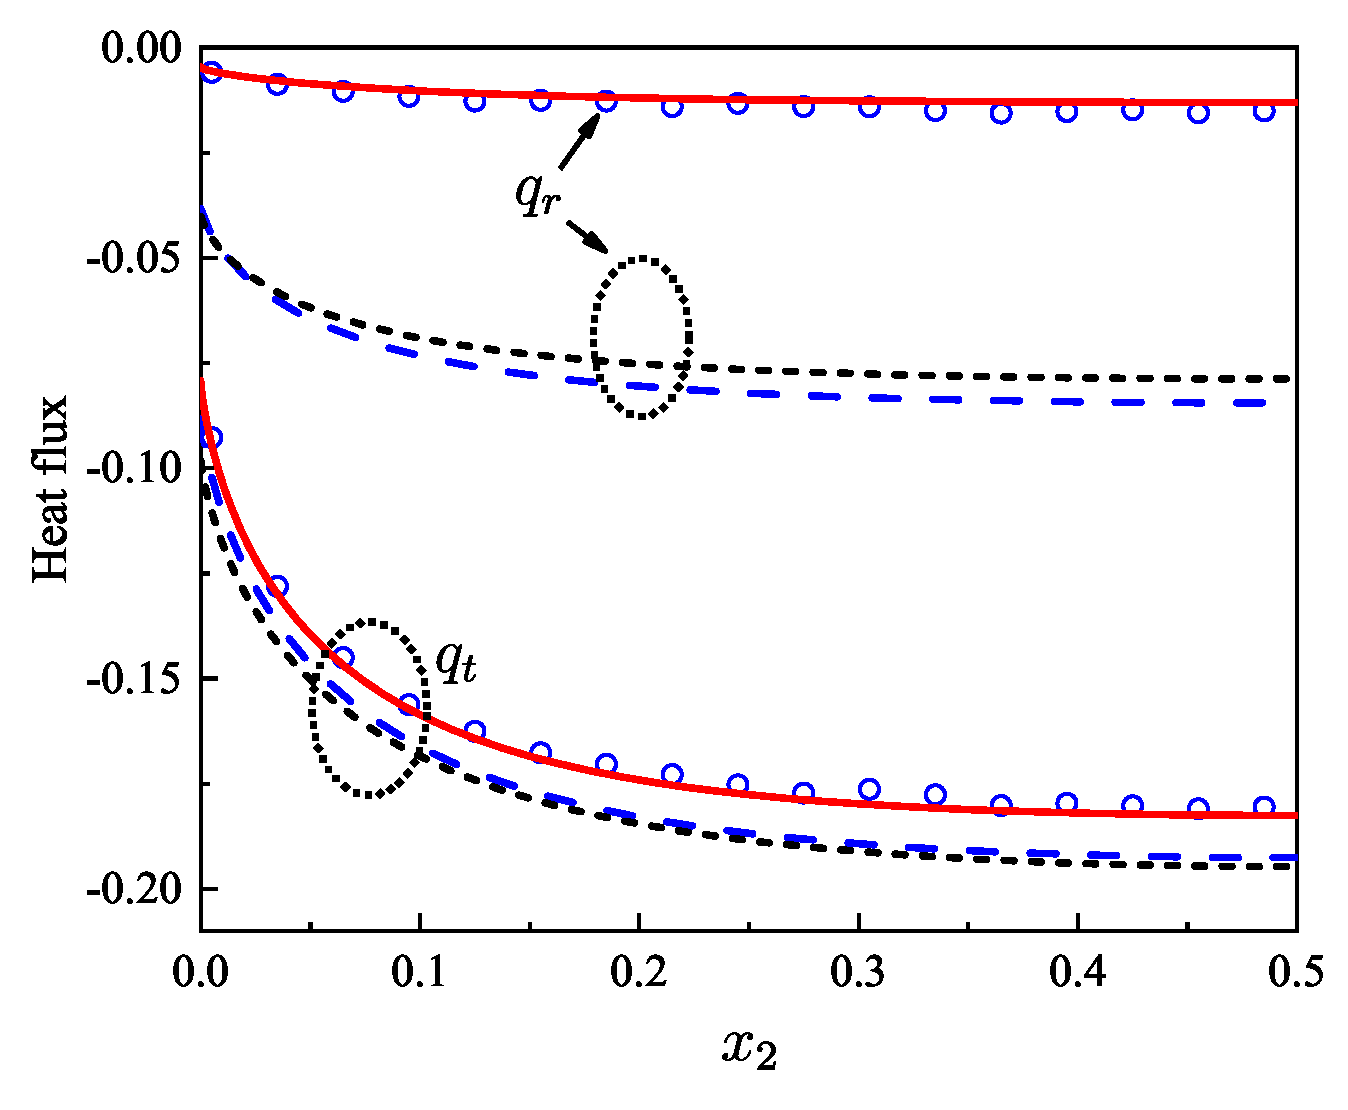
\includegraphics[scale=0.28,clip=true]{Fig/05TC1D2.eps}}\\
	\vskip 0.5cm
	{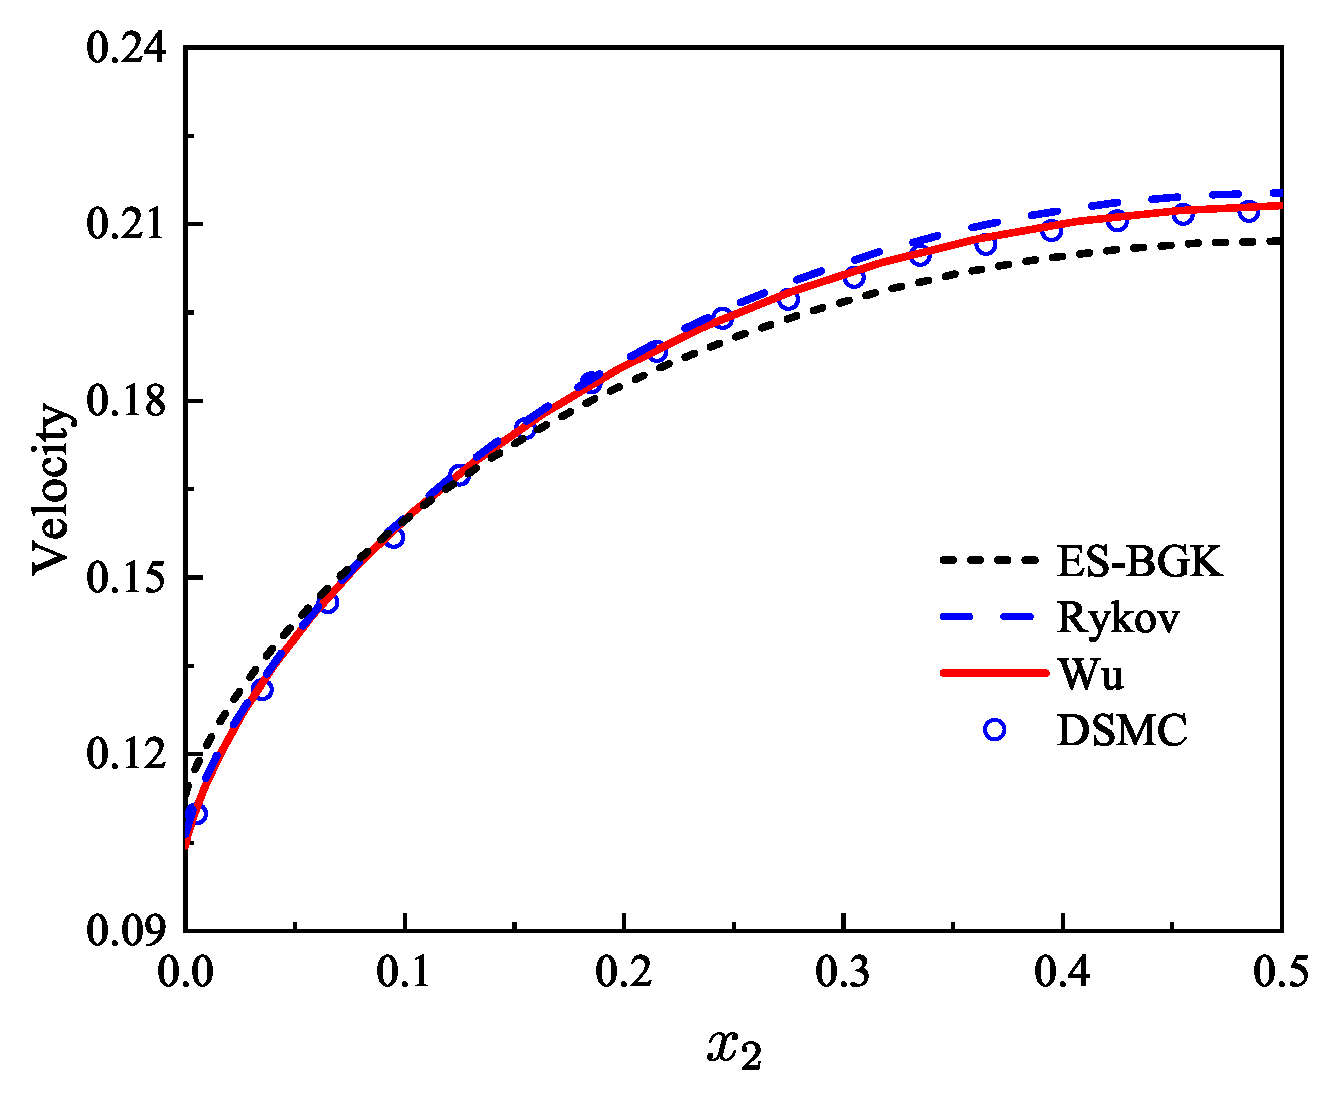
\includegraphics[scale=0.28,clip=true]{Fig/05TC1D3.eps}}\quad
	{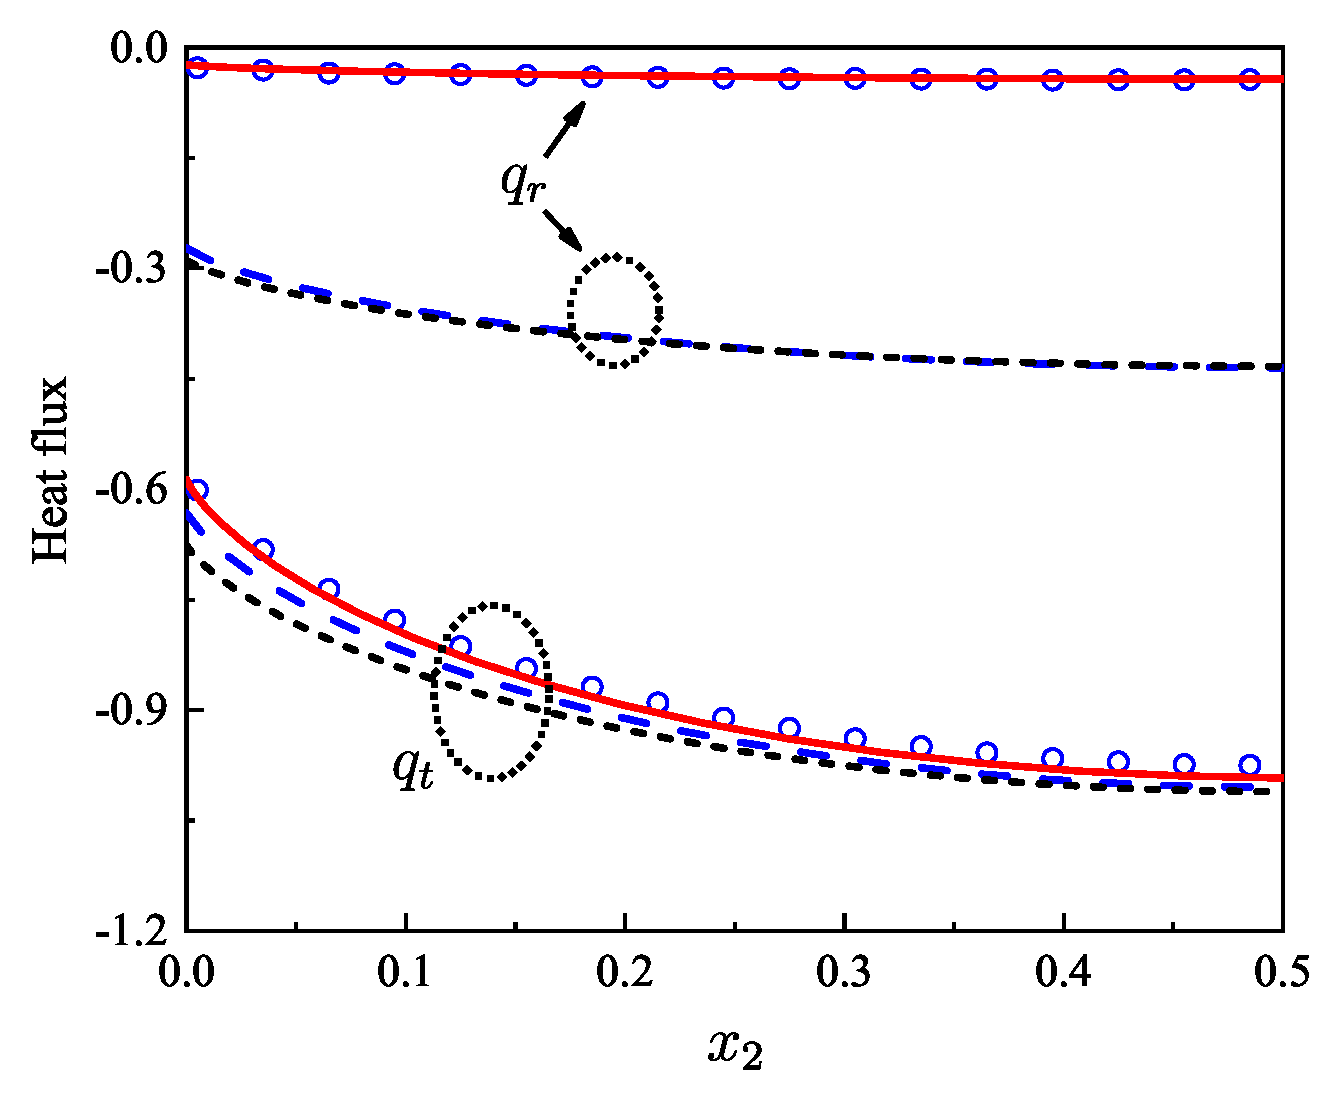
\includegraphics[scale=0.28,clip=true]{Fig/05TC1D4.eps}}
	\caption{ 
		麦克斯韦妖驱动下的稀薄气体热蠕动, 其中速度和热流均沿 $ x_1 $ 方向. 第二行和第三行图对应的克努森数分别为  $ \text{Kn}=0.1 $ 和1. 基于对称性,$0.5\le{}x_2\le1$的区域没有显示. \\
		Profiles of the vertical velocity and heat flux in the thermal creep flow driven by the Maxwell demon, where the Knudsen number in the second and third rows is $\text{Kn}=0.1$ and 1, respectively. Due to symmetry, the other half region $0.5\le{}x_2\le1$ is not shown.
	}
	\label{fig:TC1D}
\end{figure*}

\subsubsection{麦克斯韦妖驱动的微流动}

考察处在两平行静止的无限长平板间的分子气体,每个气体分子受到与其速度相关的外力的作用:
\begin{equation}
a_y=a_0\left(\frac{v^2}{v^2_m}-\frac{3}{2}\right),
\end{equation}
在此例中,取${2{a_0}{L}/{v^2_m}=0.0718}$,以保证系统仅略微偏离平衡态. 可以看出,当分子速率大于$\sqrt{3/2}v_m$时,其加速度为正,反之则为负. 因此该加速度可以看出是一种特殊形式的麦克斯韦妖,见图~\ref{fig:TC1D}. 


图~\ref{fig:TC1D}给出克努森数分别为0.1和1的模拟结果对比. 吴模型与DSMC非常符合,速度剖面与热流分布的最大误差仅为$ 2\% $. 值得注意的是,ES-BGK模型和Rykov模型的转动热流值远大于吴模型和DSMC的结果。其原因在于,这两个模型方程中的平动热流弛豫与转动热流弛豫相解耦,即$A_{tr}=A_{rt}=0$,即便热导率相近,但热弛豫系数的差别仍可导致显著的宏观量的差异。 这正说明了采用正确的热弛豫速率的重要性.





\begin{figure}[t]
	\centering
	\subfigure[]{\includegraphics[scale=0.5,clip=true]{Fig/06TC2D1.eps}} \\
	\subfigure[]{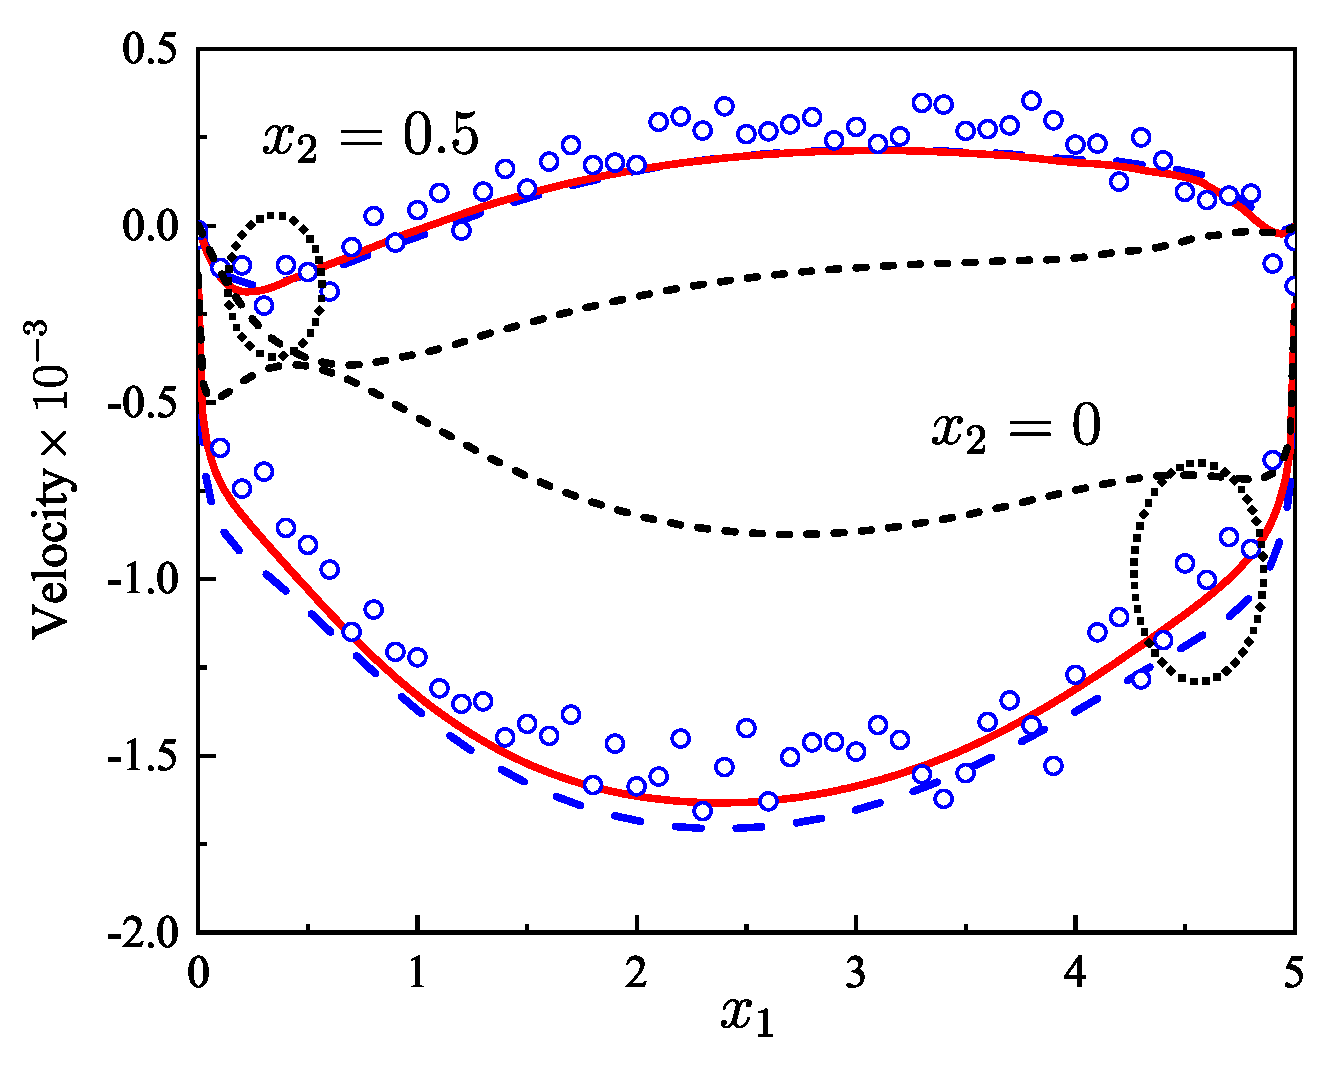
\includegraphics[scale=0.25,clip=true]{Fig/06TC2D2.eps}}
	\subfigure[]{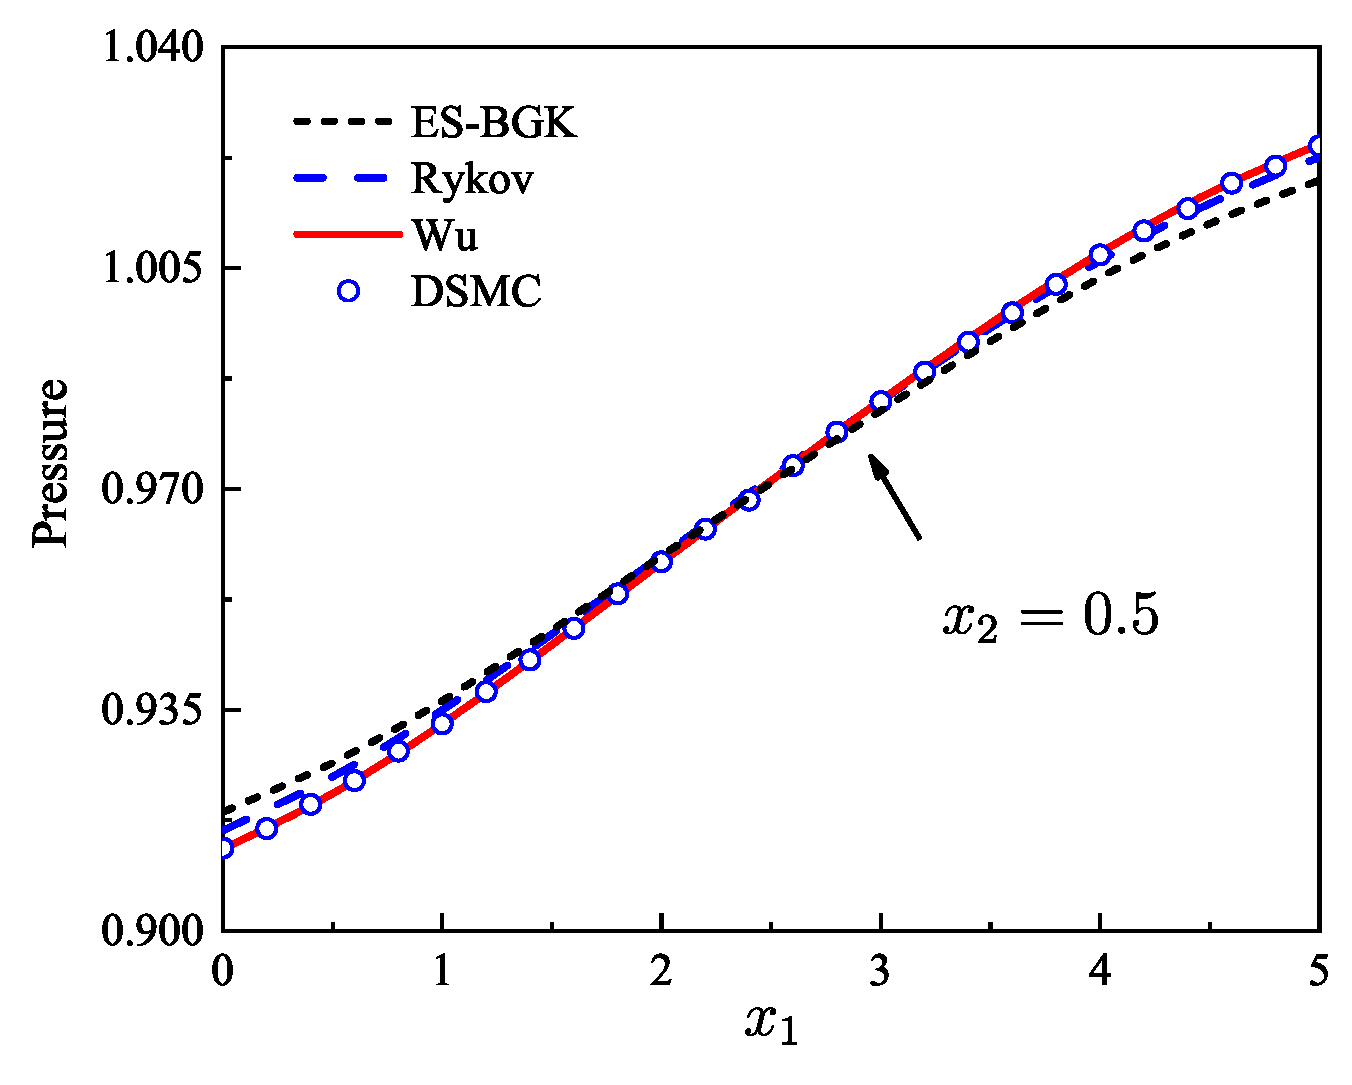
\includegraphics[scale=0.25,clip=true]{Fig/06TC2D3.eps}}
	\subfigure[]{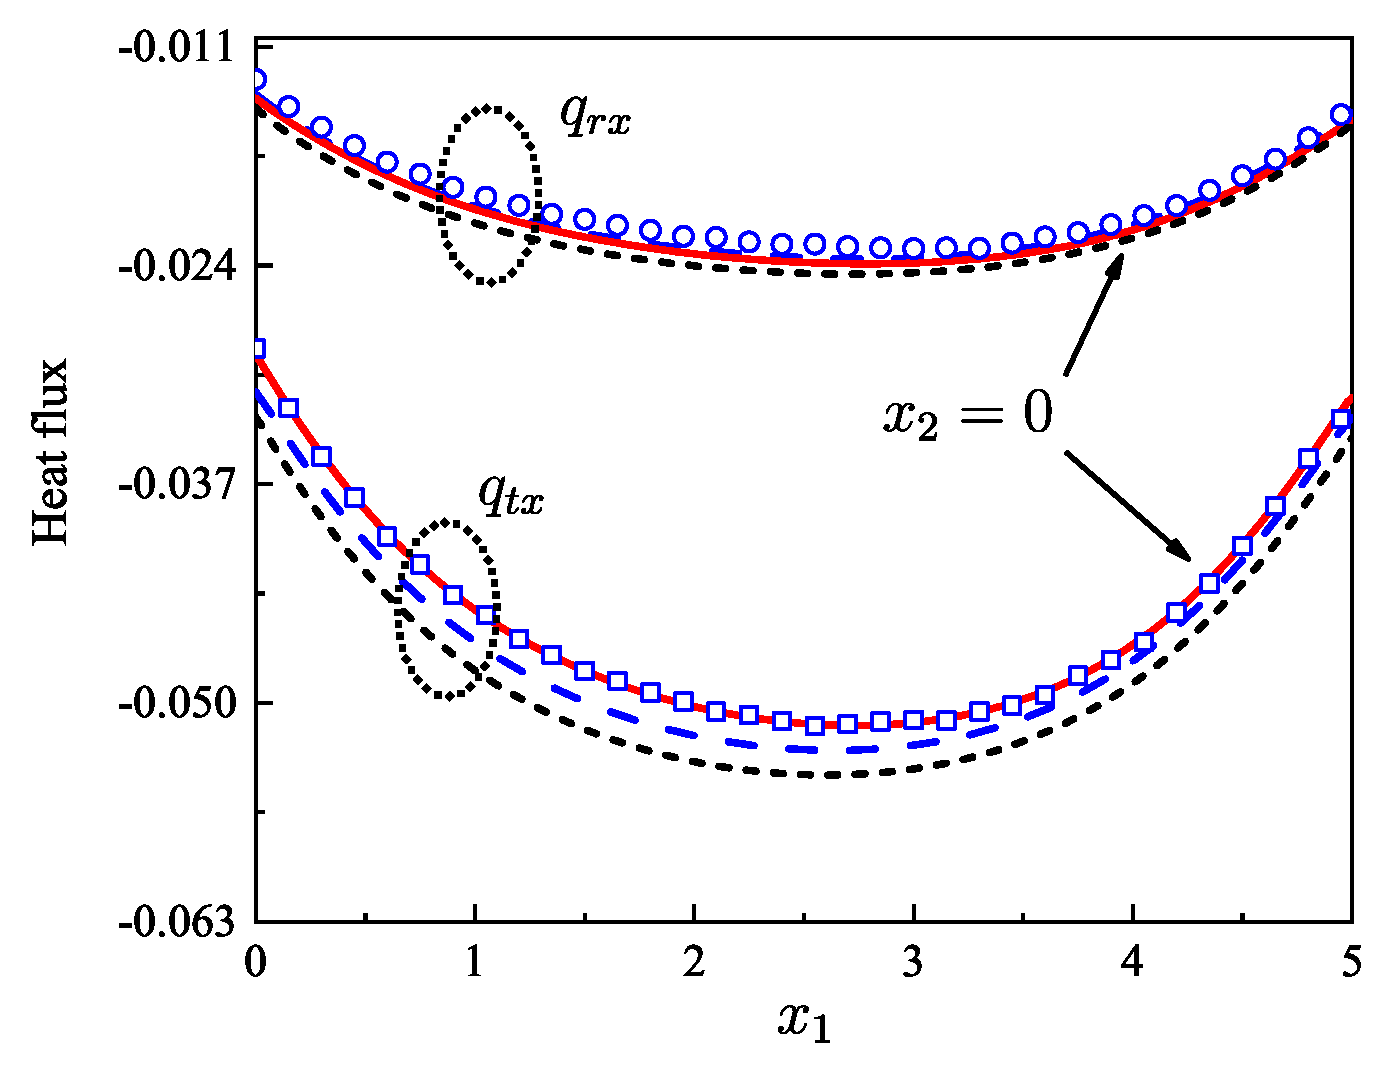
\includegraphics[scale=0.25,clip=true]{Fig/06TC2D4.eps}}
	\caption{克努森数为0.6的稀薄气体在二维方腔内的热蠕动.
		(a) 流场与 $ x_1 $ 方向的平动热流云图. (b) $ x_2=0, 0.5$ 处的速度剖面.(c) $x_2=0.5$ 处的正压力.(d)$x_2=0$ 处的平动和转动热流. \\
		Rarefied gas flow driven by temperature gradient in the solid walls. (a) The streamlines and the contour of translational heat flux in the $x_1$ direction. (b) Velocity profiles at $ x_2=0$ and 0.5. (c) The normal pressure at $x_2=0.5$. (d) The translational and rotational heat fluxes along the bottom wall.
	}
	\label{fig:TC2D}
\end{figure}







\subsubsection{封闭方腔中的热蠕动}

最后,考察二维封闭方腔内的热蠕动问题. 方腔宽度与高度比值为5,固定左板和右板的温度分别为 200~K 和 400~K,而上下两板的温度在此间线性分布. 由于此问题以 $x_2=0.5$ 为轴具有对称性,实际计算区域为方腔的下半部分. 取参考温度为300~K,参考长度为方腔高度,模拟克努森数为 $ \text{Kn}=0.6 $的气体流动.




图~\ref{fig:TC2D}中给出各个动理学模型方程与DSMC结果的比较. 吴模型的热流云图与速度剖面均与DSMC结果相符,而ES-BGK模型热流与速度剖面的解与DSMC的解有非常大的偏离,并且ES-BGK模型计算得到的中心涡更偏向右侧的高温区,且结构范围更小. 另外,Rykov模型在预测热流方面存在一定误差.


本节考察常用的气体动理学模型方程,Rykov模型、ES-BGK模型和吴模型,保证所有模型的剪切粘性、体积粘性和总热导率均与DSMC相同. 在吴模型中,通过调整热弛豫系数分量可以自下而上恢复所有的热导率分量. Rykov模型可以同时恢复正确的热导率分量,但是无法恢复所有的热弛豫系数,ES-BGK模型仅有一个参数自由度,用于调整总热导率,其热导率分量的比例不可调整. 数值结果表明:
\begin{enumerate}
	\item BGK类模型方程,能很好地模拟低速稀薄流动问题,而对于热导率起主导作用的传热问题,需选择能够分别恢复热导率分量的模型方程.
	
	\item 在热蠕动中,速度与热流结果取决于平动热导率,并且热弛豫速率分量对转动热流有影响.若BGK类型的模型方程不能独立调整热弛豫速率分量,则不适合用来研究热蠕动流动问题.
	
	\item 对于非平衡效应较强的正激波问题,即便BGK类模型方程能够同时恢复正确的热导率分量与部分热流弛豫速率,若碰撞频率不依赖与分子速度,在高马赫数下波前会有很明显的温度早起现象.
	
\end{enumerate}




\begin{figure*}[!t]
	\centering
	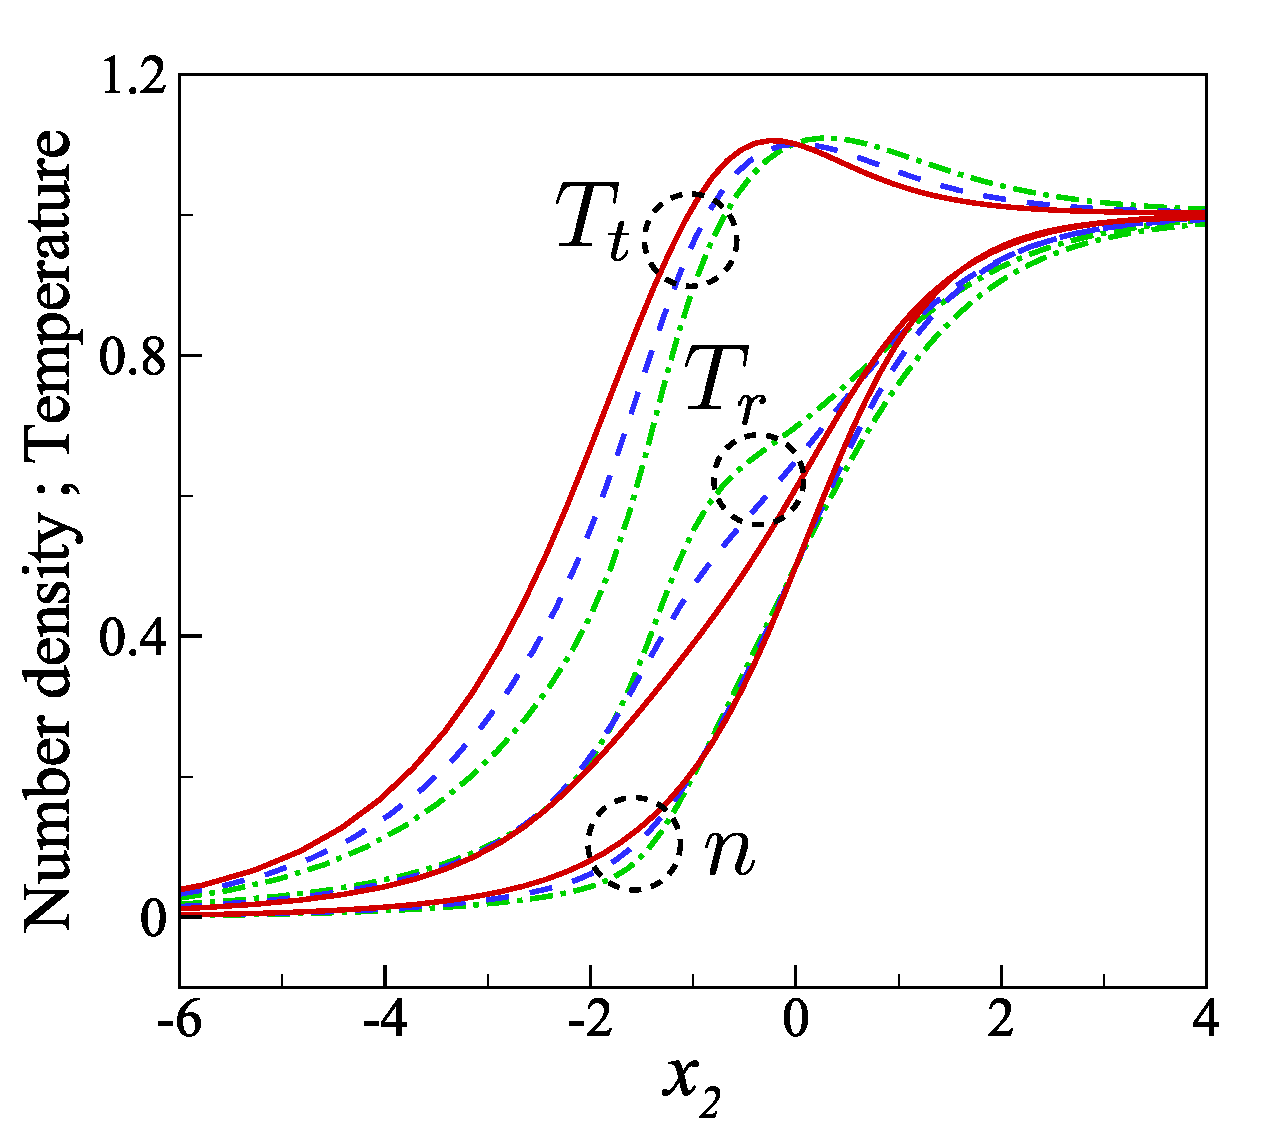
\includegraphics[scale=0.26,clip=true]{Fig/ShockWave_T_vf}\
	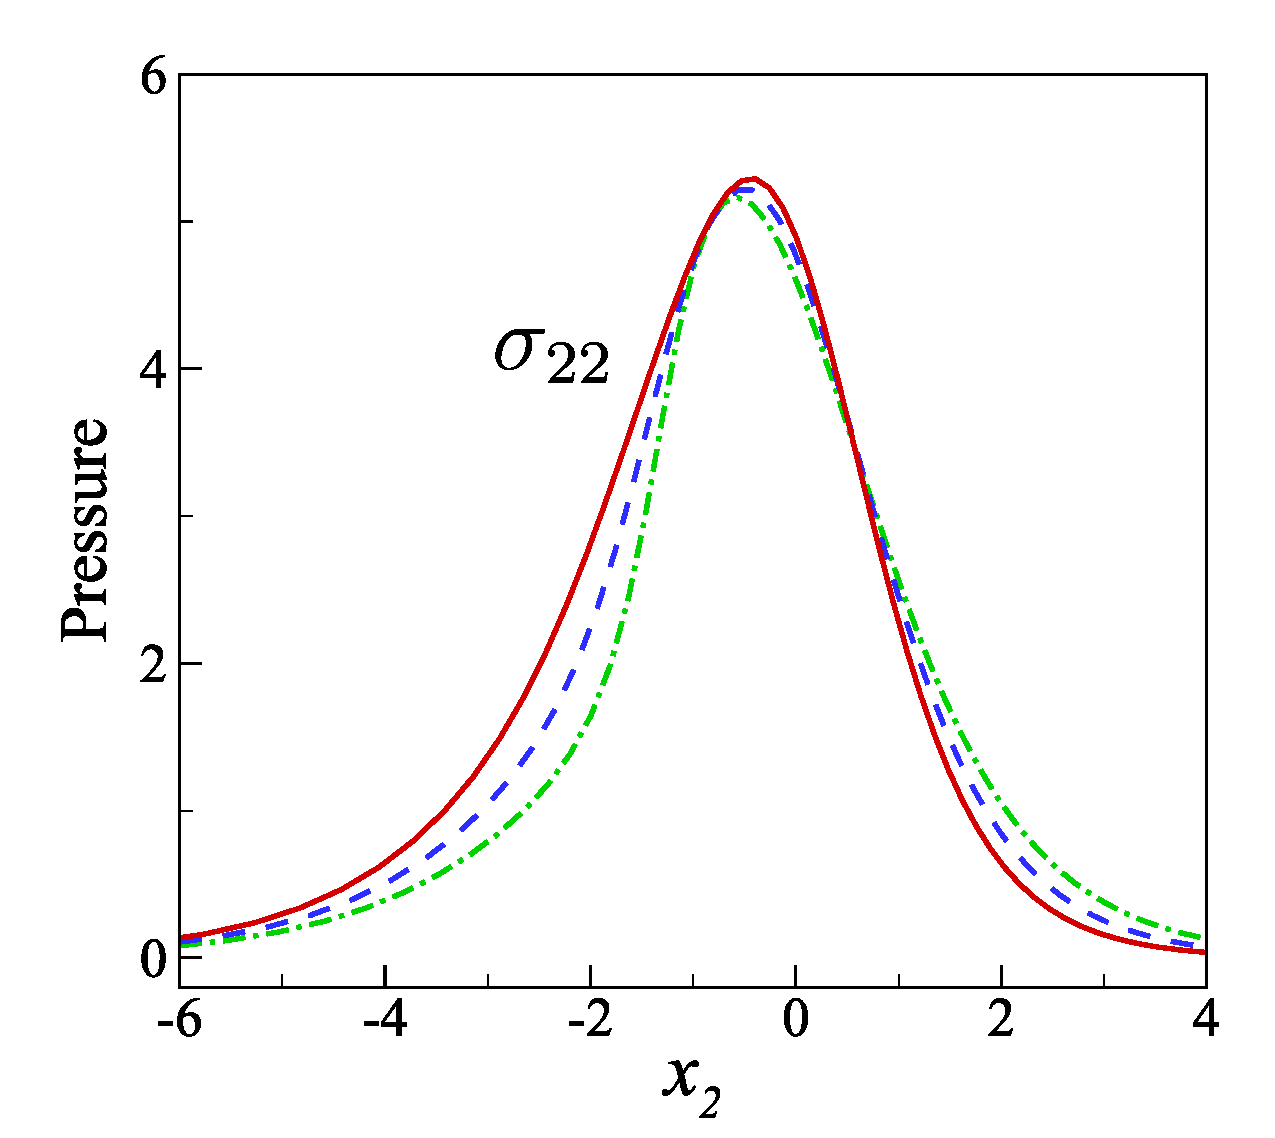
\includegraphics[scale=0.26,clip=true]{Fig/ShockWave_P_vf}\
	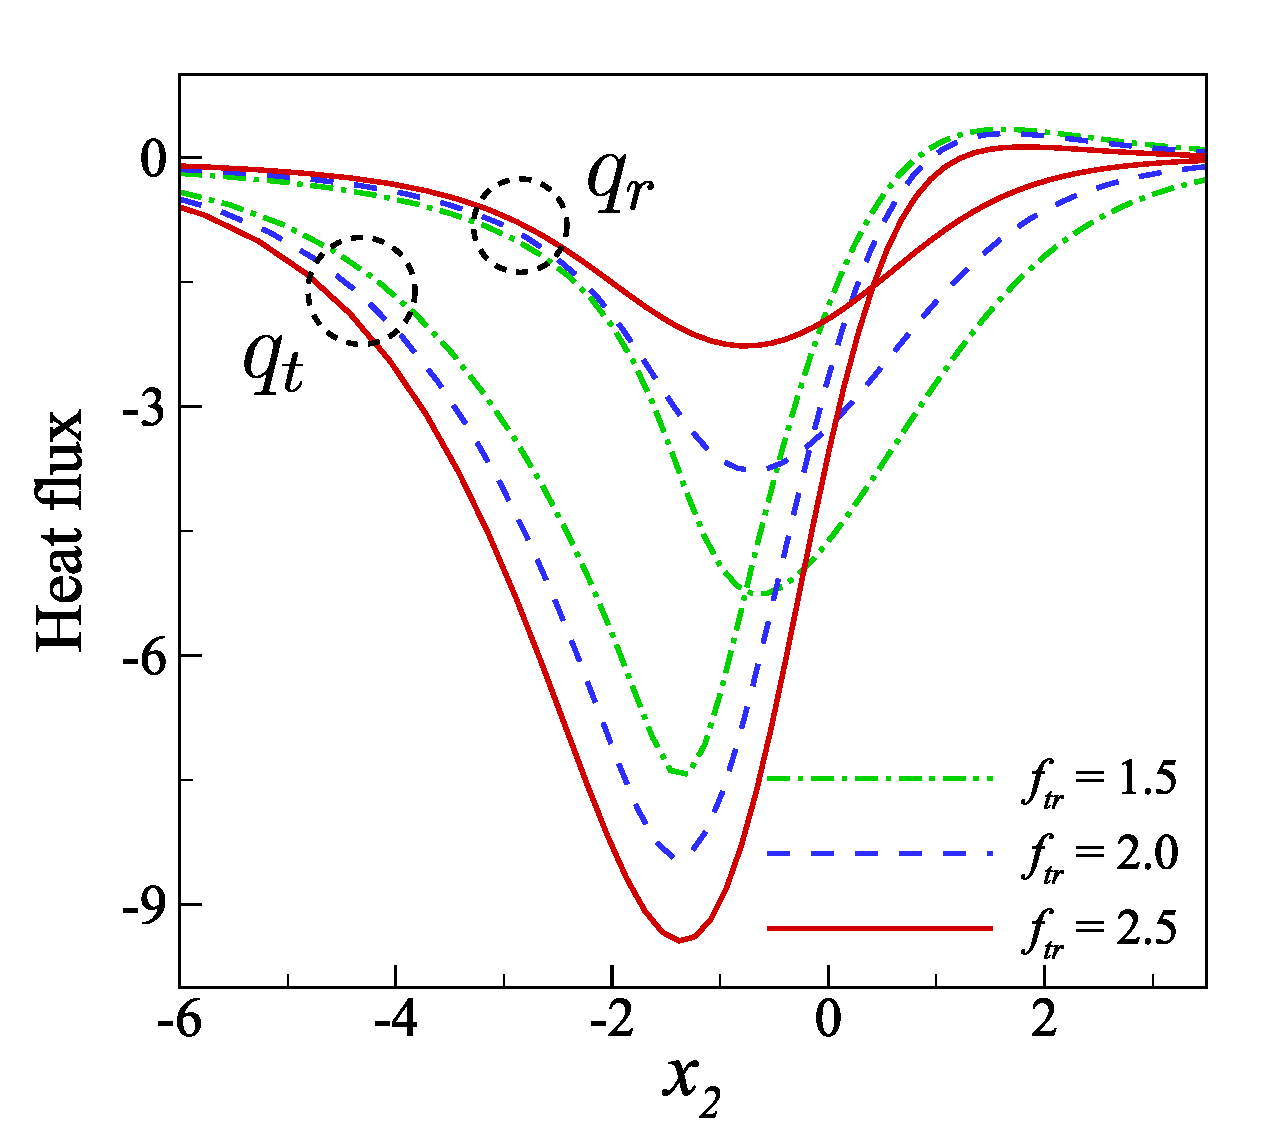
\includegraphics[scale=0.26,clip=true]{Fig/ShockWave_Q_vf}
	\caption{
		总Eucken因子不变时,不同平动Eucken因子对马赫数为4的正激波结构的影响. 图中数据来源于文献\cite{Li2021Uncertainty} \\
		Influence of the translational Eucken factor on the structure of normal shock wave with Mach number 4. The figures are from reference \cite{Li2021Uncertainty}.
	}
	\label{fig:shockwave_vary-f}
\end{figure*}

\section{热弛豫速率不确定度量化}\label{sec:uncertainty}

为了准确地预测稀薄分子气体的非平衡行为,气体动理学的建模过程应实现正确的剪切粘性、体积粘性以及平动、转动热导率. 分子气体的热导率比剪切粘性和体积粘性更加复杂,实验通常只能确定总热导率,但是难以其分辨平动与转动分量. 虽然在连续流极限下,气体动力学行为取决于气体粘性与总热导率,但是在稀薄流区,分子气体的平动与内能热导率可能对非平衡效应有各自不同的影响. %对分子气体热蠕动的实验研究表明~\cite{Mason1963JCP,gupta1970analysis,porodnov1978thermal,Loyalka1979Polyatomic},即使在压力梯度为零的情况下,气体也会自发从低温区移动至高温区,质量流量与平动热导率相关,而不是与总热导率相关.








\begin{figure*}[t]
	\centering
	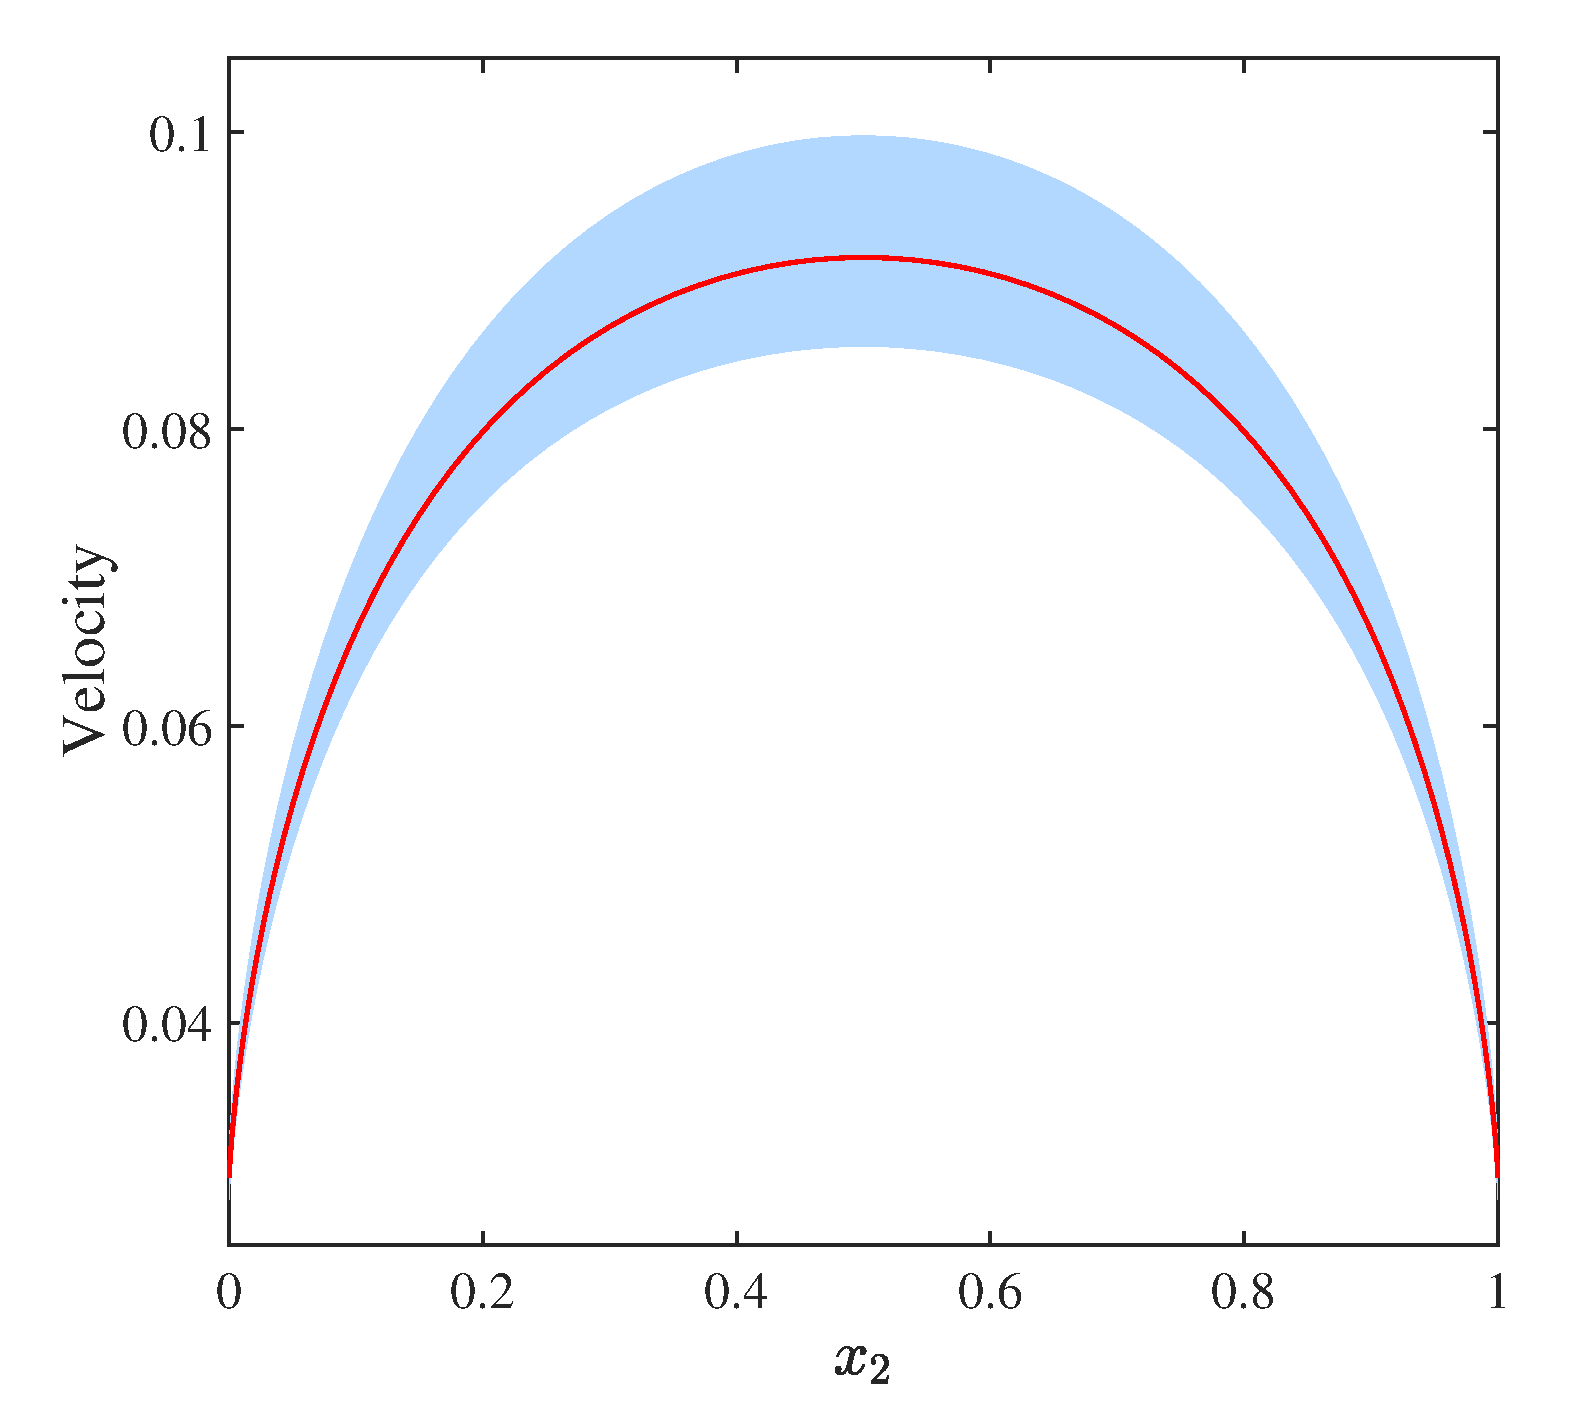
\includegraphics[scale=0.245,clip=true]{Fig/Creep_u_vA}\quad
	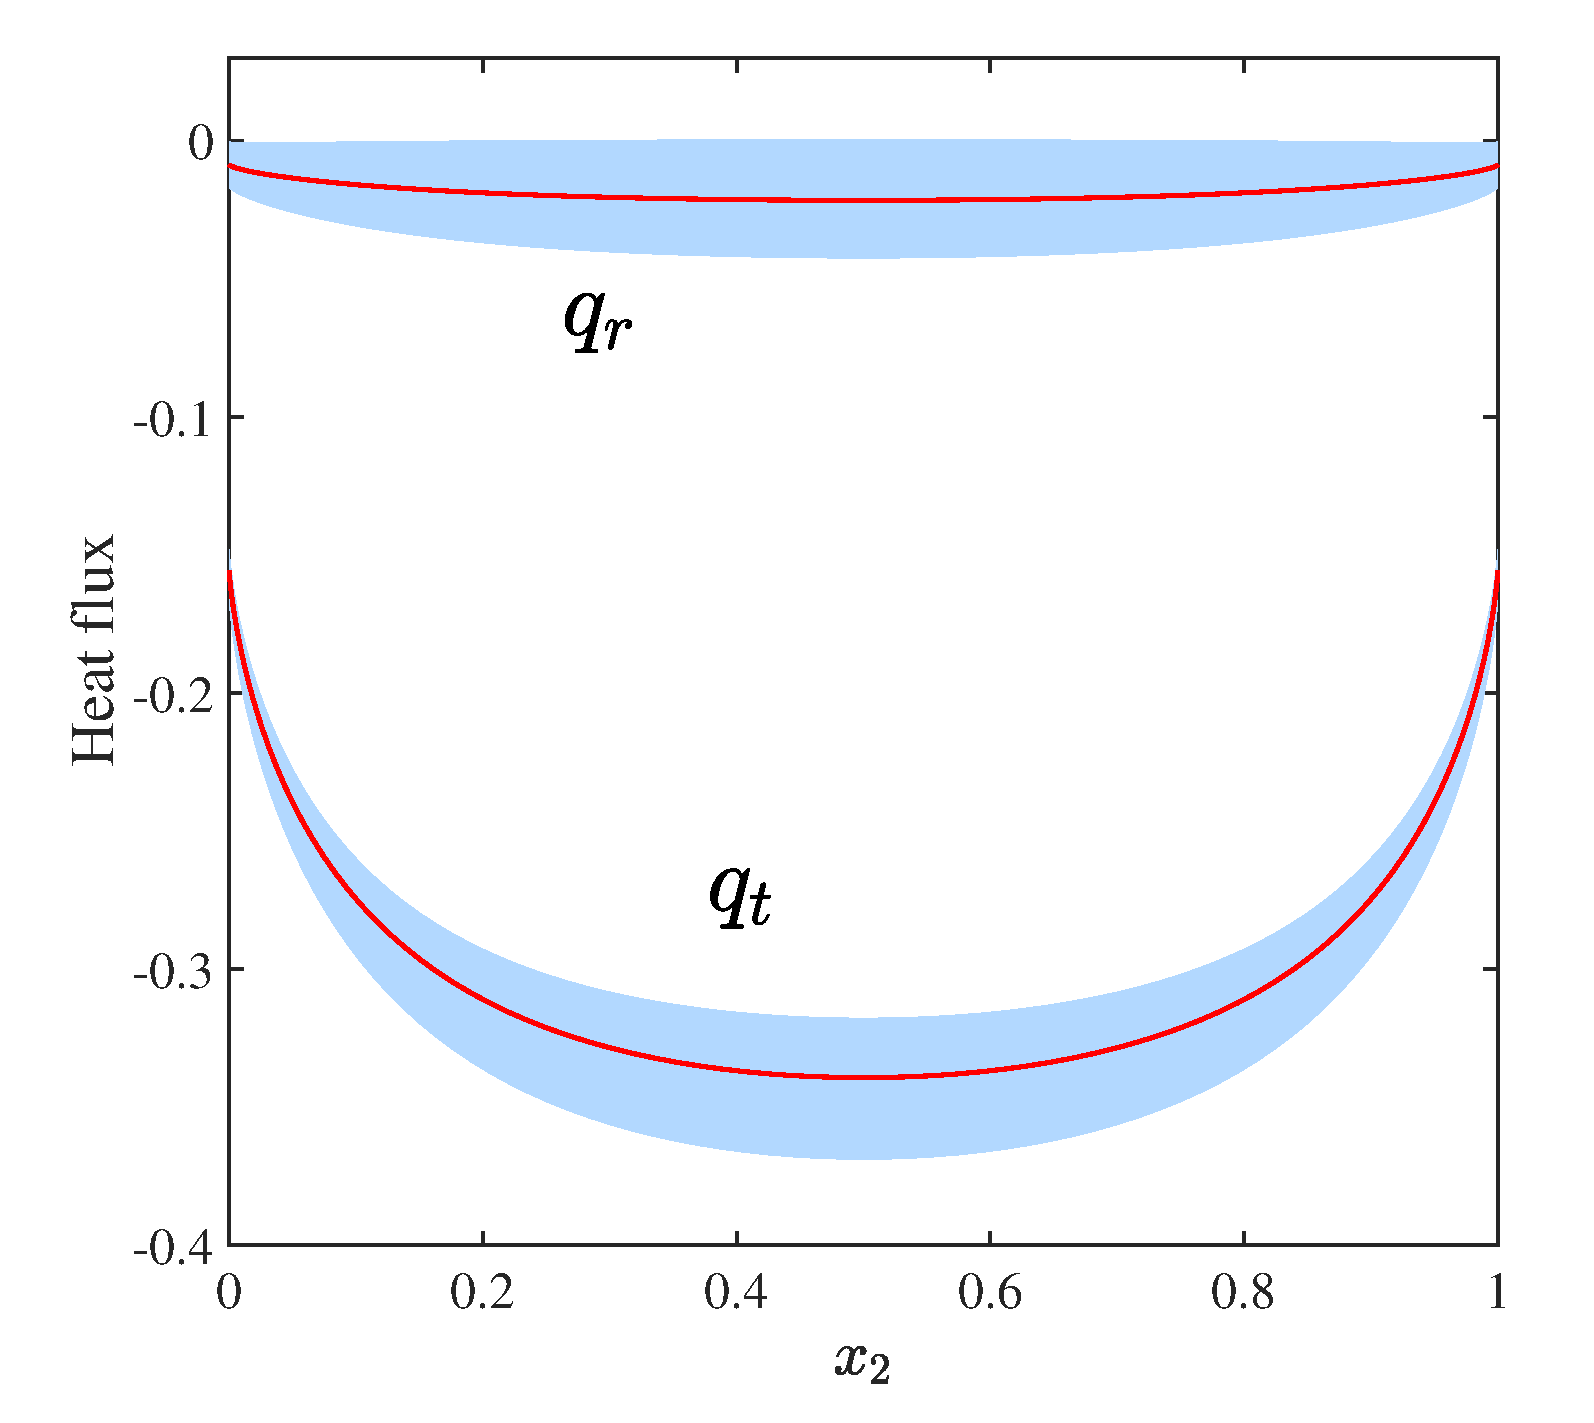
\includegraphics[scale=0.245,clip=true]{Fig/Creep_Q_vA}\\
	\vskip 0.5cm
	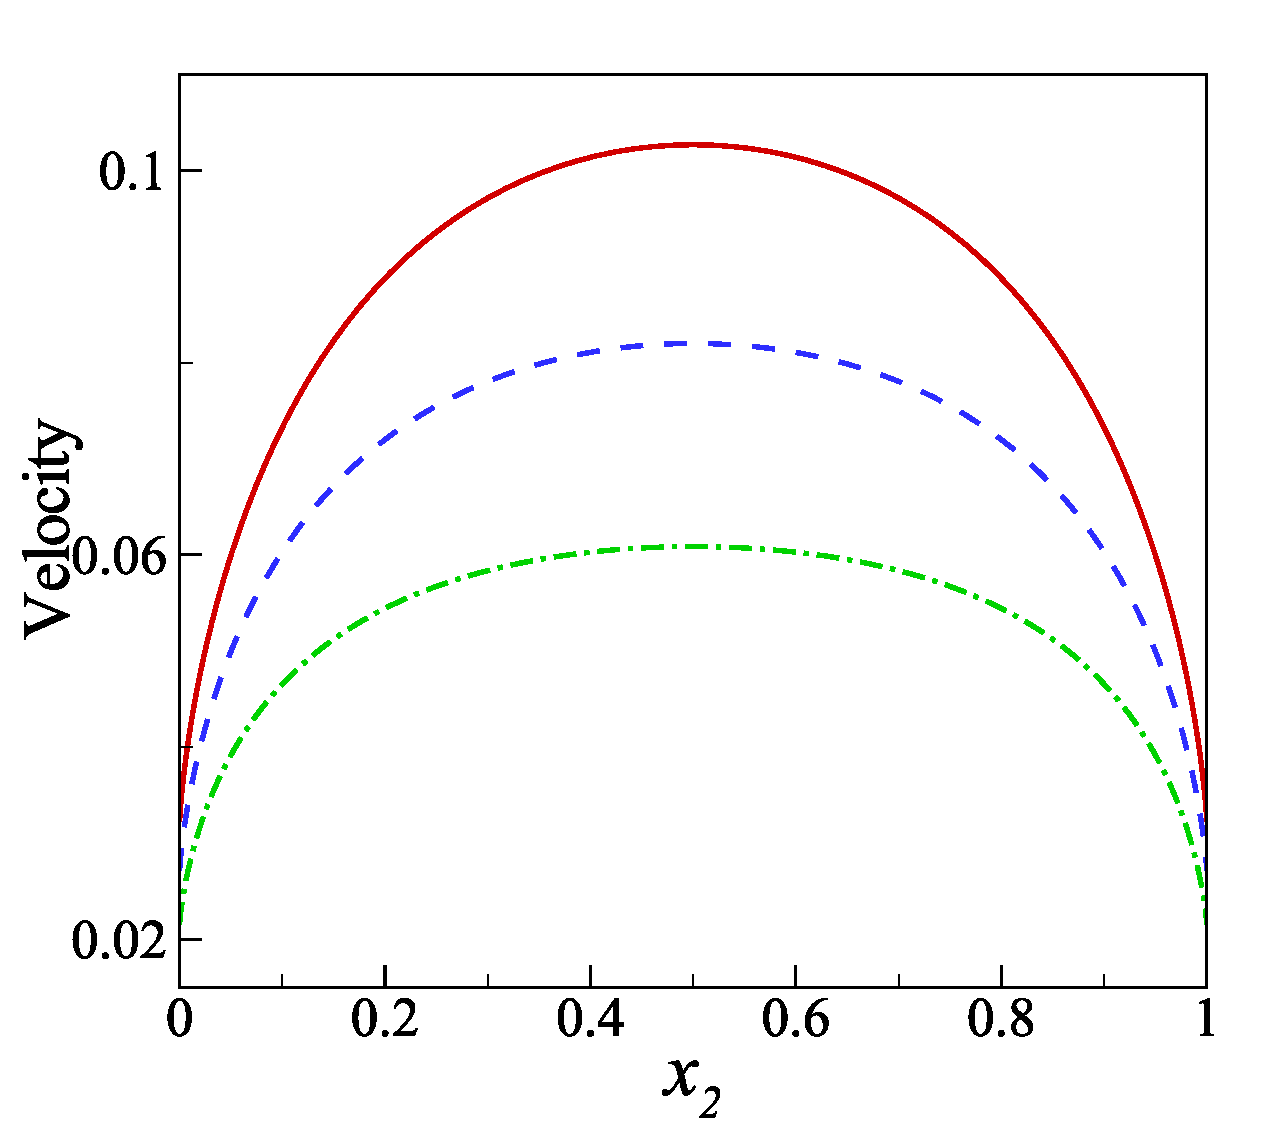
\includegraphics[scale=0.30,clip=true]{Fig/Creep_u_vf} \quad
	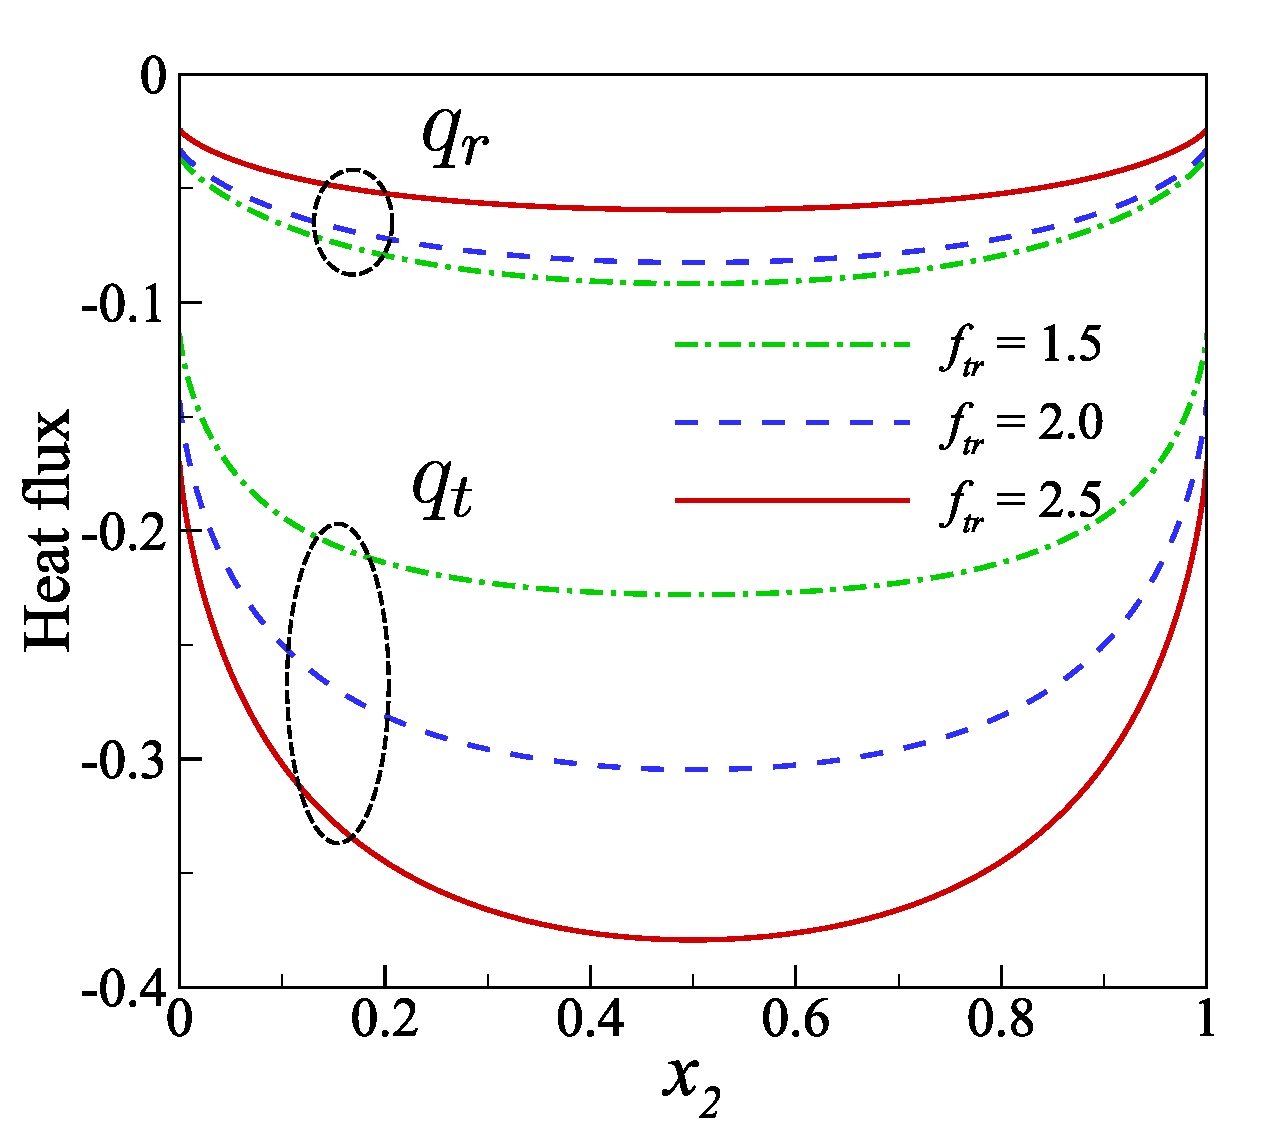
\includegraphics[scale=0.30,clip=true]{Fig/Creep_Q_vf}
	\caption{
		(第一行) 热流弛豫速率对麦克斯韦妖驱动的热蠕动速度和热流分布的影响. 吴模型中改变热弛豫速率的结果对比. 红色实线对应的 ${\bf{A}}$ 数值来自于DSMC,蓝色阴影部分来自吴模型计算结果,对应的取值范围为 ${A_{rt}}\in[-0.3124,0.0]$、${A_{tr}}\in[-0.1250,0.0]$. 其余参数为 $\text{Kn}=0.2$, $f_{tr}=2.365$ 以及 $f_{rot}=1.435$. 
		(第二行) 	总Eucken因子${f_{u}}$ 保持不变,改变平动Eucken因子的结果对比. $\text{Kn}=0.2$. 图中数据来源于文献\cite{Li2021Uncertainty}\\
		(First row) Influence of the thermal relaxation rates in the creep flow driven by the Maxwell demon. Red solid lines are the results with ${\bf{A}}$ extracted from DSMC, blue shade region shows the results from the kinetic model~\eqref{Wu_model}, with ${A_{rt}}\in[-0.3124,0.0]$ and ${A_{tr}}\in[-0.1250,0.0]$. Other parameters are $\text{Kn}=0.2$, $f_{tr}=2.365$ and $f_{rot}=1.435$. 
		(Second row)  Influence of the translational Eucken factor, while  ${f_{u}}$ is fixed. The Knudsen number is $\text{Kn}=0.2$. The figures are from reference \cite{Li2021Uncertainty}.
	}
	\label{fig:thermalCreep_vary-A}
\end{figure*}



上文的算例表明,热弛豫速率在稀薄气体流动中也起着重要作用. 尽管在DSMC和其他分子气体动理学模型中~\cite{Morse1964,holway1966new,Rykov,Gorji2013},已有大量关于温度弛豫效应~(与体积粘性相关)的研究工作,却从未有过关于热弛豫速率矩阵 $\bf{A}$ 对稀薄气体非平衡效应的影响的相关研究. 通过实验可以直接测量总热导率,并且在某些情况下,还可以提取平动热导率~\cite{Mason1963JCP,gupta1970analysis,porodnov1978thermal,Wu2020JFM}. 然而,根据公式~\eqref{relax_flux},弛豫系数矩阵 $\bf{A}$ 中至少有两个元素不能确定,即不同的系数矩阵$\bf{A}$可以对应一致的热导率及其分量。因此有必要量化在输运系数都一致的前提下,由系数$\bf{A}$的变化所带来的宏观量的不确定性.


在DSMC中,因碰撞模型的原因,固定体积粘性后,热弛豫系数也随之确定. 在吴模型中,可以通过独立修改 ${A_{ij}}$ 以量化热弛豫系数的影响. 上文已验证吴模型的准确性,这里我们使用吴模型来量化这种不确定性. 首先,在约束 ${f_{tr}}$ 和 ${f_{rot}}$ 不变的前提下修改 ${A_{ij}}$, 以研究热弛豫速率的影响. 其次,在保持总热导率不变前提下,通过改变 ${f_{tr}}$ 和 ${f_{rot}}$来量化热导率分量的影响.



\subsection{正激波}


给定 ${f_{tr}}$ 和 ${f_{rot}}$,即体系中所有的热导率分量都被确定,若此时其余的输运系数也保持不变,则称此系统为宏观意义上的确定系统. 然而,不同的 ${A_{ij}}$  的选择将可能导致结果的不确定性. 

考察一维正激波问题,${A_{tr}}$、 ${A_{rt}}$的取值范围分别为 $ [-5/(6Z),0] $ 和 $[-1/(3Z),0] $, 而 ${A_{tt}}$ 和 ${A_{rr}}$ 的值根据公式~\eqref{relax_flux}调整,以保持 ${f_{tr}}$ 和 ${f_{rot}}$ 不变. 在DSMC中非对角线元素为 $A_{tr}=-0.201, A_{rt}=-0.059$,本例中,给定 ${Z=2.6671}$,${A_{rt}}$ 和 ${A_{tr}}$ 的最小值分别为 $-0.3124$ 和 $-0.1250$, 数值大小约为DSMC对应参数的 一到两 倍. 我们发现,热弛豫系数 ${\bf{A}}$ 的变化导致转动温度和转动热流稍有变化,而对密度、速度和应力偏量 几乎没有影响.


接着,我们保持总热导率不变,且选择$A_{tr}=-5/(6Z), A_{rt}=-1/(3Z)$, 研究热导率分量的改变对流动的影响. 图~\ref{fig:shockwave_vary-f}展示了马赫数为4时,不同平动 Eucken 因子 下吴模型的数值结果. 在实际中,较小数值的平动Eucken因子 $f_{tr}$ 是可能存在的,特别是在极性气体中,真实的平动Eucken因子可能远小于 $ 2.5$. 例如,水的平动Eucken因子为 $f_{tr}=1.78$,甲醇分子~\cite{mason1962heat}的平动Eucken因子为 $f_{tr}=0.41$.  从对比中可以看出,所有的宏观量都随$f_{tr}$改变而有明显的变化. 首先,较大的${f_{tr}}$使得平动温度更快上升到其最大值,并在波后更快趋于下游温度,对于应力偏量和总热流也有相同的趋势. 其次,${f_{tr}}$变化所导致的转动温度变化则集中于激波结构的中心处,较小的${f_{tr}}$导致更高的转动温度. 最后,较大的${f_{tr}}$使得密度升高更快.

由此,在正激波问题中,由热弛豫系数$\bf{A}$的变化引起的不确定性较小,而热导率分量的变化则会带来显著的不确定性。例如, ${f_{tr}=1.5}$ 的转动热流大约是 ${f_{tr}=2.5}$的两倍,几乎与平动热流相当.

而对于由不同热弛豫系数引起的不确定性,图中~\ref{fig:shockwave_vary-A}矩阵 ${\bf{A}}$ 给总热流带来的不确定性仅为 ${7.4\%}$.





\subsection{麦克斯韦 妖驱动的微流动}\label{Maxwell demon}




使用正激波算例中的同一系列矩阵 ${\bf{A}}$,并使$f_{tr}$ 和 $f_{rot}$ 均保持不变,来考察麦克斯韦妖驱动的微流动中,热弛豫系数对流动速度和热流的影响. 图~\ref{fig:thermalCreep_vary-A}第一行图片数据为 $\text{Kn}=0.2$ 的结果. 可以看出,不同于正激波问题,此问题中不同热弛豫系数 ${\bf{A}}$ 对应的流动速度与热流有相当明显的差别. 流动速度和平动热流的最大相对不确定性分别为 $16.7\%$ 和 $17.6\%$. 同时可以看出,流动的中间区域出现了较大的不确定性,而壁面附近的速度滑移与热流几乎不变.


\begin{figure}[t]
	\centering
	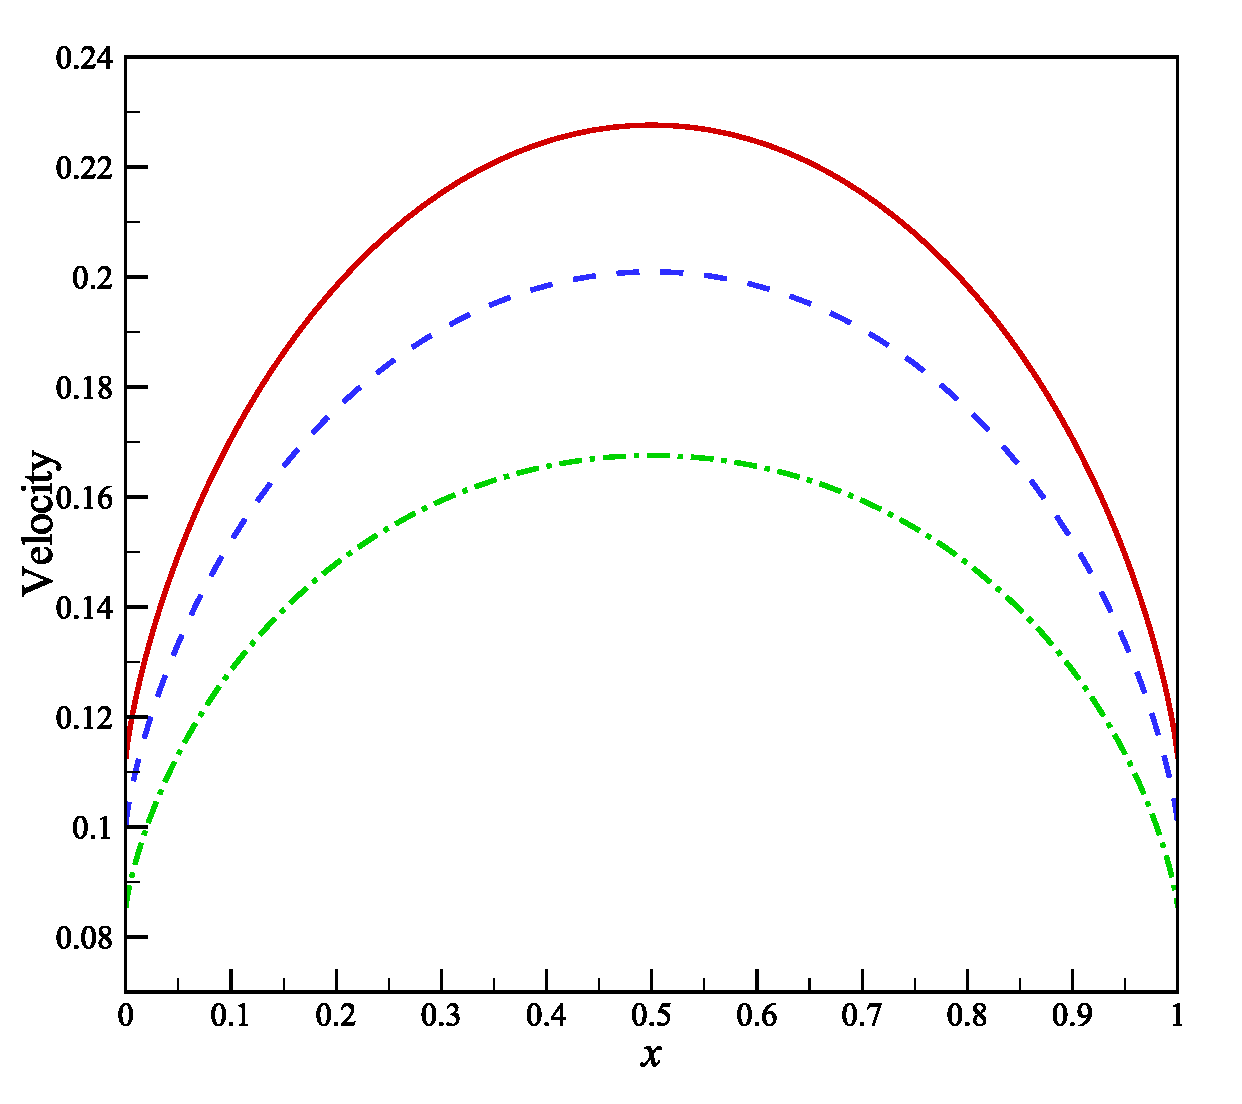
\includegraphics[scale=0.3,clip=true]{Fig/ThermalCreep_U_vf} 
	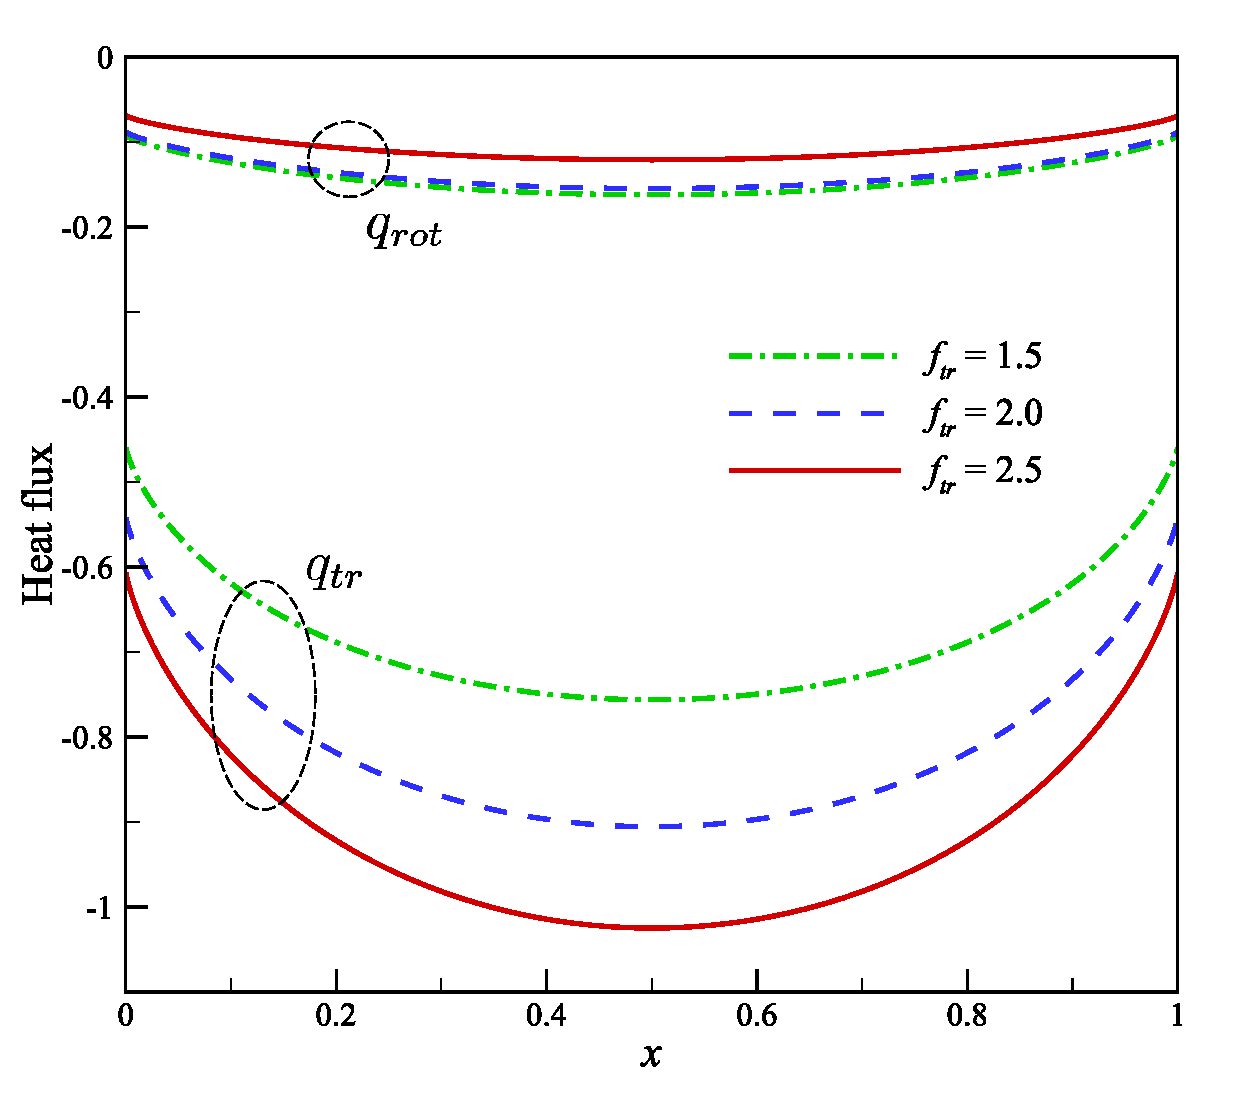
\includegraphics[scale=0.3,clip=true]{Fig/ThermalCreep_q_vf}
	\caption{
		在麦克斯韦妖驱动的热蠕动中,不同平动Eucken因子的结果对比. 总Eucken因子${f_{u}}$ 保持不变,$\text{Kn}=1$.\\
		Influence of the translational Eucken factor in the creep flow driven by the Maxwell demon. All cases have the same ${f_{u}}$ and ${Kn=1}$, while $f_{tr}$ for green dash-dot, blue dashed, and red solid lines are 1.5, 2.0, and 2.5, respectively.
	}
	\label{fig:thermalCreep_vary-f}
\end{figure}

为进一步研究平动Eucken因子的影响,考察Eucken因子 ${f_{tr}=1.5, 2.0, 2.5}$ 的算例,其余参数为$\text{Kn}=0.2$,$f_u=1.993$, $A_{tr}={-5/6Z}$,$A_{rt}={-1/3Z}$. 如图~\ref{fig:thermalCreep_vary-A}第二行图片数据所示,速度曲线与平动热流随着平动Eucken因子的变化而剧烈变化. ${f_{tr}=2.5}$ 时的流动速度和热流比 ${f_{tr}=1.5}$ 时增加了大约 ${68\%}$ . 在第一行图中,在确定的 $ f_{tr} $ 下,壁面速度滑移与热流不受平动Eucken因子的影响. 而在第二行图中,速度与热流依赖于平动Eucken因子,例如, 壁面附近的速度与热流均与 ${f_{tr}}$ 呈正相关. 这说明,在此问题中,平动Eucken因子 ${f_{tr}}$ 起主导作用.


平动Eucken因子在此问题中的重要性可得到如下解释:从方程~\eqref{relax_flux} 可以看出,热弛豫系数 ${A_{tr}}$ 和 ${A_{rt}}$ 与 平动能与转动能之间的能量交换有关. 当 ${A_{tr}}$ 与${A_{rt}}$为零时,平动热流与转动热流的弛豫过程互相解耦. 例如,更多的计算结果显示,在${A_{rt}=0}$ 的情况下,转动热流恒为零. 这是因为麦克斯韦妖驱动的热蠕动流动中,外力项仅能直接影响平动能,而转动能和热流则需通过能量交换才能发生改变,具体取决于${A_{tr}}$, ${A_{rt}}$ 和 $Z$. 由于矩阵的非对角元素 相对于其他元素为小量,这导致 $q_{rot}\approx0$,而平动效应 ($q_{tr}$ 或者 $f_{tr}$)占主导.



\section{确定热流弛豫速率的方法}\label{determine_uncertainity}

上文的研究结果揭示了热流弛豫速率不确定性对稀薄气体流动的影响, 因此有必要通过获取并使用正确的相应系数,来减少或消除模型的不确定性. 我们认为可以尝试以下两种方法.

\subsection{分子动力学模拟}

从物理上来说,只要知道了分子间的相互作用势,根据牛顿第二运动定律,就可以通过分子动力学方法模拟气体的行为. 由此,输运系数能够通过Green-Kubo公式获得\cite{Green1954,Kubo1957Japan}:
\begin{eqnarray}
\mu=\frac{1}{V}\frac{1}{k_BT}\int_0^\infty 
\left\langle J_{xy}^p(0)J_{xy}^p(\tau)  \right\rangle d\tau, \\
\frac{4}{3}\mu+\mu_b=\frac{1}{V}\frac{1}{k_BT}\int_0^\infty 
\left\langle J_{xx}^p(0)J_{xx}^p(\tau)  \right\rangle d\tau,\\
\kappa=\frac{1}{V}\frac{1}{k_BT^2}\int_0^\infty 
\left\langle J_{x}^q(0)J_{x}^q(\tau)  \right\rangle d\tau, \label{GK_thermal}
\end{eqnarray}
其中,$V$和$T$分别是模拟系综的体积和温度,$\tau$为时间,尖括号表示系综平均; 
$\bm{J}^p= m\bm{c}_i\bm{c}_i-pV\bm{I}$,$\bm{J}^q={E_i}\bm{c}_i$,  $\bm{I}$ 是单位矩阵. 对于单原子气体,$E_i=mc_ic_i/2$ 得到平动热导率. 对于分子气体, 取$E_i=\epsilon_i$ 为第$i$个分子的内部能量, 则 公式\eqref{GK_thermal} 给出内部热导率.

然而,对于如何获得热流弛豫矩阵系数尚不清楚. 一个可行的方法是仿照\ref{thermal_exp_DSMC}中介绍的DSMC方法,即在分子动力学中设置带有初始热流的状态,模拟低密度气体的演化过程,然后通过拟合公式\eqref{relax_flux}获得弛豫系数. 目前尚未有相关工作的报道,但是原理上是可行的.

\begin{figure}[t]
	\centering
	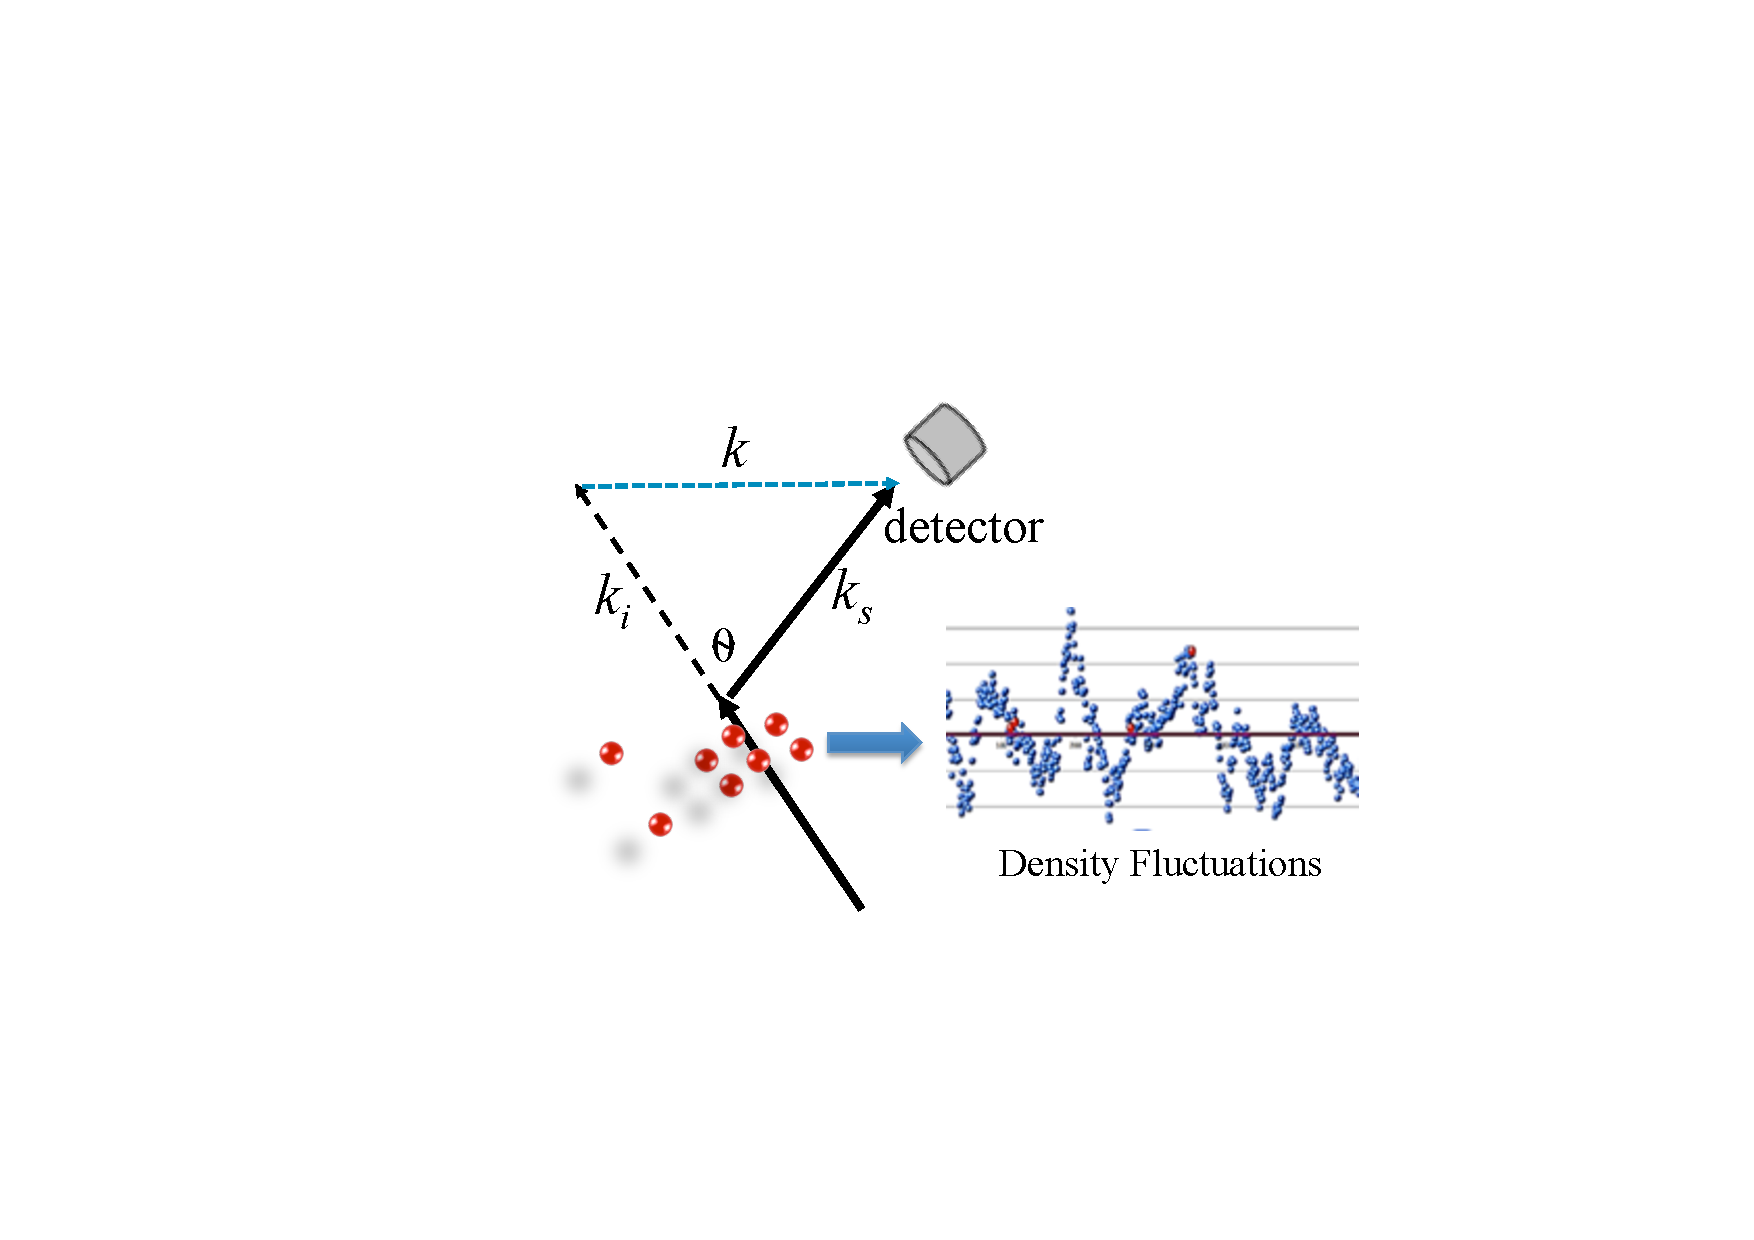
\includegraphics[width=0.4\textwidth]{Fig/SRBS_demo}
	\caption{ 自发瑞利-布里渊散射示意图\cite{Wu2020JFM},在气体中传播的光被气体分子自发的密度涨落散射.\\
		Schematic of the spontaneous Rayleigh-Brillouin scattering\cite{Wu2020JFM}, where the light is scattered by the spontaneous density fluctuations in the gas. 
	}
	\label{fig:RBS}
\end{figure}


\begin{figure*}[t]
	\centering
	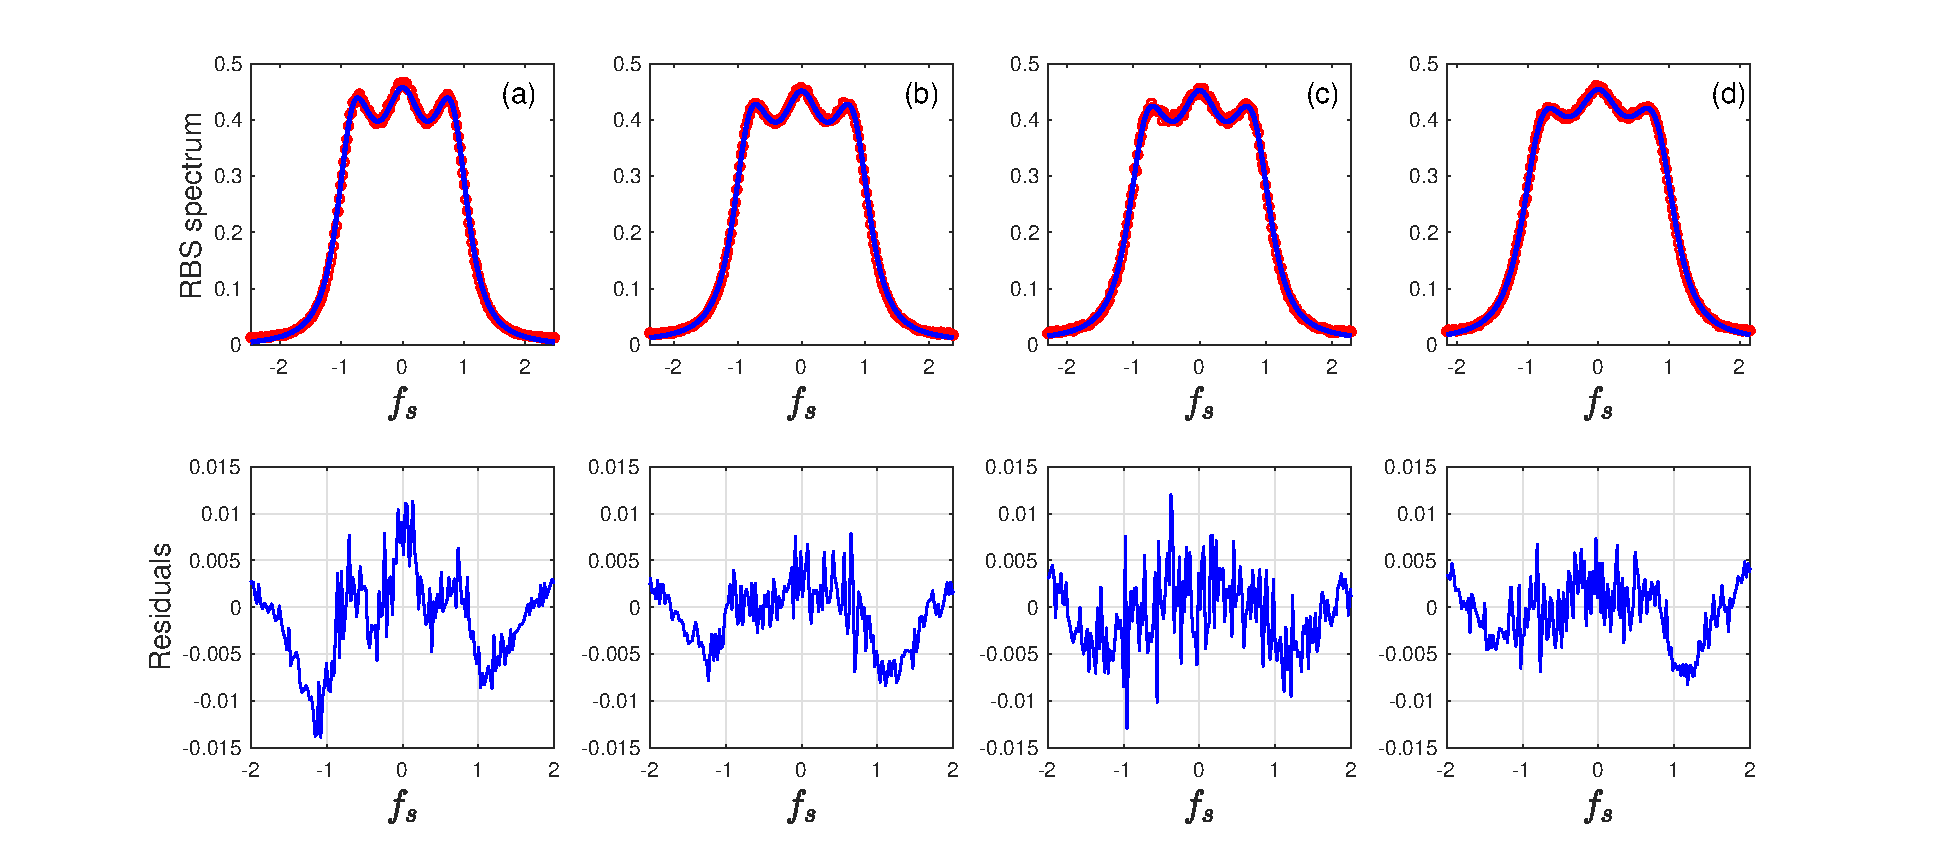
\includegraphics[scale=0.6,viewport=70 10 850 405,clip=true]{Fig/JFM10_Figure8.pdf}
	\caption{ 基于实验频谱 (圆圈) 和吴模型预测结果 (线条), 提取氮气的体积粘性与平动Eucken因子\cite{Wu2020JFM}. 第一行的实线为计算光谱,通过计算给定 $f_{tr}$ 和 $Z$ 范围内的最小误差. 第二行给出了实验光谱与理论光谱之间的误差. 实验与计算中所用到的参数汇总在表~\ref{table:N2}中. 频率 $f_s$ 由$v_m/\ell$归一化.\\
		Extraction of the bulk viscosity and translational Eucken factor of Nitrogen from the experimental spectra (circles) \cite{Wu2020JFM}. Lines in the first row show the spectra obtained from the Wu model, while those in the second row show the corresponding residuals between the experimental and theoretical spectra. Experimental conditions and extracted parameters are summarized in Table~\ref{table:N2}. The frequency $f_s$ is normalized by $v_m/\ell$.
	}
	\label{fig:N2}
\end{figure*}

\subsection{瑞利-布里渊散射}\label{RBS_section}

瑞利-布里渊散射指的是光在气体中传播时,被气体分子的自发密度涨落散射. 由于散射光谱包含气体信息,因此可以用来无损测量声速、流速、温度和体积粘性~\cite{Pan2002,Vieitez2010,guziyu}. 例如,欧洲航天局于2018年发射的ADM-Aeolus卫星,测量从地球表面到30公里高度的全球风速,用于提高天气预报精度. 

如图~\ref{fig:RBS}所示,波矢为 $\bm{k}_i$ 的入射光被散射,散射角为$\theta$,则散射波数为
$k=|\bm{k}_i-\bm{k}_s|=2|\bm{k}_i|\sin\left({\theta}/{2}\right)$.
散射光强度与光谱密度函数 $S(f_s)$相关,即密度扰动相关函数  $G(\bm{r},t)$ 的时空傅里叶变换. 假设散射波沿 $x_2$ 方向传播,相关函数和谱密度函数的解~\cite{Sugawara1968PoF,Reichl2016}为
\begin{align}
G(x_2,t) = \int_{-\infty}^{\infty}{n}(l+x_2,t){n}(l,0)dl,
\label{correlation function}
\end{align}
因此,频谱为
\begin{equation}\label{spectral density}
\begin{aligned}[b]
S(f_s) =& \int_{-\infty}^{\infty}\int_{-\infty}^{\infty}G(x_2,t)e^{i(kx_2-2\pi{f_s}t)}dx_2dt, 
\\
=& %\Re\left[2\int_{0}^{\infty}\int_{-\infty}^{\infty}G(x_2,t)e^{i(kx_2-2\pi{f_s}t)}dx_2dt\right].
\end{aligned}
\end{equation}
式中,$i$为虚数单位,${n}(x_2,t)$ 为密度扰动,$f_s$ 为散射频率.



对于短波长和高散射频率,应该使用气体动理论来描述密度扰动的演化过程. 以单原子气体为例说明瑞利-布里渊散射的计算. 密度扰动量与公式\eqref{chapter_vdf_lin_origin}中分布函数扰动量  $\phi$ 有关,初始密度脉动可定义为~\cite{Sugawara1968PoF,LeiJFM2015}:
$\phi(t=0,{x_2},\bm{\xi})\propto{}\delta({x_2})$. 取特征长度为散射波长$\ell=2\pi/k$,
通过时间上的拉普拉斯变换与空间上的傅里叶变换求解线性化玻尔兹曼方程\eqref{Chapter1_Boltzmann_lin0},可得
\begin{equation}\label{SRBS_LBE}
2\pi{i}(f_s-v_2)\hat{\phi}=\frac{\ell}{v_m}J(\hat{\phi})+1,
\end{equation}
其中方程右端的1来自于初始密度扰动对应的拉普拉斯变换,$\hat{\phi}(\bm{v})$ 分别对应 $\phi$ 的时空坐标下的拉普拉斯和傅里叶变换\cite{Gu2020AIA}. 散射频谱可通过以下公式计算
\begin{equation}\label{SRBS}
S(f_s)=\Re\left(\int \hat{\phi} f_{eq}(\bm{\xi})d\bm{\xi}\right),
\end{equation}
其中 $\Re$表示复数的实部.


\subsection{氮气分子的体积粘性与Eucken因子}
	\subsection{Bulk viscosity and Eucken factor of $\operatorname{N_2}$}

此例中,我们根据荷兰自由大学的实验数据\cite{guziyu}来提取氮气的体积粘性和平动Eucken因子. 其中,激光波长为 $ 366.8 $ 纳米,散射角为 $90^\circ$,因此等效波长为 $\ell=259.4$ 纳米. 实验条件下氮气的转动自由度与振动自由度分别为 $d_r=2$和0. 剪切粘性和热导率根据Sutherland公式计算. 通过调整吴模型中非弹性碰撞数和平动热导率,使得实验数据和数值模拟得到的频谱偏差最小. 表~\ref{table:N2}罗列了不同温度下气体物性参数和提取的碰撞数与热导率分量. %在吴模型中~\eqref{SRBS},通过修改平动与转动Eucken因子来恢复正确的热导率.


从上面的结果我们可以看出,误差函数存在全局最小值,并且为凸函数,因此,为了准确有效的确定转动碰撞数 $Z$ 和平动Eucken因子 $f_{tr}$,我们使用了以下方法.

	From the above results we find that the error function $E(Z,f_{tr})$ has one global minimum and is convex. Therefore, to accurately and efficiently determine $Z$ and $f_{tr}$, we adopt the following procedure. 

\begin{enumerate}
	\item 首先给定平动Eucken因子 $f_{tr}$,改变 $Z$的值, 并基于吴模型计算RBS频谱.然后将获得的光谱与响应函数卷积得到 $S_{WU}(f_s)$ 频谱,误差定义为:
	\begin{equation}\label{fitting_error}
	E(Z)=\sum_{\ell=1}^N\frac{\{S_{exp}[f_s(\ell)]-S_{WU}[f_s(\ell)]\}^2}{N},
	\end{equation} 
	式中,$N$ 是在实验中测量的离散频率数.将 $E$ 拟合为 $Z$ 的四次多项式,并找到该函数的最小值,进而可以找到最小误差将 $E_m(f_{tr})$ .此过程中,通常会计算6个不同的 $Z$ 值.
	%	where $N$ is the number of discrete frequencies measured in experiments. The minimum error $E_m(f_{tr})$ is found by fittingas the quartic polynomial function ofand finding the minimum of this quartic function. Typically 6 different values of $Z$ are calculated.
	
	\item 对于不同的 $f_{tr}$,重复步骤 1.与步骤1相同,通常会计算6个不同的 $f_{tr}$值.
	
	\item 将 $E_m(f_{tr})$ 拟合为 $f_{tr}$ 的四次多项式函数,进而确定函数最小值对应的 $f_{tr}$ .
	
	\item 使用步骤3得到的 $f_{tr}$,再次执行步骤1,以确定转动碰撞数 $Z$,最后可通过公式~\eqref{bulk_viscosity}确定体积粘性.
\end{enumerate}




\begin{table}
	\centering
	\caption{自发瑞利-布里渊散射实验中,氮气相关参数汇总以及根据吴模型从实验数据中提取的体积粘性与平动/转动Eucken因子. 剪切粘性与总热导率均使用国际单位制. \\
		Experimental conditions in the spontaneous Rayleigh-Brillouin scattering, and the extracted bulk viscosity, translational/rotational Eucken factors from the Wu model. The SI units are adopted for the shear viscosity and thermal conductivity.} %平动/内能Eucken因子均通过公式计算,其中,${\rho{D'}}/{\mu_s}=1.32$~\cite{mason1962heat},$f''_{tr}$ 与 $f''_{int}$ 也通过公式~\eqref{Eucken}计算而来,转动碰撞数~\cite{Parker1959}为实验测量值.
	\label{table:N2}
	\begin{tabular}{cccccccccc}
		\hline\hline
		& 实验 & $T$ (K)
		&  $10^5\mu_s $
		&  $100\kappa $  &  $P$ (bar)  & $\omega$ & $\mu_b/\mu_s$ & $f_{tr}$ & $f_{rot}$  \\
		& (a) &254.7 & $1.57$  & $2.28$ & 2.563  &0.80 &0.48   &2.16 &1.65 \\
		& (b) &275.2 & $1.67$  & $2.44$ & 2.784  &0.78 &0.61   &2.25 &1.53 \\
		& (c) &296.7 & $1.77$  & $2.60$ & 3.000  &0.76 &0.69   &2.31 &1.47\\
		& (d) & 336.6 & $1.95$ & $2.88$ & 3.400  &0.74 &0.94  &2.43 &1.33\\
		\hline\hline
				\hline	
				& 实验	& $f_{tr}$ & $f_{rot}$ & $f'_{tr}$ & $f'_{int}$  & $f''_{tr}$ & $f''_{int}$ \\
				& (a) &2.16 &1.65 &2.17 &1.58 & 2.12 & 1.61  \\
				& (b) &2.25 &1.53  &2.24 & 1.52 &2.14 &1.59 \\
				& (c) &2.31 &1.47  &2.27 &1.50 &2.16 &1.58 \\
				& (d) &2.43 &1.33 &2.33 &1.45 &2.18 &1.56	
			\\	\hline\hline
	\end{tabular}
\end{table}


实验结果与解析解的误差在1\%内,

实验数据与吴模型最佳预测的比较如图~\ref{fig:N2}所示. 实验~\cite{Lambert1977} 测得氮气在标准温度和压力下的转动弛豫时间为$\tau_r=7.4\times10^{-10}$ s,在$296.7$~K下,测得的氮气体积粘性为 $\mu_b=1.22\times10^{-5}\operatorname{kg\cdot{m^{-1}}\cdot{s^{-1}}}$. 根据公式~\eqref{bulk_viscosity}计算得到氮气的体积黏性为
\begin{equation*}
\mu_b=2p\tau_r\frac{d_r}{(3+d_r)^2}
=1.18\times10^{-5}\operatorname{kg\cdot{m^{-1}}\cdot{s^{-1}}}.
\end{equation*}
这一结果与实验值吻合较好. 另外, 提取的平动Eucken因子也在合理的范围.

Mason推导了WCU方程的Eucken因子解析解,而通过RBS试验同样可以得到平动Eucken因子与转动Eucken因子.本节将对这两组结果进行比较.在Mason的文章~\cite{mason1962heat}中,对于表~\ref{table:N2}中的温度,给定氮气的${\rho{D'}}/{\mu}=1.32$.将实验提取的转动碰撞数  $Z$ 代入Eucken因子解析解中,并与表~\ref{table:N2}的实验数据进行比较.对比结果表明:$f_{tr}$ 与 $f'_{tr}$,以及$f_{rot}$ 与 $f'_{int}$较为一致,最大相对偏差不大于10\%.进一步地,考察了平动Eucken因子与转动Eucken因子解析解与测量值的区别.对于单原子气体,玻尔兹曼方程的输运系数解析解与实验值吻合较好,相对误差小于 $  2\% $,对于分子气体,输运系数的解析解与实验数据差别较大,这可能是因为在解析解的推导过程中引入了近似值.

 从建模的角度出发,经典模型方程把分子气体运动中的弹性碰撞与非弹性碰撞看做是简单的弛豫过程. 

\section{总结与展望}

本文回顾了国内外学者在稀薄效应动理学建模中所取得的进展,包含单原子气体与分子气体. 由于高温真实气体效应,当分子内自由度增加时,分子间复杂的相互作用通常伴随着更加新颖、复杂的物理现象,这对稀薄分子气体动理学建模提出了很高的要求. 我们指出应力偏量、能量交换、热流的弛豫过程是输运现象的本质,而剪切粘性、体积粘性、平动/内部热导率等输运系数则是表象,即,随着克努森数的变化,这些输运系数对应的本构关系会失效,而相应的弛豫过程和速率不会改变. 为了准确预测稀薄分子气体的非平衡行为,气体动理学的建模过程应尽可能准确地捕捉应力偏量、能量交换、热流的弛豫过程和速率. 


本文还介绍了DSMC中提取热弛豫速率 的方法,并讨论了DSMC方法恢复热导率的能力. 虽然经典的Larsen-Borgnakke模型可以通过调整非弹性碰撞概率改变体积粘性,但是很难同时调整热导率及其分量. 而这些分量的比例以及本质的热流弛豫时间对稀薄气体流动的影响巨大. 因此,非常有必要对DSMC碰撞模型进行修改和优化.

非常有意思的是,基于王承书等人的工作,分子气体的线性化理论和方法已经非常成熟. 而非线性模型虽然五花八门,但都与线性化模型存在着本质联系,即所有的非线性模型都可以通过对线性化Gross-Jackson模型和Hanson-Morse模型的非线性化而来. 本文首次给出一个非线性化方案.  
%
%对于临近空间高超声速飞行器而言,其周围的空气动力学非常复杂. 如何建立描述多组分气体、化学反应的稀薄气体动理学模型是个极大的挑战. 本文提出的弛豫过程本质论、输运系数表象论、从线性化模型中反推非线性模型的方法,以及从分子动力学和相关实验中提取弛豫速率的设想,将为解决此类问题提供极大助力.

